\documentclass[twoside]{report}

\usepackage{preamble}

\begin{document}

% Título
\begin{titlepage}
    \begin{center}
    
    \vspace*{1cm}
    
    \Huge
    \textbf{\Lenguaje{}}
    
    \vspace{0.5cm}
    
    \Large
    Implementación de un lenguaje Pascal-Like
    
    \vspace{1.5cm}
    
    \textbf{Matías Federico Gobbi}
    
    \vfill
    
    
\includegraphics[width=0.5\textwidth]{UNC.png}
    
    Facultad de Matemática, Astronomía y Física
    \\
    Universidad Nacional de Córdoba
    \\
    \today
            
    \end{center}
\end{titlepage}

\chapter*{Resumen}
% Resumen
Este trabajo consiste en el diseño e implementación de un lenguaje de programación estructurado basado en el lenguaje \Pascal{}, orientado al aprendizaje de algoritmos y estructura de datos.
El mismo es utilizado actualmente en una materia de la facultad, contando con una definición informal.
Existe una sintaxis concreta relativamente consolidada aunque no especificada, y la semántica está definida de manera intuitiva.
En el trabajo se estudió la información disponible a partir del dictado de la materia obteniendo una definición formal de la sintaxis abstracta, en conjunto con la definición de varios chequeos estáticos, como el sistema de tipos.
% Finalmente definimos una semántica \textit{small step} a partir de la cual implementamos un intérprete interactivo en el lenguaje \Haskell{}.
% Describir Estructura de Tesis: Detallar Formato de Capítulos!

\tableofcontents

\chapter{Introducción}
% Introducción
En el siguiente trabajo, desarrollaremos un lenguaje de programación para la materia \Materia{}.
Antes de comenzar propiamente con la definición formal e implementación del mismo, lo correcto es presentar los objetivos que nos hemos impuesto para la creación del lenguaje, y las motivaciones que nos han impulsado al desarrollo de este proyecto.
Por lo tanto, la siguiente sección introducirá al lector los distintos aspectos que influyeron la formación del lenguaje, y justificaron la realización de este trabajo.

\section{Motivación}

En la materia \Materia{}, durante varios años, se ha utilizado un pseudocódigo para la enseñanza de los distintos conceptos que se estudian en la misma.
Debido a esto, el lenguaje que diseñamos (basado en este pseudocódigo) tendrá un fin didáctico, y busca ser otra fuente de aprendizaje para auxiliar el dictado de la asignatura.
Los ejes principales de la materia consisten en el análisis de algoritmos, la definición de tipos abstractos de datos, y la comprensión de diversas técnicas de programación.

El objetivo del pseudocódigo es poder introducir a los estudiantes a nuevos conceptos y fomentar buenas prácticas de programación.
Se utiliza para describir de forma precisa principios operacionales de los distintos algoritmos estudiados en la materia.
Típicamente, se omiten detalles esenciales para la implementación de los algoritmos para favorecer el entendimiento de los mismos.
No existe ningún estándar para la sintaxis o semántica del pseudocódigo, por lo que un programa en este pseudo-lenguaje  no es ejecutable en el sentido que no puede ser traducido a una serie de instrucciones máquina.

Nuestra meta final con este proyecto, es poder tomar la totalidad de los fragmentos de pseudocódigo que se encuentran dispersos en los diversos contenidos de la materia, y transformarlos en un lenguaje completamente implementado, con todo lo que esto implica.
Obviamente, nuestro principal desafío para cumplir nuestra tarea, es poder resolver las distintas ambigüedades y la falta de especificación que el actual pseudocódigo presenta.

\subsection{Objetivos de la Asignatura}

Durante el desarrollo de la materia, se pretende que el alumno adquiera diversos conceptos relacionados con los distintos temas estudiados en la asignatura.
Algunos de los mismos son listados a continuación:
\begin{itemize}
    \item Capacidad para comprender y describir el problema que resuelve un algoritmo (el \textit{qué}), y diferenciarlo de la manera en que lo resuelve (el \textit{cómo}).
    \item Suficiencia para analizar algoritmos, compararlos según su eficiencia en tiempo de ejecución y en espacio de almacenamiento.
    \item Hábito de identificar abstracciones relevantes al abordar un problema computacional, y aptitud para la especificación e implementación de las mismas.
    \item Familiaridad con técnicas de diseño de algoritmos de uso frecuente, y comprensión de diversos algoritmos conocidos.
    \item Contacto con la programación (principalmente en el lenguaje \C{}) de algoritmos y estructura de datos.
    \item Aptitud para la utilización de diversos niveles de abstracción y adaptación a distintos lenguajes de programación.
\end{itemize}

\subsection{Programa de la Asignatura}

El contenido de la materia se puede dividir en tres unidades.
En cada una de estas, se introducen nuevos conceptos que luego se reflejan en diversos fragmentos de pseudocódigo empleados para facilitar la comprensión de los mismos.
En el diseño del futuro lenguaje, se deberán tener en cuenta todas estas cuestiones para poder crear una herramienta útil para complementar la enseñanza de la asignatura.

\subsubsection{Análisis de Algoritmos}

La primer unidad de la materia, se basa en el análisis de algoritmos.
Inicialmente, se estudian distintas maneras de ordenar arreglos utilizando diversas técnicas, como \textit{ordenación por selección}, \textit{ordenación por inserción}, \textit{ordenación por intercalación}, \textit{ordenación rápida}, entra otras.
Con estos contenidos básicos presentes, se enseña al alumno a contar operaciones de un programa, introduciendo de esta forma los conceptos de \textit{orden} y \textit{jerarquía} sobre la complejidad de un algoritmo.
Para terminar, se introducen las recurrencias \textit{divide y vencerás}, y se presentan otros algoritmos como la \textit{búsqueda lineal}, y la \textit{búsqueda binaria}.

\subsubsection{Estructura de Datos}

La segunda parte de la materia, presenta la noción de estructuras de datos.
Se describen a los \textit{tipos concretos} como un concepto relativo a un lenguaje de programación, donde se estudian elementos como los arreglos, las listas, los registros, y los tipos enumerados.
Mientras, los \textit{tipos abstractos} se presentan como una idea asociada a un problema que se quiere resolver.
Se describe la diferencia entre la \textit{especificación}, y la \textit{implementación} de los mismos, y se enseña la importancia de la elección adecuada para estos.
Se examinan diseños distintos para varios de los diversos \textit{TAD's}, como el \textit{contador}, la \textit{pila}, la \textit{cola}, y el \textit{árbol}, junto con la eficiencia en tiempo o espacio de sus distintas operaciones.
Además, se introduce el concepto de \textit{manejo dinámico de memoria} de un programa mediante el uso de punteros.

\subsubsection{Algoritmos Avanzados}

La última unidad, presenta distintas estrategias conocidas para la resolución de problemas algorítmicos.
Se introduce el esquema general de los \textit{algoritmos voraces}, y se enseñan diversos algoritmos que se basan en esta idea como el de \textit{Dijkstra}, \textit{Prim}, y \textit{Kruskal}.
También se introduce al concepto de \textit{backtracking}, resolviendo los problemas de la \textit{moneda}, y la \textit{mochila}, entre otros.
Luego, se ve \textit{programación dinámica} donde se visitan problemas previos, además de ver nuevos conceptos como el algoritmo de \textit{Floyd}.
Un último tema que se enseña en la materia, es la recorrida de grafos, y las distintas variantes para realizar la misma.

\section{Características del Lenguaje}

Una vez detallados los fundamentos en los que se basa el lenguaje, es hora de describir sus características más importantes.
\Lenguaje{} es una formalización del pseudocódigo utilizado en la materia \Materia{}, por lo que está diseñado para enseñar conceptos fundamentales de forma clara y natural.
Es un lenguaje imperativo similar a \Pascal{}.
Este último fue diseñado por \textit{Niklaus Wirth} cerca de 1970 \cite{Pascal}.
Algunos elementos básicos que comparten son:
\begin{itemize}
    \item Una sintaxis verbosa, pero fácil de leer.
    \item Un tipado fuerte para las expresiones.
    \item Un formato estructurado del código.
\end{itemize}

Al solo contar con una definición informal e incompleta del pseudocódigo, tuvimos que enfrentarnos a problemas de ambigüedad y falta de especificación para la creación del lenguaje.
Debido a esto, la transición de uno a otro puede no ser inmediata.
De todas formas, la esencia de ambos es la misma.
La sintaxis del lenguaje es rigurosa, en comparación al código de la materia que era flexible en este aspecto.
La semántica del primero está definida de forma precisa, a diferencia del pseudocódigo que solo se contaba con la intuición del lector para interpretar la misma.

\subsection{Tipado}

Como mencionamos previamente, \Lenguaje{} posee tipado fuerte.
Esto significa que no se permiten violaciones de los tipos de datos, es decir, dado el valor de una variable de un tipo determinado, no se puede usar la misma como si fuera de otro tipo distinto al especificado en el programa.
En una primera instancia, no hay ninguna especie de conversión, implícita o explícita, para los tipos de las expresiones del lenguaje.

En \Lenguaje{} se ofrecen una serie de tipos nativos un poco más limitada a la utilizada en el pseudocódigo de la materia.
Los mismos, a su vez, se pueden dividir en tipos básicos y en tipos estructurados.
Al mismo tiempo, existe la posibilidad de definir nuevos tipos de datos en el lenguaje; aspecto fundamental para el desarrollo de la segunda unidad de la asignatura.

Los tipos nativos básicos del lenguaje son los enteros, los reales, los booleanos y los caracteres.
Para manipular valores de estos tipos, se ofrecen las operaciones aritméticas y lógicas típicas.
A su vez, también se encuentran definidas las operaciones de igualdad y orden para estos valores, a pesar que su aplicación no se limita solo a los mismos.

Por otro lado, los tipos estructurados incorporados son los arreglos y los punteros.
Los primeros tendrán un funcionamiento similar a los especificados en el lenguaje \C{}.
Además, existirá la posibilidad de definir arreglos multidimensionales, y arreglos cuyos tamaños serán variables.
Los segundos, permitirán el manejo dinámico de la memoria de un programa y serán útiles para la creación de nuevos tipos de datos.

Finalmente, el usuario podrá crear sus propios tipos de datos.
Hay tres posibilidades para la declaración de estos.
Los tipos enumerados representarán una enumeración de un conjunto finito de valores.
Los sinónimos serán un renombrado de un tipo ya existente.
Y las tuplas permitirán la creación de estructuras con múltiples campos.
Todos estos elementos serán fundamentales para el estudio de los \textit{TAD's} en la materia.

Similar a \Haskell{}, en el lenguaje existen ciertas clases predefinidas que caracterizan el comportamiento de los tipos que las implementan.
Estas son \textbf{Eq}, \textbf{Ord}, e \textbf{Iter}.
La primera, será implementada por todos los tipos que se pueden igualar.
La segunda, es satisfecha por las categorías de elementos que son ordenables.
Finalmente, la última clase indica si cierta estructura puede ser recorrida de forma iterativa.
Una vez que el usuario declara un tipo, puede implementar todas las operaciones que una determinada clase requiera, para convertir a su nueva estructura de datos en una instancia de la misma.

\subsection{Polimorfismo}

El lenguaje permite la declaración de funciones y procedimientos con polimorfismo paramétrico.
Esto significa que con una única definición, independiente de los tipos específicos de las entradas polimórficas, las funciones y procedimientos tendrán la capacidad de ser aplicables a argumentos con valores de distinto tipo.
A su vez, esto introduce la capacidad de trabajar con variables de tipo en el programa, cuyos tipos concretos serán resueltos en tiempo de ejecución.

Otra posibilidad que permite el lenguaje, es agregar restricciones de clases que deberán ser satisfechas por las variables de tipo que los procedimientos y funciones introducen en su prototipo.
Con este refinamiento, uno puede abstraerse de los tipos específicos en la implementación, para solo considerar las operaciones básicas que los mismos proporcionan.
De esta forma, podemos limitarnos a trabajar con valores que ofrecen ciertas propiedades como la de igualdad, la de orden, y la de ser iterables.

El polimorfismo que admiten las funciones y procedimientos del lenguaje no se limita solo a tipos.
También existe una especie de polimorfismo para los tamaños de arreglos que se introducen en la declaración de los anteriores.
Con esta posibilidad, se pueden definir funciones o procedimientos que operan sobre arreglos, independientemente del tamaño de estos.
Esto introduce la capacidad de trabajar con tamaños variables de arreglos, cuyo tamaño concreto será resuelto durante la ejecución del programa.

\subsection{Recursión}

La recursión es otro de los temas fundamentales en el dictado de la materia.
En particular, para la parte de conteo de operaciones, donde se estudia como calcular el \textit{orden} de un algoritmo.
Dentro del cuerpo de una función o procedimiento, se puede realizar una llamada recursiva a si mismo para continuar con la ejecución del programa.
En estas situaciones, el lenguaje no presenta ninguna particularidad relevante como para ser mencionada en esta sección.

En cambio, donde si haremos una salvedad, es en la declaración de tipos de datos.
En el lenguaje, solo se permite una clase de recursión muy limitada para los mismos.
Para crear un tipo recursivo, solo hay una posibilidad bastante restrictiva, y es en la definición de una tupla que posea un campo de tipo puntero.
Esta especie de recursión es lo suficientemente expresiva como para permitir la implementación de listas enlazadas en el lenguaje, concepto fundamental en el programa de la asignatura.

\subsection{Manejo de Memoria}

Una característica muy importante del pseudocódigo, que se sigue manteniendo en el lenguaje, es el manejo dinámico de memoria.
Durante la segunda y tercera parte de la materia, este es un concepto central que acompaña al desarrollo de la asignatura.
Para la implementación de \textit{TAD's}, resulta un tema recurrente que sirve para comparar distintos diseños en base a su claridad, portabilidad, y eficiencia.

Mediante el uso de punteros, y la llamada de los procedimientos especiales \textbf{alloc} y \textbf{free}, el usuario puede hacer un uso explícito sobre la memoria utilizada por el programa.
Con algunos conceptos similares a \C{}, uno puede reservar memoria que será accesible mediante el uso de punteros.
Durante la ejecución del programa, se podrá manipular la memoria reservada y, cuando ya no sea necesaria, se podrá liberar la misma.

\subsection{Encapsulamiento}

Una última característica relevante que fue tomada de los contenidos de la materia y sentó las bases para el desarrollo del lenguaje, es el encapsulamiento.
En el pseudocódigo esta particularidad muchas veces era omitida, debido que un programa en este pseudo-lenguaje solo se podía ejecutar \textit{en el aire}.
Debido a esto, se contaba con una intuición sobre que era parte de la especificación y que era parte de la implementación de un tipo de dato, de manera informal.

Cuando pasamos al lenguaje formal, hay una evidente diferenciación entre el código que se utiliza para especificar un \textit{TAD}, y el código empleado para su implementación.
En \Lenguaje{} se busca tener una clara separación en módulos para los elementos definidos de un programa.
De esta forma, podemos abstraernos de los detalles propios de la implementación de una estructura de datos, y basarnos solo en su especificación para resolver cierto problema algorítmico.

\section{Desarrollo del Intérprete}

Debido que el objetivo de este proyecto es la creación de un lenguaje de programación, nuestro ideal es que el producto final del trabajo sea la implementación de un intérprete para el mismo.
El desarrollo de esta herramienta no es una actividad trivial, por el contrario, su avance requerirá de múltiples iteraciones y se dividirá en distintas etapas donde, a medida que se progrese en el proyecto, habrá una retroalimentación mutua entre las mismas.
Con respecto a este trabajo de tesis en particular, realizaremos la implementación para la primera versión de la fase de \textit{análisis} del intérprete.
En la misma, luego de definir la sintaxis del lenguaje, desarrollaremos tanto el parser como los chequeos estáticos que conforman esta etapa.

A continuación, daremos un breve marco teórico sobre distintas cuestiones que consideramos importante mencionar sobre el diseño del intérprete en general.
Para el mismo, nos basaremos en los primeros capítulos de la bibliografía de Aho, Sethi y Ullman \cite{Dragon}.

\begin{figure}[h]
\centering
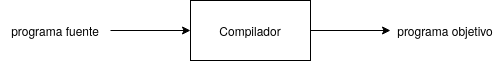
\includegraphics[scale=0.5]{Compilador.png}
\caption{Un compilador}
\label{Compilador}
\end{figure}

Un lenguaje de programación es una notación para describir computaciones a personas y a máquinas.
Pero para que un programa sea ejecutable, antes debe ser traducido a un formato comprensible para una máquina.
Los sistemas de software que se encargan de esta traducción son denominados \textit{compiladores}.
De forma simple, un compilador es un programa que puede leer un programa especificado en un \textit{lenguaje fuente} y traducirlo en un programa equivalente en un \textit{lenguaje objetivo}.
En la imagen \ref{Compilador} se puede observar un esquema simplificado de esta idea.

Un intérprete es otra clase común de procesador de lenguajes.
En lugar de producir un programa objetivo como resultado de una traducción, un intérprete simula ejecutar directamente las operaciones especificadas en el programa fuente, en base a las entradas suministradas por el usuario y retornando las salidas producidas como resultado de la ejecución.
En la figura \ref{Intérprete} se puede apreciar la diferencia esencial entre ambas clases de procesadores de lenguajes.

\begin{figure}[h]
\centering
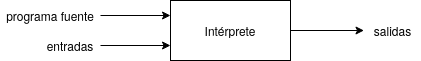
\includegraphics[scale=0.5]{Interprete.png}
\caption{Un intérprete}
\label{Intérprete}
\end{figure}

Si entramos un poco más en detalle, podemos observar que el proceso de transformación está compuesto por dos etapas: \textit{análisis} y \textit{síntesis}.
En el caso de la primera etapa, su desarrollo puede realizarse de manera idéntica tanto para compiladores como para intérpretes.
En cambio, la segunda presenta diferencias sustanciales entre ambos.
Debido que nuestro objetivo es implementar un intérprete para el lenguaje, nos concentraremos solo en el estudio de este.

\subsection{Análisis}

La parte del análisis divide el programa fuente en distintas piezas e impone una estructura gramatical a las mismas.
Luego, utiliza esta estructura para crear una representación intermedia del programa fuente.
Si la etapa de análisis detecta que el programa presenta errores sintácticos o incoherencias semánticas, entonces deberá proveer mensajes informativos para que el usuario pueda aplicar las correcciones adecuadas.
En nuestro caso, la representación intermedia que utilizaremos serán los \textit{arboles de sintaxis abstracta}.
La transformación del programa fuente a nuestra representación intermedia, no es trivial.
Para facilitar la misma, comúnmente se divide esta tarea en varias fases.

\subsubsection{Análisis Léxico}

En esta etapa, también llamada \textit{fase de escaneo}, se analiza la entrada carácter por carácter y se divide la misma en una serie de unidades elementales denominadas \textit{componentes léxicos}.
Por cada componente léxico, la fase de escaneo produce como salida un \textit{token} que pertenece a cierta categoría gramatical y posee una cantidad determinada de atributos con información relevante para las siguientes fases de análisis.
En esta etapa, además, se filtran elementos como los espacios en blanco y los comentarios.

\subsubsection{Análisis Sintáctico}

Esta es la fase que comúnmente se denomina \textit{parser}.
El parser utiliza los tokens obtenidos en la etapa previa, para crear una representación intermedia de la estructura gramatical del flujo total de tokens.
Como mencionamos anteriormente, nosotros utilizaremos un \textit{árbol de sintaxis abstracta} como representación.
Las fases posteriores del intérprete emplearán esta estructura gramatical para continuar el análisis del programa fuente.

\subsubsection{Análisis Semántico}

La última etapa del análisis es la de \textit{chequeos estáticos}.
La misma se encarga de verificar si las restricciones semánticas impuestas en la definición del lenguaje son respetadas.
Una parte importante de este análisis es el llamado chequeo de tipos (\textit{typecheck}).
Comúnmente, esta fase toma como entrada la representación intermedia obtenida en la etapa previa, y le agrega las anotaciones de tipos adecuadas, necesarias para continuar el análisis en etapas posteriores.

\subsection{Síntesis}

La parte de síntesis de un compilador es muy diferente a la de un intérprete.
Para el primero, tenemos que construir el programa objetivo utilizando la representación intermedia, junto con toda la información adicional recopilada en las etapas previas.
Habitualmente, esta fase se divide en otras dos partes, la \textit{generación de código intermedio} y la \textit{generación de código objeto}.
En la \textit{generación de código intermedio} se obtiene una representación independiente de la máquina, pero fácilmente traducible a lenguaje ensamblador.
En cambio, la \textit{generación de código objeto} es totalmente dependiente de la arquitectura concreta para la que se esté desarrollando el compilador.
Además, durante estas fases comúnmente se aplica algún proceso de optimización sobre el código generado.

Del otro lado, como el objetivo de un intérprete difiere con el de un compilador, sus etapas de síntesis también lo hacen en la misma manera.
Para obtener los resultados del programa, debemos partir del \textit{árbol de sintaxis abstracta} obtenido luego de la fase de \textit{análisis} del intérprete y, junto con los datos de entrada sustentados por el usuario, simular la ejecución del programa en base a las acciones especificadas en el código del mismo.
De esta forma, una vez finalizada la ejecución, se obtienen las salidas del programa.
En la imagen \ref{Fases} se puede observar la estructura de nuestro intérprete.

\begin{figure}[h]
\centering
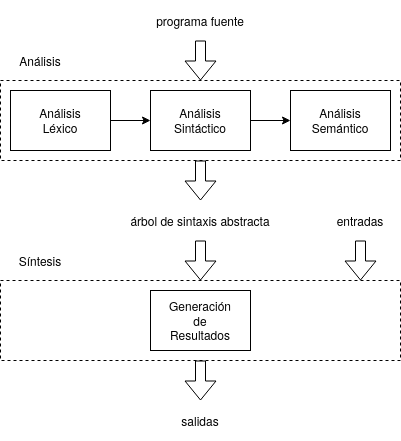
\includegraphics[scale=0.5]{Fases.png}
\caption{Estructura de un intérprete}
\label{Fases}
\end{figure}

% Ideas!!
\iffalse

% cosas que faltan
* Manejo de errores y excepciones
* canales de input y output

% concepto
Introducción: Presentar lo que estamos haciendo, es decir, contar que hay un lenguaje definido informal e incompletamente con el que se enseña una materia. Presentar ejemplos de todo lo que se hace con el lenguaje. Como si se lo contaras a alguien que sabe de programación pero no cursó la materia.
Contaríamos también qué cosas NO están bien definidas, qué ambigüedades encontramos, etc

% idea
la idea que tengo es que en la introducción hablamos de las características del lenguaje, y de lo que se enseña en la materia con él
pero no hablamos del lenguaje en particular
o sea, podemos dar algún ejemplo
pero no es que presentamos "el lenguaje tiene estas instrucciones: blablabl"
sino que decimos que es un lenguaje imperativo, que tiene manejo de memoria, etcétera
mencionamos todas las características
pero no damos formalmente nada
en el primer capítulo sí presentaríamos más detalladamente el lenguaje, como un tutorial
(el lenguaje nuestro, ya bien definido)
(pero no formalmente, sino como tutorial)
o sea, luego de leer la introducción, el lector tiene que saber de qué se trata el lenguaje, qué características tiene (o queremos que tenga), que cosas NO tiene
(y no va a tener)
pero no es que leyendo la intro lo vaya a aprender a usar
cuando lea el primer capítulo sí ya puede programar
a partir del capítulo 2 ya sería algo técnico
de cómo lo implementamos

% finalidad
incluida la finalidad con respecto a la materia también

% motivación
o sea, lo que yo dije es medio breve
me parece bueno que primero esté la motivación
¿por qué otro lenguaje?
o sea, no es que estamos definiendo un lenguaje imperativo porque tenemos ganas
sino que hay un motivo inicial
y es didáctico
así que sí, hay que hablar de la materia y de los conceptos que se enseñan con este lenguaje (que son muchísimos)

% estructura
o sea imagino de mínima:
Intro:
* Motivación
* Características del lenguaje
* Organización general de la tesis

% diferencias
pero no se pretende que alguien lea la intro y pueda programar
se pretende que alguien entienda por qué queremos implementar este lenguaje, y qué características tiene

% características
deberíamos hablar de tipado, de polimorfismo, de encapsulamiento
deberíamos hablar de manejo de memoria
de qué conceptos se enseñan en la materia
\fi

\chapter{Sobre el lenguaje}

\chapter{Sobre el parser}
% Sintaxis
En el siguiente capítulo, nos dedicaremos principalmente a la definición del lenguaje.
Se precisará de manera formal su sintaxis abstracta, y se presentará de manera informal su sintaxis concreta.
Una vez definidas, comenzaremos con la descripción de los aspectos principales sobre la implementación del parser de \Lenguaje{}.
%Idealmente, esta sección del trabajo formará parte de la documentación del futuro intérprete.

\section{Sintaxis Abstracta}

La sintaxis del lenguaje ya se expuso de manera informal en el capítulo anterior, mediante los distintos ejemplos que se fueron ilustrando a lo largo del desarrollo. A continuación, describiremos de manera formal la \textit{sintaxis abstracta} de \Lenguaje{}, como ya mencionamos esta sintaxis
pretende capturar las componentes relevantes de las distintas construcciones sintácticas del lenguaje eliminando detalles poco relevantes de una sintaxis
concreta.
%A pesar de esta situación, si se quisiera hacer un estudio formal del lenguaje, lo correcto sería dar una definición precisa de su sintaxis.
%Por lo tanto, a continuación se describirá la \textit{sintaxis abstracta} de \Lenguaje{}.

\subsection{Expresiones}

Una expresión puede adoptar distintas formas; puede ser un valor constante, una llamada a función, una operación sobre otras expresiones, o una variable con sus respectivos operadores.
Su composición se describe a continuación.

\begin{lstlisting}[style = syntax]
$\NT{expression}$ $::=$ $\NT{constant}$ | $\NT{functioncall}$ | $\NT{operation}$ | $\NT{variable}$
\end{lstlisting}

Una constante puede pertenecer a alguna de las siguientes clases de valores.
Los no terminales $\NT{integer}$, $\NT{real}$, $\NT{bool}$, y $\NT{character}$ denotan los conjuntos de valores esperados, mientras que $\NT{cname}$ hace referencia a los identificadores de constantes enumeradas definidas por el usuario.
Los terminales \textbf{inf} y \textbf{null}, representan al infinito y al puntero nulo respectivamente.

\begin{lstlisting}[style = syntax]
$\NT{constant}$ $::=$ $\NT{integer}$ | $\NT{real}$ | $\NT{bool}$ | $\NT{character}$ | $\NT{cname}$ | $\T{inf}$ | $\T{null}$
\end{lstlisting}

Una llamada a función está compuesta por su nombre, y la lista de argumentos que recibe; la cual puede tener una cantidad arbitraria de parámetros.
Notar que se utilizará la misma clase de identificadores tanto para funciones y procedimientos, como para variables.

\begin{lstlisting}[style = syntax]
$\NT{functioncall}$ $::=$ $\NT{id}$ $($ $\NT{expression}$ $\ldots$ $\NT{expression}$ $)$
\end{lstlisting}

Los operadores del lenguaje están conformados por las operaciones numéricas y booleanas tradicionales, y por los operadores de orden e igualdad respectivos a las clases definidas.
Observar que será necesario la implementación de un chequeo de tipos para asegurar su uso apropiado.

\begin{lstlisting}[style = syntax]
$\NT{operation}$ $::=$ $\NT{expression}$ $\NT{binary}$ $\NT{expression}$ | $\NT{unary}$ $\NT{expression}$

$\NT{binary}$ $::=$ $+$ | $-$ | $*$ | $/$ | $\%$ | $||$ | $\&\&$ | $<=$ | $>=$ | $<$ | $>$ | $==$ | $!=$

$\NT{unary}$ $::=$ $-$ | $!$
\end{lstlisting}

Finalizando con las expresiones, describiremos a las variables con sus respectivos operadores.
Una variable puede simbolizar un único valor, un arreglo de varias dimensiones, una tupla con múltiples campos, o un puntero a otra estructura en memoria.
El no terminal $\NT{fname}$ representa el nombre de un campo de una estructura de tipo tupla definida por el usuario.

\begin{lstlisting}[style = syntax]
$\NT{variable}$ $::=$ $\NT{id}$
         | $\NT{variable}$ $[$ $\NT{expression}$ $\ldots$ $\NT{expression}$ $]$
         | $\NT{variable}$ $.$ $\NT{fname}$
         | $\star$ $\NT{variable}$
\end{lstlisting}

\subsection{Sentencias}

Las sentencias del lenguaje se dividen en las siguientes construcciones.
La composición de la \textit{asignación} y el \textit{while} es bastante simple, por lo que se detallan también a continuación.
Notar que el no terminal $\NT{sentences}$ se utiliza para representar al bloque de sentencias.

\begin{lstlisting}[style = syntax]
$\NT{sentence}$ $::=$ $\T{skip}$ | $\NT{assignment}$ | $\NT{procedurecall}$ | $\NT{if}$ | $\NT{while}$ | $\NT{for}$

$\NT{assignment}$ $::=$ $\NT{variable}$ $:=$ $\NT{expression}$

$\NT{while}$ $::=$ $\T{while}$ $\NT{expression}$ $\T{do}$ $\NT{sentences}$

$\NT{sentences}$ $::=$ $\NT{sentence}$ $\ldots$ $\NT{sentence}$
\end{lstlisting}

Para la llamada de procedimientos, se utiliza una sintaxis idéntica a la empleada para la llamada de funciones.
Adicionalmente se encuentran definidos los procedimientos especiales \textbf{alloc} y \textbf{free}, exclusivos para el manejo dinámico de memoria del programa.

\begin{lstlisting}[style = syntax]
$\NT{procedurecall}$ $::=$ $\NT{id}$ $($ $\NT{expression}$ $\ldots$ $\NT{expression}$ $)$
             | $\T{alloc}$ $\NT{variable}$
             | $\T{free}$ $\NT{variable}$
\end{lstlisting}

La especificación de la sentencia \textit{if} es compleja en lo que refiere a su sintaxis concreta.
Para simplificar la sintaxis abstracta, nos limitaremos a solo permitir una única alternativa para su especificación.
%Notar que las versiones complejas de la sentencia, empleadas en capítulos anteriores, pueden ser definidas mediante azúcar sintáctico.

\begin{lstlisting}[style = syntax]
$\NT{if}$ $::=$ $\T{if}$ $\NT{expression}$ $\T{then}$ $\NT{sentences}$ $\T{else}$ $\NT{sentences}$
\end{lstlisting}

Finalizando con las sentencias, otra instrucción que presenta varias alternativas es el \textit{for}.
Con la sentencia es posible declarar una variable, la cual tomará valores en un rango determinado, y ejecutar de forma iterada un bloque de sentencias específico.
Los rangos ascendentes se definen con \textbf{to}, y los descendentes con \textbf{downto}.

\begin{lstlisting}[style = syntax]
$\NT{for}$ $::=$ $\T{for}$ $\NT{id}$ $:=$ $\NT{expression}$ $\T{to}$ $\NT{expression}$ $\T{do}$ $\NT{sentences}$
      | $\T{for}$ $\NT{id}$ $:=$ $\NT{expression}$ $\T{downto}$ $\NT{expression}$ $\T{do}$ $\NT{sentences}$
\end{lstlisting}

\subsection{Tipos}

Los tipos que soporta \Lenguaje{} pueden dividirse en dos categorías, los nativos del lenguaje y los definidos por el usuario.
A su vez los nativos puede separarse en básicos (\textbf{int}, \textbf{real}, \textbf{bool}, \textbf{char}), y estructurados ($\NT{array}$, $\NT{pointer}$).

\begin{lstlisting}[style = syntax]
$\NT{type}$ $::=$ $\T{int}$ | $\T{real}$ | $\T{bool}$ | $\T{char}$
      | $\NT{array}$
      | $\NT{pointer}$
      | $\NT{definedtype}$
      | $\NT{typevariable}$
\end{lstlisting}

Del lado de los tipos nativos estructurados, se tienen a los arreglos y a los punteros.
Para los primeros, hay que especificar como se definen los tamaños para sus dimensiones.
El no terminal $\NT{sname}$ representa a los identificadores de tamaño dinámico introducido en el prototipo de funciones y procedimientos.
Para los segundos, solo se debe indicar cual es el tipo de valores que se va a referenciar.

\begin{lstlisting}[style = syntax]
$\NT{array}$ $::=$ $\T{array}$ $\NT{arraysize}$ $\ldots$ $\NT{arraysize}$ $\T{of}$ $\NT{type}$

$\NT{arraysize}$ $::=$ $\NT{natural}$ | $\NT{sname}$

$\NT{pointer}$ $::=$ $\T{pointer}$ $\NT{type}$
\end{lstlisting}

En el caso de las variables de tipo, las mismas poseen su propia clase de identificadores.
En cambio para los tipos definidos por el usuario, además de su nombre representado por el no terminal $\NT{tname}$, se deben detallar los tipos en los cuales será instanciado.
Si el mismo no posee parámetros, el terminal \textbf{of} podrá ser obviado para abreviar la notación.

\begin{lstlisting}[style = syntax]
$\NT{typevariable}$ $::=$ $\NT{typeid}$

$\NT{definedtype}$ $::=$ $\NT{tname}$ $\T{of}$ $\NT{type}$ $\ldots$ $\NT{type}$
\end{lstlisting}

Cuando se declara un procedimiento, es necesario especificar el rol que cumplirá cada uno de sus parámetros.
Lo cual significa que se debe detallar, para todos los parámetros individualmente, si se emplearán para lectura (\textbf{in}), escritura (\textbf{out}), o ambas (\textbf{in/out}).

\begin{lstlisting}[style = syntax]
$\NT{io}$ $::=$ $\T{in}$ | $\T{out}$ | $\T{in/out}$
\end{lstlisting}

Existe una serie de clases predefinidas para los tipos del programa.
Las cuales representan una especie de interfaz que caracteriza las propiedades que cumplen cada uno de los tipos que las definen.
En la primer versión del lenguaje, solo se precisan formalmente dos clases.

\begin{lstlisting}[style = syntax]
$\NT{class}$ $::=$ $\T{Eq}$ | $\T{Ord}$
\end{lstlisting}

En la declaración de nuevos tipos por parte del usuario hay tres posibilidades.
Se pueden definir tipos enumerados, sinónimos de tipos, y estructuras de tipo tupla.
Para los dos últimos, se pueden especificar parámetros de tipo que permiten crear construcciones más abstractas.
Similar a lo dicho previamente, si los tipos declarados no poseen argumentos entonces el terminal \textbf{of} se omite para abreviar la notación.

\begin{lstlisting}[style = syntax]
$\NT{typedecl}$ $::=$ $\T{enum}$ $\NT{tname}$ $=$ $\NT{cname}$ $\ldots$ $\NT{cname}$
         | $\T{syn}$ $\NT{tname}$ $\T{of}$ $\NT{typearguments}$ $=$ $\NT{type}$
         | $\T{tuple}$ $\NT{tname}$ $\T{of}$ $\NT{typearguments}$ $=$ $\NT{field}$ $\ldots$ $\NT{field}$

$\NT{typearguments}$ $::=$ $\NT{typevariable}$ $\ldots$ $\NT{typevariable}$

$\NT{field}$ $::=$ $\NT{fname}$ $:$ $\NT{type}$
\end{lstlisting}

\subsection{Programas}

Para finalizar con la sintaxis abstracta del lenguaje, describiremos como se especifica un programa en la misma.
Un programa está compuesto por una serie de declaraciones de tipo, seguidas de una serie de declaraciones de funciones y/o procedimientos.

\begin{lstlisting}[style = syntax]
$\NT{program}$ $::=$ $\NT{typedecl}$ $\ldots$ $\NT{typedecl}$ $\NT{funprocdecl}$ $\ldots$ $\NT{funprocdecl}$

$\NT{funprocdecl}$ $::=$ $\NT{function}$ | $\NT{procedure}$
\end{lstlisting}

El cuerpo de una función o un procedimiento está conformado primero por una lista de declaraciones de variables, y segundo por una lista de sentencias.
Para declarar una variable solo se tiene que especificar su identificador, junto con el tipo que posee.
Observar que existe la posibilidad de definir múltiples variables en una sola declaración, y que no es posible declarar variables entre sentencias.

\begin{lstlisting}[style = syntax]
$\NT{body}$ $::=$ $\NT{variabledecl}$ $\ldots$ $\NT{variabledecl}$ $\NT{sentences}$

$\NT{variabledecl}$ $::=$ $\T{var}$ $\NT{id}$ $\ldots$ $\NT{id}$ $:$ $\NT{type}$
\end{lstlisting}

Una función posee un identificador propio, una lista de argumentos, un retorno, y un bloque que conforma su cuerpo.
Tanto para los argumentos, como para el retorno, solo se tienen que detallar sus identificadores junto con el tipo del valor que representarán.

\begin{lstlisting}[style = syntax]
$\NT{function}$ $::=$ $\T{fun}$ $\NT{id}$ $($ $\NT{funargument}$ $\ldots$ $\NT{funargument}$ $)$ $\T{ret}$ $\NT{funreturn}$
            $\T{where}$ $\NT{constraints}$
            $\T{in}$ $\NT{body}$

$\NT{funargument}$ $::=$ $\NT{id}$ $:$ $\NT{type}$

$\NT{funreturn}$ $::=$ $\NT{id}$ $:$ $\NT{type}$
\end{lstlisting}

Un procedimiento posee una estructura muy similar a la de una función.
Posee un identificador propio, una lista de parámetros, y un bloque que conforma su cuerpo.
La declaración de un parámetro requiere de la especificación de su identificador, del tipo de valor que representará, y de la etiqueta que caracteriza su uso de \textit{entrada/salida}.

\begin{lstlisting}[style = syntax]
$\NT{procedure}$ $::=$ $\T{proc}$ $\NT{id}$ $($ $\NT{procargument}$ $\ldots$ $\NT{procargument}$ $)$
             $\T{where}$ $\NT{constraints}$
             $\T{in}$ $\NT{body}$

$\NT{procargument}$ $::=$ $\NT{io}$ $\NT{id}$ $:$ $\NT{type}$
\end{lstlisting}

Debido que existe la posibilidad de definir funciones y procedimientos polimórficos, es conveniente poder restringir el polimorfismo agregando restricciones a las variables de tipo involucradas.
De esta manera se pueden crear funciones y procedimientos más abstractos, cuyas implementaciones abarquen una gran variedad de tipos, pero al mismo tiempo requerir que sean instancias de determinadas clases del lenguaje.

\begin{lstlisting}[style = syntax]
$\NT{constraints}$ $::=$ $\NT{constraint}$ $\ldots$ $\NT{constraint}$

$\NT{constraint}$ $::=$ $\NT{typevariable}$ $:$ $\NT{class}$ $\ldots$ $\NT{class}$
\end{lstlisting}

\section{Sintaxis Concreta}

La \textit{sintaxis concreta} de \Lenguaje{} fue introducida de manera informal en la presentación del lenguaje en el capítulo previo, y debido que para su estudio nos limitaremos a la \textit{sintaxis abstracta}, no entraremos demasiado en detalle en este aspecto.
De todas maneras, consideramos importante mencionar algunas características que pueden no haber sido detalladas de forma clara y que impactaron en el diseño del parser.

\subsection{Identificadores}

En el lenguaje hay diversas categorías de identificadores.
Las cuales pueden ser separadas en dos clases, las que comienzan con minúscula $\NT{lower}$, y las que comienzan con mayúscula $\NT{upper}$.
Para el resto del cuerpo, se tiene la misma estructura $\NT{rest}$ en ambos casos.
En la primera clase se encuentran los identificadores de variables, funciones y procedimientos, a los tamaños dinámicos de arreglos, los alias para campos de tuplas, y por último los tipos definidos por el usuario.
Mientras que la segunda clase está conformada por los identificadores para variables de tipo, y las constantes enumeradas.

\begin{lstlisting}[style = syntax]
$\NT{id}$ $::=$ $\NT{lower}$ $\NT{rest}$

$\NT{sname}$ $::=$ $\NT{lower}$ $\NT{rest}$

$\NT{fname}$ $::=$ $\NT{lower}$ $\NT{rest}$

$\NT{tname}$ $::=$ $\NT{lower}$ $\NT{rest}$

$\NT{typeid}$ $::=$ $\NT{upper}$ $\NT{rest}$

$\NT{cname}$ $::=$ $\NT{upper}$ $\NT{rest}$
\end{lstlisting}

Se puede observar que de acuerdo al contexto, y al formato del identificador parseado somos capaces de distinguir a que clase de elemento se está haciendo referencia en el código, a excepción de un caso particular.
Dentro de una expresión, no es posible diferenciar al identificador de una variable del identificador empleado para el tamaño dinámico de un arreglo.
Lo cual nos obliga a tener una precaución adicional a la hora de los chequeos estáticos para ser capaces de reconocer a cada uno.

A continuación describimos los distintos caracteres que pueden conformar un identificador del lenguaje.
En el cuerpo se permiten emplear combinaciones de letras $\NT{letter}$, dígitos $\NT{digit}$, y otros símbolos $\NT{other}$. 
Para el resto de \textit{componentes léxicos}, como los números o los caracteres literales, su estructura no presenta ninguna particularidad relevante por lo que serán omitidos.

\begin{lstlisting}[style = syntax]
$\NT{rest}$ $::=$ $($ $\NT{letter}$ | $\NT{digit}$ | $\NT{other}$ $)^{*}$

$\NT{letter}$ $::=$ $\NT{lower}$ | $\NT{upper}$

$\NT{lower}$ $::=$ a | b | ... | z

$\NT{upper}$ $::=$ A | B | ... | z

$\NT{digit}$ $::=$ 0 | 1 | ... | 9

$\NT{other}$ $::=$ $\_$ | $'$
\end{lstlisting}

\subsection{Azúcar Sintáctico}

Existen una serie de construcciones concretas en \Lenguaje{} que son definidas mediante azúcar sintáctico, es decir que pueden ser construidas utilizando una o más construcciones de la sintaxis abstracta.
%Las cuales pueden ser expresadas utilizando elementos ya presentes en el lenguaje, y no expanden el poder expresivo del mismo.
%De todas maneras, su utilidad radica en que ofrecen una forma sucinta y legible de especificar ciertas operaciones comunes en los algoritmos.
Una notación conveniente para acceder a los campos de una tupla apuntada por un puntero es la flecha ($\rightarrow$).
De esta forma, en lugar de acceder a la memoria referenciada por un puntero con la estrella ($\star$), y luego consultar uno de los campos de la tupla con el punto ($.$), uno puede hacer uso de esta abreviatura que resulta más conveniente.
\begin{gather*}
v \rightarrow fn
\quad
\overset{def}{=}
\quad
\star v . fn
\end{gather*}

Otra notación que resulta útil en el lenguaje, es la de agrupar argumentos.
Dada la definición de una función o un procedimiento, puede ocurrir que varios de sus parámetros posean el mismo tipo.
En estas ocasiones es conveniente agrupar todas sus declaraciones en una sola.
De esta forma queda más claro que todos los argumentos reunidos poseen el mismo tipo.
\begin{gather*}
\T{fun} \; f \; ( \; \ldots \; a_1, a_2, \ldots, a_n : \theta \; \ldots \; )
 \; \ldots
\quad
\overset{def}{=}
\quad
\T{fun} \; f \; ( \; \ldots \; a_1 : \theta, a_2 : \theta, \ldots, a_n : \theta \; \ldots \; )
 \; \ldots
\end{gather*}

Las últimas construcciones para escribir código de manera cómoda en el lenguaje son las variantes de la sentencia \textit{if}.
%Previamente solo se presentó una única manera para especificar la sentencia.
%Con las definiciones a continuación, podemos hacer uso de los comandos introducidos en capítulos previos.
La primer notación, permite omitir el último bloque de sentencias ($\T{else}$).
La segunda notación, nos da la capacidad de agregar una cantidad arbitraria de condiciones adicionales ($\T{elif}$).
\begin{align*}
\T{if} \; b \; \T{then} \; ss
\quad
&\overset{def}{=}
\quad
\T{if} \; b \; \T{then} \; ss \; \T{else} \; \T{skip}
\\
\T{if} \; b_1 \; \T{then} \; ss_1 \; \T{elif} \; b_2 \; \T{then} \; ss_2 \; \T{else} \; ss_3
\quad
&\overset{def}{=}
\quad
\T{if} \; b_1 \; \T{then} \; ss_1 \; \T{else} \; \T{if} \; b_2 \; \T{then} \; ss_2 \; \T{else} \; ss_3
\end{align*}
% Parser
\section{Implementación del Parser}

Ya nos encontramos en condiciones para describir los detalles principales sobre el desarrollo del parser para \Lenguaje{}.
Haremos mención de las decisiones más relevantes tomadas durante la implementación del mismo, las dificultades encontradas en el camino, y algunas limitaciones que debimos resolver.

\subsection{Librerías}

Inicialmente, se comenzó utilizando la librería \Parsec{}~\cite{Parsec}.
Esta decisión se tomó debido que algunos de nosotros ya estábamos familiarizados con su uso por proyectos anteriores.
Más adelante, en las etapas finales del desarrollo del parser, se decidió migrar el código a \Megaparsec{}~\cite{Megaparsec}.
Esta transición fue justificada por las limitaciones que presentaba la primera opción frente a la segunda, que además de solucionar algunas de las dificultades de la implementación de forma sencilla, ofrece un rango de funcionalidades más diverso que puede beneficiar al desarrollo futuro del intérprete.

\subsubsection{Parsec}

\Parsec{} es una librería para el diseño de un parser monádico, implementada en \Haskell{}, y escrita por \textit{Daan Leijen}.
Es simple, segura, rápida, y posee buena documentación.
Para la etapa inicial de desarrollo, resultó ser una herramienta intuitiva y fácil de manejar.
A pesar de esto, para este proyecto en particular, la misma no ofrecía la suficiente flexibilidad y funcionalidad que buscábamos.
La totalidad del parser (al menos en esta primera versión del intérprete) fue implementada usando esta librería.

\subsubsection{Megaparsec}

\Megaparsec{} se puede considerar el sucesor extraoficial de \Parsec{}, escrita por \textit{Mark Karpov}.
Partiendo de las bases definidas por esta última, la librería busca ofrecer mayor flexibilidad para la configuración del parser y una generación de mensajes de error más sofisticada respecto a su antecesor.
La herramienta resulta familiar para todo el que tenga ciertos conocimientos básicos sobre \Parsec{}.
La transición de librerías se vio aliviada por esta característica, debido a la semejanza entre ambas.

\subsubsection{Comparación}

Como mencionamos previamente, debido que \Parsec{} no resultó ser la herramienta ideal para el desarrollo de nuestro intérprete, se decidió comenzar a utilizar \Megaparsec{}.
Las razones puntuales que nos llevaron a tomar esta decisión se listan a continuación.
\begin{itemize}
    \item \underline{Análisis Léxico:}
    Ambas librerías implementan un mecanismo sencillo para definir un \textit{analizador léxico}, dentro del mismo parser.
    De esta forma, se simplifica el diseño del intérprete al unificar estas dos fases fuertemente acopladas.
    La diferencia entre ambas, radica en el hecho que \Parsec{} es demasiado inflexible en este aspecto.
    Para ciertas cuestiones, se tuvo que redefinir gran parte de la implementación de la librería para poder acomodarla a nuestras necesidades.
    En cambio, \Megaparsec{} no impone ninguna estructura sobre el \textit{analizador léxico}, y solo provee funcionalidades básicas elementales para su definición.
    \item \underline{Mensajes de Error:}
    La generación de mensajes de error en el análisis sintáctico (al igual que en el análisis semántico) es una tarea sumamente importante para el intérprete.
    La primera herramienta utilizada, ofrecía una forma simple y concisa para el informe de errores.
    En la misma, se podían especificar cuales eran los \textit{tokens} esperados (o inesperados) por el parser al momento de fallar, junto con el mensaje informativo asociado a esta.
    A pesar de esto, la segunda opción presenta una generación de errores mucho más desarrollada.
    Además de conservar las funcionalidades previas, se pueden configurar nuevas clases de errores junto con la forma que los mensajes de error son presentados al usuario.
    \item \underline{Desarrollo Futuro:}
    Una vez que el desarrollo del intérprete se encuentre lo suficientemente avanzado, será necesario volver a esta etapa y adecuarla a las nuevas necesidades que hayan surgido en el camino.
    En este aspecto, \Megaparsec{} ofrece una serie de funcionalidades adicionales que no se encuentran en \Parsec{}.
    Una de ellas es el soporte para múltiples errores, junto con la capacidad de atrapar errores, lo que permite un control mucho más amplio sobre la información que recibe el usuario al analizar su código.
    También existe la posibilidad de agregar casos de test para aumentar la certeza que el funcionamiento del parser implementado es correcto.
    Una última característica que puede resultar útil en un futuro, es el parseo \textit{sensible a la indentación} que ofrece la librería.
\end{itemize}

\subsection{Información de Posición}

Una tarea fundamental que debe realizar cualquier compilador, o en nuestro caso intérprete, es informar al usuario sobre los errores sintácticos o semánticos que se hayan detectado durante el análisis y procesamiento de su programa.
Debido a esto, la generación de mensajes de error informativos y precisos es una cualidad deseada en esta clase de herramientas, ya que facilitan la corrección de los mismos por parte del programador.
Una propiedad que se puede deducir de lo anterior, es que para que un mensaje de error sea adecuado es fundamental que el mismo pueda indicar puntualmente \textit{donde} ocurre este error en el programa.

En este ciclo inicial de desarrollo del intérprete, tanto la fase de \textit{análisis sintáctico} como la de \textit{análisis semántico} podrán encontrar fallas en el código, y deberán informar sobre el problema detectado al usuario.
Para la primer etapa, cuando se produce un error durante el parsing de algún elemento sintáctico, la librería \Megaparsec{} ya incorpora un mecanismo para señalar la posición en el archivo donde se ha encontrado la falla.
Haciendo uso de la misma, conseguimos tener una generación de mensajes de error claros para la fase de \textit{análisis sintáctico}.
Cuando avanzamos a etapas posteriores en el intérprete, necesitamos alguna forma de poder vincular las fallas detectadas durante las mismas con la ubicación en el archivo involucrado en el error.

Para solucionar este problema, se adaptó la sintaxis de una forma similar a como lo hace el compilador de \Haskell{}, \texttt{GHC}~\cite{GHC}.
Con esto nos referimos a que todo elemento sintáctico del lenguaje el cual puede ser relevante en la generación de errores, es envuelto con la información de posición correspondiente a su ocurrencia en el código.
De esta forma, se definió en el módulo \lstinline[style = module]{Syntax.Located}, el siguiente \textit{datatype}~(\ref{Located}).
Recordar que en esta primera versión del intérprete solo trabajamos con programas definidos en un único módulo, por lo que almacenar solamente las líneas y columnas de inicio y fin de un determinado elemento, es suficiente para generar un mensaje de error preciso.

\begin{lstlisting}[ style = haskell, caption = Información de Posición en Parser, label = Located ]
-- Parsing Information
data Located e = L { info :: Info
                   , item :: e
                   }

-- Position Information
data Info = I { sLin :: Line
              , sCol :: Column
              , eLin :: Line
              , eCol :: Column
              }
\end{lstlisting}

A medida que avanza el parser en el análisis de un archivo, cuando se obtiene un elemento sintáctico (por ejemplo, una expresión), se encapsula el mismo con la información de su posición y se almacena en el \textit{árbol de sintaxis abstracta} que se genera como representación intermedia del código.
Siendo un poco más puntuales, podemos ver el ejemplo de las expresiones del lenguaje.
En \lstinline[style = module]{Syntax.Expr} se especifican las mismas de la siguiente forma~(\ref{Expr}).
Con esta definición, podemos almacenar tanto la posición de una expresión particular como todas las de sus subexpresiones.
Esto tiene como ventaja que en el caso de encontrarse una falla (por ejemplo, un error de tipos) en el código, se puede exhibir toda la \textit{traza} de análisis junto con sus posiciones correspondientes. 

\begin{lstlisting} [ style = haskell, caption = Expresiones del Lenguaje, label = Expr ]
-- Expressions
data Expr = Const LConstant
          | Loc LLocation
          | UOp UnOp LExpr
          | BOp BinOp LExpr LExpr
          | FCall Id [LExpr]

type LExpr = Located Expr
\end{lstlisting}

\subsection{Módulos}

A continuación, describiremos brevemente los distintos módulos en los que se divide la implementación del parser.
Mencionaremos los detalles más relevantes de cada uno de estos elementos, junto con el propósito de los mismos.

En \lstinline[style = module]{Parser.Position} se proveen todas las funcionalidades necesarias para poder calcular la ubicación en el archivo del elemento que se intenta parsear.
Es utilizado en la mayoría de los módulos para el \textit{análisis sintáctico} del intérprete.
Como mencionamos previamente, esta tarea es fundamental para luego poder dar mensajes de errores precisos e informativos al usuario.
Haciendo uso de la función \lstinline[style = haskell]{getSourcePos}, provista por la librería, podemos extraer la posición actual del parser y luego, ligarla con el elemento sintáctico correspondiente.

El módulo \lstinline[style = module]{Parser.Lexer} es uno de los más importantes del código.
Comprende la totalidad del \textit{analizador léxico} del lenguaje.
En el mismo, se implementan funciones para parsear todas las clases de identificadores, los valores constantes (como los numéricos, por ejemplo), y las \textit{palabras claves} y operadores de \Lenguaje{}.
Inicialmente, cuando se utilizaba la librería \Parsec{}, se tuvo que redefinir la mayoría de las funciones que implementaba debido que las mismas consumían automáticamente todos los \textit{whitespaces} (espacios en blanco, comentarios, saltos de línea, etc.) al parsear un elemento.
Esto impedía poder calcular de forma precisa la posición de las distintas estructuras sintácticas del lenguaje.
Luego de la transición, debido que \Megaparsec{} delega la responsabilidad del consumo de \textit{whitespace} al usuario, se pudo hacer uso de las funciones auxiliares que brinda la librería, y se simplificó el módulo.

En \lstinline[style = module]{Parser.Expr} se parsean las diversas expresiones del lenguaje.
Una particularidad interesante de este módulo, es el uso de la función \lstinline[style = haskell]{makeExprParser}.
Dado un parser de términos, que serían los elementos básicos que conforman una expresión, y una tabla de operadores, donde se debe especificar la asociatividad y precedencia de cada uno, la función construye un parser para expresiones basado en los mismos.
En nuestro caso, se hizo uso de este mecanismo para las expresiones y las variables del lenguaje.
Para el primero, su implementación es directa debido que es una situación estándar.
En cambio, para el segundo, se tuvo que interpretar a las distintas operaciones para el acceso de variables como operadores de expresiones para poder aprovechar la función especificada en la librería.

El módulo \lstinline[style = module]{Parser.Statement} se encarga de obtener las sentencias especificadas en el código.
A diferencia de la \textit{sintaxis abstracta}, en la implementación del lenguaje se permiten múltiples formas para detallar la instrucción condicional \textit{if}.
Para la misma, el componente \textit{else} es opcional, y además, se pueden agregar una cantidad arbitraria de condicionales \textit{elif}.
Otra particularidad, es la forma de obtener la ubicación para la asignación.
Debido que esta es la única sentencia que no posee un delimitador final, calcular su posición no es una tarea inmediata.

En \lstinline[style = module]{Parser.Decl} se parsean todas las declaraciones del lenguaje.
Esto involucra diversas construcciones de distinto índole.
Se obtienen las definiciones de tipo, los cuales abarcan a las tuplas, los sinónimos y las enumeraciones.
También se especifican las declaraciones de instancias de clases para los mismos.
Además, se parsean las definiciones de funciones y procedimientos, junto con todos los elementos que las conforman, como sus argumentos y restricciones.

Los últimos archivos no presentan ninguna complejidad adicional.
El módulo \lstinline[style = module]{Parser.Type} obtiene los distintos tipos admitidos en el lenguaje.
En \lstinline[style = module]{Parser.Class} se parsean todas las clases predefinidas en el mismo.
Y finalmente, \lstinline[style = module]{Parser.Program} acepta los programas, sintácticamente válidos, de \Lenguaje{}.

%Diferencias entre Librerías
\iffalse
Megaparsec vs Parsec
Since Megaparsec is a fork of Parsec, we are bound to list the main differences between the two libraries:
  
  Better error messages. Megaparsec has typed error messages and custom error messages, it can also report multiple parse errors at once.
  
  Megaparsec can show the line on which parse error happened as part of parse error. This makes it a lot easier to figure out where the error happened.
  
  Some quirks and bugs of Parsec are fixed.
  
  Better support for Unicode parsing in Text.Megaparsec.Char.
  
  Megaparsec has more powerful combinators and can parse languages where indentation matters out-of-the-box.
  
  Better documentation.
  
  Megaparsec can recover from parse errors “on the fly” and continue parsing.
  
  Megaparsec allows us to conditionally process parse errors inside your parser before parsing is finished. In particular, it's possible to define regions in which parse errors, should they happen, will get a “context tag”, e.g. we could build a context stack like “in function definition foo”, “in expression x”, etc.
  
  Megaparsec is faster and supports efficient operations tokens, takeWhileP, takeWhile1P, takeP, like Attoparsec
\fi

% Otras secciones
\iffalse

\subsection{Monada Empleada}
type Parser = ...

\subsection{Decisiones Importantes}
- Paréntesis en Tipos Definidos
- Paréntesis en expresiones contra variables

\fi

% Ideas
\iffalse
% Diferencia de Sintaxis
por supuesto comentando que no está tan alejada de la sintaxis concreta; que para el estudio teórico del lenguaje no nos interesa
% Lexer
Una subseccion que se me ocurre es la del Lexer.hs
...
donde estan la mayoria de la toma de decisiones y cosas como: como se especifica un identificador o poruqe no se consumen whitespace de forma automatica
...
Yo solo hablo de parsec y de lo que implemente, no? O sea, megaparsec ni lo menciono? Tambien tendria que aclarar que una expansion del lenguaje (que no hice / hago) es poder definir instancias para los tipos definidos por el usuario y la parte de modulos
% Modulos
algo que podes hacer seguro es una pequeña reseña de que tiene cada módulo
del parser digo
o sea, puede ser una oración para cada módulo
% Megaparsec
- de Parsec a Megaparsec ; creo estaría bueno comentar un poquito si te sale
...
pero bueno, igual yo te digo porque me pareció mejor. Primero no tiene el makeTokenParser que nos traía problemas y nos limitaba; por eso en parte tuviste que redefinir ciertas cosas. Otra cosa piola es que tiene soporte para múltiples errores (capaz llego a tener algo implementado) y por último y no menos importante el informe de errores está mucho más desarrollado
- Tanto Parsec como Megaparsec (cambia mínimamente) tienen el buildExpressionParser. Acá podemos comentar un poquito de que trata y contar que lo usaste para parsear el *, [3] y .field pensándolos como operadores.
ah, seguramente esta bueno dejar claro en una pequeña introducción a la sección que definición del tipo de parser usas, nosotros si no recuerdo mal estamos usando esta
+ Let us define a type synonym (typically called Parser) like this:
...
type Parser = Parsec Void Text
-- Custom error component Type of input stream
% Resumen
En resumen, la sección puede arrancar contando las librerías que usaste (Parsec y Megaparsec) con algún poquito de contraste entre ellas si quieres(Megaparsec tiene mejor informe de errores, tiene funciones para implementar multi-errores y no es tan restrictivo con el tema del tokenizador).
Después la definición del tipo Parser (si es que te hace falta para después).
Después detallas los módulos que conforman el parser y en una oración de qué tratan cada uno.
Finalmente podes contar algo sobre la función makeExprParser (así se llama en Megaparsec, en realidad así se llama en un módulo más general de la librería parser-combinators de la cual Megaparsec define una instancia para algún tipo) esto inicialmente puede ser como la usaste de manera esperable para los operadores aritméticos, etc. y después bien importante como la usaste para el de operadores sobre punteros, arrays y tuplas.
\fi

\chapter{Sobre los chequeos}
% Chequeos
Una vez especificada la sintaxis del lenguaje, junto con la implementación del parser para el intérprete, es hora de comenzar la etapa de \textit{análisis semántico}.
En este capítulo, describiremos los distintos chequeos estáticos que el intérprete deberá realizar para tener una mayor certeza que el programa a ejecutar es correcto.
También haremos mención de algunos chequeos dinámicos que puede ser conveniente considerar, debido que la totalidad de los errores de un programa no puede ser capturada solo con un análisis estático.

Nuestra tarea entonces, consistirá del diseño e implementación de los distintos chequeos estáticos para nuestro lenguaje.
La idea es que el intérprete sea más robusto, y pueda detectar errores en etapas tempranas del desarrollo de un programa.
De esta manera, al ejecutar un programa previamente verificado de forma estática, habrá más posibilidades de que su ejecución finalice de forma exitosa.
Del otro lado, para las validaciones que serán delegadas al análisis dinámico, solo haremos comentarios breves al respecto ya que la realización de las mismas será un trabajo futuro en el desarrollo del intérprete.

Para dar un formato estructurado a la sección, la misma se organizará en base al orden temporal en el que las distintas validaciones se efectúan en la implementación del intérprete.
Se dará una descripción formal para cada uno de los chequeos a realizar, acompañada de una explicación informal para facilitar su comprensión.
Idealmente, este capítulo formará parte de la documentación de \Lenguaje{}.

Los fundamentos teóricos utilizados en esta sección están basados en la bibliografía de Reynolds~\cite{Reynolds}.
En particular, los capítulos sobre el sistema de tipos (\texttt{15}), el subtipado (\texttt{16}), y el polimorfismo (\texttt{18}), son de fundamental importancia para el desarrollo del trabajo.
Por el otro lado, la implementación de los chequeos estáticos siguió la idea planteada en el artículo de Castegren y Reyes~\cite{MonadicTC}.
Las secciones más relevantes, para la realización de nuestro trabajo, comprenden la definición del \textit{typechecker} (\texttt{2}), el soporte para \textit{backtraces} (\texttt{4}), y el agregado de \textit{warnings} (\texttt{5}).

\section{Metavariables}

Como mencionamos en capítulos previos, para el estudio del lenguaje nos apoyaremos en la especificación de su \textit{sintaxis abstracta}.
A lo largo de la sección, se utilizarán diversas metavariables (a veces acompañadas de superíndices, o subíndices) para representar distintas clases de construcciones sintácticas.
A continuación se listan las mismas, junto con el elemento sintáctico que comúnmente simbolizarán, a menos que se especifique lo contrario en el momento.

\begin{align*}
&\text{\underline{Expresiones}}
\\
&e       & &\NT{expression}     &  &ct      & &\NT{constant}       \\
&v       & &\NT{variable}       &  &n       & &\NT{integer}        \\
&x, a    & &\NT{id}             &  &r       & &\NT{real}           \\
&\oplus  & &\NT{binary}         &  &b       & &\NT{bool}           \\
&\ominus & &\NT{unary}          &  &c       & &\NT{character}      \\
\\
&\text{\underline{Sentencias}}
\\
&s       & &\NT{sentence}       &  &ss      & &\NT{sentences}      \\
\\
&\text{\underline{Tipos}}
\\
&\theta & &\NT{type}            &  &as      & &\NT{arraysize}      \\
&td     & &\NT{typedecl}        &  &tn      & &\NT{tname}          \\
&tv     & &\NT{typevariable}    &  &cn      & &\NT{cname}          \\
&cl     & &\NT{class}           &  &fn      & &\NT{fname}          \\
&io     & &\NT{io}              &  &fd      & &\NT{field}          \\
\\
&\text{\underline{Programas}}
\\
&fpd     & &\NT{funprocdecl}    &  &fa      & &\NT{funargument}    \\
&vd      & &\NT{variabledecl}   &  &fr      & &\NT{funreturn}      \\
&cs      & &\NT{constraints}    &  &pa      & &\NT{procargument}   \\
\end{align*}

\section{Notación}

Antes de comenzar propiamente con la definición de los distintos chequeos, es necesario describir el significado de la notación que emplearemos a lo largo del capítulo.
Cuando uno de los elementos verificados satisfaga todas las propiedades requeridas por el análisis, diremos que el mismo se encuentra \textit{bien formado}.
Comúnmente, utilizaremos la siguiente notación para decir que la construcción sintáctica $\chi$ está \textit{bien formada} bajo el contexto $\pi$, en base a las reglas de la categoría $\gamma$.
\begin{gather*}
\pi \DASH{\gamma} \chi
\end{gather*}

También denominadas reglas para \textit{juicios de tipado}, estas construcciones a veces producirán resultados luego de finalizado su análisis.
Los mismos podrán extender los contextos involucrados en la verificación, a medida que se recolecta información del programa, o también podrán generar nuevos elementos sintácticos, como es el caso para los chequeos de expresiones.
En estas situaciones, se utilizará la siguiente notación, donde $\omega$ representa el resultado final obtenido.
\begin{gather*}
\pi \DASH{\gamma} \chi : \omega
\end{gather*}

Otra situación que se suele presentar a la hora del análisis, es el uso de una cantidad arbitraria de contextos.
Debido que comúnmente se deberá almacenar información de distintos índoles para efectuar la verificación, se hará uso de la siguiente notación para reflejar esta condición.
Notar que también existe la posibilidad que no se necesite utilizar ninguna información contextual, por lo que en estos escenarios se omite el listado de contextos.
\begin{gather*}
\pi_1, \ldots, \pi_n \DASH{\gamma} \chi : \omega
\end{gather*}

Cierto conjunto de reglas, utilizado para el chequeo de tipos, será empleado en más de una situación distinta a lo largo de la verificación del programa.
En cada una de estas ocurrencias, las propiedades que se desean validar, mediante la aplicación de las reglas, dependerán del entorno de análisis actual.
Esto significa, que ciertas construcciones sintácticas podrán ser consideradas \textit{bien formadas} en base al contexto donde han sido especificadas, y la información previamente introducida en el programa.
Por lo tanto, los conjuntos $\overline{\pi}_{j}$ representarán la información esencial que condicionará la aplicación de estas reglas.
\begin{gather*}
\pi_1, \ldots, \pi_n \DASH[\overline{\pi}_{1}, \ldots, \overline{\pi}_{m}]{\gamma} \chi : \omega
\end{gather*}

A lo largo del informe, se darán distintos conjuntos de reglas $\gamma$ en base al elemento sintáctico que $\chi$ represente.
Al mismo tiempo, se definirán diversos contextos $\pi$ que almacenarán la información recopilada a lo largo de la validación del programa.
Sumado a todo esto, la clase de resultados $\omega$ obtenidos durante la verificación también dependerá del entorno de análisis en el que nos encontremos inmersos.

Una última notación que puede ser conveniente presentar, es la utilizada para expandir contextos.
Los contextos que emplearemos a lo largo del trabajo serán conjuntos compuestos por \textit{n-uplas} de elementos sintácticos del lenguaje.
Debido que la operación principal sobre estas construcciones será el agregado de las distintas componentes que conforman el elemento sintáctico recientemente analizado, se hará uso de la siguiente abreviatura para simplificar la notación.
\begin{gather*}
(\chi_1, \ldots, \chi_n) \triangleright \pi \overset{def}{=} \{ (\chi_1, \ldots, \chi_n) \} \cup \pi
\end{gather*}

\section{Contextos y Juicios}

Comenzando con la especificación de los chequeos, avanzaremos progresivamente en el análisis de un programa a medida que las distintas propiedades sean enunciadas y verificadas.
Para asegurar la corrección estática de un programa, se deben validar cada una de sus componentes, y en el caso que todas superen su respectiva verificación, se dirá que el mismo se encuentra \textit{bien formado}.
Según la sintaxis del lenguaje, un programa posee la siguiente estructura, donde vale que $n \geq 0$ y $m > 0$.
\begin{gather*}
typedecl_1 \\
\ldots \\
typedecl_n \\
funprocdecl_1 \\
\ldots \\
funprocdecl_m
\end{gather*}
% Chequeos para Tipos
\subsection{Chequeos para Tipos}

Las primeras reglas que precisaremos serán sobre los tipos que ocurren en el programa.
Con las mismas, buscamos verificar propiedades tales como el uso adecuado de los tipos definidos por el usuario, y limitar la ocurrencia de variables de tipo, y tamaños dinámicos de arreglos, en entornos donde su especificación sea válida.
Debido a esto, a continuación describiremos los distintos contextos que serán necesarios utilizar para la aplicación de las reglas.

\subsubsection{Contextos para Declaración de Tipos}

Una definición de tipo \textit{typedecl} consiste en alguna de las siguientes tres construcciones sintácticas; un tipo enumerado, un sinónimo de tipo, o una estructura de tipo tupla.
Cuando una de estas declaraciones se encuentre \textit{bien formada} su información será almacenada en el contexto adecuado.
Habrá un contexto diferente para cada una de las categorías de tipos que se pueden definir en el lenguaje.
Además, estos conjuntos tendrán una serie de invariantes que deberán ser respetadas a lo largo del análisis de un programa.

\begin{itemize}
    \item $\T{enum} \; tn = cn_1, cn_2, \ldots, cn_m$
    \item $\T{syn} \; tn \; \T{of} \; tv_1, \ldots, tv_l = \theta$
    \item $\T{tuple} \; tn \; \T{of} \; tv_1, \ldots, tv_l = fn_1 : \theta_1, \ldots, fn_m : \theta_m$
\end{itemize}

En el caso de la declaración de un tipo enumerado, se debe almacenar el nombre del tipo definido junto con el listado de constantes enumeradas en su cuerpo.
Una invariante que se debe respetar en este contexto, es que los nombres de constantes deben ser únicos.
Esto significa que no pueden ser repetidos dentro de una misma definición, ni tampoco ocurrir en otras.
\begin{gather*}
\pi_{e} =
\{ 
(tn, \{ cn_1, \ldots, cn_m \} ) \mid 
tn \in \NT{tname} 
\wedge 
cn_i \in \NT{cname}
\}
\end{gather*}

Para los sinónimos, además del nombre, se deben guardar las variables de tipo utilizadas como argumentos, junto con el tipo que lo define.
En este contexto, la invariante debe asegurar que dentro de una declaración no se repitan los identificadores empleados para representar a sus parámetros.
\begin{gather*}
\pi_{s} =
\{
(tn, \{ tv_1, \ldots, tv_l \} , \theta) \mid 
tn \in \NT{tname}
\wedge
tv_i \in \NT{typevariable}
\wedge
\theta \in \NT{type}
\}
\end{gather*}

Finalmente, para las tuplas, tenemos que almacenar su nombre, sus argumentos de tipo, y los distintos campos especificados en su definición.
En esta situación, además de evitar la repetición de variables de tipo, se tiene que asegurar que los identificadores de campo sean únicos dentro del cuerpo de la declaración.
\begin{gather*}
\pi_{t} =
\{
(tn, \{ tv_1, \ldots, tv_l \}, \{ fd_1, \ldots, fd_m \} ) \mid
tn \in \NT{tname} 
\wedge
tv_i \in \NT{typevariable}
\wedge
fd_j \in \NT{field}
\}
\end{gather*}

Estos tres contextos se encargarán de almacenar toda la información relacionada con los tipos declarados por el usuario en un programa.
A todas las condiciones de consistencia mencionadas anteriormente se le tiene que sumar una última.
Los nombres de tipos definidos deben ser únicos.
Es decir, que no puede haber más de una definición para el mismo identificador de tipo entre los distintos contextos.

\subsubsection{Contexto para Variables de Tipo}

Cuando se analiza un tipo, es necesario llevar un registro de las variables de tipo introducidas en el alcance actual.
Ya sea como parámetro de tipo en una declaración de tipo, o como tipo polimórfico para algún argumento de una función o un procedimiento, solo se deben permitir la especificación de esta clase de variables cuando se han introducido previamente en el código.
De lo contrario, durante la ejecución del programa no se podría obtener el tipo concreto que las mismas representarían.
\begin{gather*}
\pi_{tv} \subseteq \NT{typevariable}
\end{gather*}

\subsubsection{Contexto para Tamaños Dinámicos}

Similar como sucede con las variables de tipo, hay una necesidad de llevar registro de todos los tamaños variables que son introducidos a lo largo del análisis.
En el prototipo de funciones y procedimientos, se pueden especificar tamaños dinámicos para las dimensiones de arreglos.
Esto permite que dentro de sus cuerpos, se puedan utilizar estos identificadores para declarar nuevos arreglos cuyas dimensiones coincidirán con los arreglos correspondientes en el encabezado, independientemente del tamaño concreto de los mismos.
\begin{gather*}
\pi_{sn} \subseteq \NT{sname}
\end{gather*}

\subsubsection{Reglas para Tipos}

En un programa, hay tres situaciones diferentes donde se puede precisar un tipo.
En base a estas, las propiedades que se deben verificar varían levemente.
Siendo más precisos, un tipo puede ocurrir en una declaración de tipo, en una definición de función o procedimiento, e incluso en la declaración de una variable.
En todos estos contextos distintos, el uso de una variable de tipo o un tamaño dinámico de arreglo, se debe permitir solo si durante una hipotética ejecución del programa se cuenta con la información suficiente para dar un tipo o valor concreto, respectivamente, a esta construcción.

Cuando nos encontramos analizando un tipo, utilizaremos la siguiente notación para denotar que el tipo representado por $\theta$ es válido en el contexto de los tipos definidos; enumerados $\pi_{e}$, sinónimos $\pi_{s}$, y tuplas $\pi_{t}$.
Sumados a los mismos, los conjuntos $\pi_{tv}$ de variables de tipo, y $\pi_{sn}$ de tamaños dinámicos, determinarán también cuando la especificación de un tipo polimórfico particular está permitida.
Utilizando una notación más compacta, comúnmente haremos referencia al contexto $\PI{T}$ para representar a la anterior tripla de contextos.
Mientras que emplearemos $\overline{\pi}$ para simbolizar a los últimos dos conjuntos.
Esta salvedad la tendremos para facilitar la lectura de las reglas, y poder concentrarnos propiamente en las derivaciones.
\begin{align*}
\pi_{e}, \pi_{s}, \pi_{t}
\quad
&\DASH[\mathclap{\pi_{tv}, \pi_{sn}}]{t}
\quad
\theta
\\
\PI{T}
\quad
&\DASH[\overline{\pi}]{t}
\quad
\theta
\end{align*}

Para decidir si uno de estos \textit{juicios} es válido, tenemos que proveer una derivación utilizando las reglas que definiremos a continuación.
Con la aplicación sucesiva de las mismas, se pueden construir pruebas que demuestran las distintas propiedades requeridas para que un tipo en un programa sea considerado estáticamente correcto.

Comenzaremos con los tipos básicos del lenguaje.
La prueba de los mismos es inmediata, ya que su regla no presenta ninguna premisa.
Por lo tanto, todo tipo básico es considerado un tipo correcto.

\begin{TRegla}
\label{TBasico}
Básicos
\begin{prooftree}
\AxiomC{}
\RightLabel
{
\quad cuando $\theta \in \{ \T{int}, \T{real}, \T{bool}, \T{char} \}$
}
\UnaryInfC
{$
\PI{T} \DASH[\overline{\pi}]{t} \theta
$}
\end{prooftree}
\end{TRegla}

Un puntero será correcto, siempre que el tipo del valor al que hace referencia sea correcto.
Notar que la premisa de la regla requiere de la prueba de un tipo estructuralmente menor al inicial.

\begin{TRegla}
\label{TPuntero}
Punteros
\begin{prooftree}
\AxiomC
{$
\PI{T} \DASH[\overline{\pi}]{t} \theta
$}
\UnaryInfC
{$
\PI{T} \DASH[\overline{\pi}]{t} \T{pointer} \; \theta
$}
\end{prooftree}
\end{TRegla}

Para los arreglos, se necesitarán verificar los tamaños de sus dimensiones, junto con el tipo de valores que almacenará.
Notar que para analizar los primeros, solo se requiere la información de los tamaños dinámicos presentes en el alcance actual.

\begin{TRegla}
\label{TArreglo}
Arreglos
\begin{prooftree}
\AxiomC
{$
\DASH[\pi_{sn}]{as} as_i
$}
\AxiomC
{$
\PI{T} \DASH[\pi_{tv}, \pi_{sn}]{t} \theta
$}
\BinaryInfC
{$
\PI{T} \DASH[\pi_{tv}, \pi_{sn}]{t} \T{array} \; as_1, \ldots, as_n \; \T{of} \; \theta
$}
\end{prooftree}
\end{TRegla}

Para las dimensiones de un arreglo, se pueden especificar sus tamaños de dos formas.
Si el mismo es un valor natural, la verificación es inmediata ya que la regla no presenta ninguna premisa.
En cambio, cuando se utilizan tamaños dinámicos, es necesario comprobar que su empleo sea válido.
El único lugar de un programa donde se permiten introducir tamaños variables, es en el prototipo de funciones y procedimientos.
Luego, estos elementos podrán ser utilizados en sus respectivos cuerpos para declarar nuevos arreglos.

\begin{TRegla}
\label{TConcreto}
Tamaños Concretos
\begin{prooftree}
\AxiomC{}
\RightLabel{\quad cuando $as \in \NT{natural}$}
\UnaryInfC
{$
\DASH[\pi_{sn}]{as} as
$}
\end{prooftree}
\end{TRegla}

\begin{TRegla}
\label{TDinamico}
Tamaños Dinámicos
\begin{prooftree}
\AxiomC
{$
as \in \pi_{sn}
$}
\UnaryInfC
{$
\DASH[\pi_{sn}]{as} as
$}
\end{prooftree}
\end{TRegla}

Al utilizar una variable de tipo, es necesario verificar que su uso sea válido en el alcance actual.
Similar a los tamaños dinámicos de arreglos, se permiten introducir esta clase de variables en el encabezado de funciones y procedimientos, lo que luego posibilitará emplearlas en sus respectivos cuerpos.
Adicionalmente, existe la posibilidad de declarar un tipo de forma paramétrica, lo que concede la capacidad de usar las variables de tipo, especificadas como argumento, en la definición del nuevo tipo.

\begin{TRegla}
\label{TVariable}
Variables de Tipo
\begin{prooftree}
\AxiomC
{$
tv \in \pi_{tv}
$}
\UnaryInfC
{$
\PI{T} \DASH[\pi_{tv}, \pi_{sn}]{t} tv
$}
\end{prooftree}
\end{TRegla}

Las reglas para los tipos definidos, pueden separarse en dos categorías de acuerdo si los mismos poseen argumentos de tipo, o no.
La verificación de un tipo definido no parametrizado, consiste simplemente de constatar que su nombre se encuentra declarado en alguno de los contextos de tipos correspondientes.
Evidentemente, hay que asegurar que en su definición no se haya especificado ningún argumento de tipo.

\begin{TRegla}
\label{TEnumerado}
Tipos Enumerados
\begin{prooftree}
\AxiomC
{$
(tn, \{ cn_1, \ldots, cn_m \}) \in \pi_{e}
$}
\UnaryInfC
{$
\pi_{e}, \pi_{s}, \pi_{t} \DASH[\overline{\pi}]{t} tn
$}
\end{prooftree}
\end{TRegla}

\begin{TRegla}
\label{TSinonimo}
Sinónimos sin Argumentos
\begin{prooftree}
\AxiomC
{$
(tn, \emptyset,\theta) \in \pi_{s}
$}
\UnaryInfC
{$
\pi_{e}, \pi_{s}, \pi_{t} \DASH[\overline{\pi}]{t} tn
$}
\end{prooftree}
\end{TRegla}

\begin{TRegla}
\label{TTupla}
Tuplas sin Argumentos
\begin{prooftree}
\AxiomC
{$
(tn, \emptyset, \{ fd_1, \ldots, fd_m \}) \in \pi_{t}
$}
\UnaryInfC
{$
\pi_{e}, \pi_{s}, \pi_{t} \DASH[\overline{\pi}]{t} tn
$}
\end{prooftree}
\end{TRegla}

En cambio, para un tipo parametrizado, es necesario realizar unas verificaciones adicionales.
En particular, se deben validar todos los tipos especificados como argumentos del mismo, y asegurar que la cantidad de argumentos coincida con el número de parámetros declarados en la definición del tipo.

\begin{TRegla}
\label{TSinonimoP}
Sinónimos con Argumentos
\begin{prooftree}
\AxiomC
{$
(tn, \{ tv_1, \ldots, tv_l \}, \theta) \in \pi_{s}
$}
\AxiomC
{$
\pi_{e}, \pi_{s}, \pi_{t} \DASH[\overline{\pi}]{t} \theta_i
$}
\BinaryInfC
{$
\pi_{e}, \pi_{s}, \pi_{t} \DASH[\overline{\pi}]{t} tn \; \T{of} \; \theta_1, \ldots, \theta_l
$}
\end{prooftree}
\end{TRegla}

\begin{TRegla}
\label{TTuplaP}
Tuplas con Argumentos
\begin{prooftree}
\AxiomC
{$
(tn, \{ tv_1, \ldots, tv_l \}, \{ fd_1, \ldots, fd_m \}) \in \pi_{t}
$}
\AxiomC
{$
\pi_{e}, \pi_{s}, \pi_{t} \DASH[\overline{\pi}]{t} \theta_i
$}
\BinaryInfC
{$
\pi_{e}, \pi_{s}, \pi_{t} \DASH[\overline{\pi}]{t} tn \; \T{of} \; \theta_1, \ldots, \theta_l
$}
\end{prooftree}
\end{TRegla}

\subsubsection{Ejemplo de Prueba}

A continuación, presentamos como es la derivación para una prueba de corrección de un tipo determinado del lenguaje.
Supongamos los siguientes contextos donde no hay declarados tipos enumerados, ni sinónimos de tipo, y solo tenemos definido el tipo tupla \textit{node} parametrizado en \textit{Z}.
Notar que el campo \textit{elem} es de tipo variable \textit{Z}, y \textit{next} es un puntero al mismo tipo.
\begin{gather*}
\pi_e = \emptyset
\\
\pi_s = \emptyset
\\
\pi_t = \{ (node, \{ Z \}, \{ elem: Z, next: \T{pointer} \; node \; \T{of} \; Z \} ) \}
\end{gather*}

Sumados a los contextos anteriores, también se encuentran definidos los siguientes conjuntos.
No hay ningún tamaño dinámico declarado en el alcance actual, y solo se ha introducido la variable de tipo \textit{A}.
\begin{gather*}
\pi_{sn} = \emptyset
\\
\pi_{tv} = \{ A \}
\end{gather*}

Si nos adelantamos un poco, y quisiéramos probar la declaración del sinónimo de tipo $\T{syn} \; list \; \T{of} \; A = \T{pointer} \; node \; \T{of} \; A$, entonces una parte de la prueba consistirá en demostrar la validez del tipo que ocurre dentro de la definición.
Por lo tanto, con los contextos previos, se puede realizar la siguiente derivación.
Notar el uso de las reglas para punteros, tuplas definidas, y variables de tipo.

\begin{Prueba}
\label{PTPointerNode}
Demostración de corrección para el tipo \emph{puntero a nodo}.
\begin{prooftree}
\AxiomC
{$
(node, \{ Z \}, \{ elem: Z, next: \T{pointer} \; node \; \T{of} \; Z \}) \in \pi_{t}
$}
\AxiomC
{$
A \in \pi_{tv}
$}
\RightLabel{\RULE{\ref{TVariable}}}
\UnaryInfC
{$
\pi_{e}, \pi_{s}, \pi_{t} \DASH[\pi_{tv}, \pi_{sn}]{t} A
$}
\RightLabel{\RULE{\ref{TTuplaP}}}
\BinaryInfC
{$
\pi_{e}, \pi_{s}, \pi_{t} \DASH[\pi_{tv}, \pi_{sn}]{t} node \; \T{of} \; A
$}
\RightLabel{\RULE{\ref{TPuntero}}}
\UnaryInfC
{$
\pi_{e}, \pi_{s}, \pi_{t} \DASH[\pi_{tv}, \pi_{sn}]{t} \T{pointer} \; node \; \T{of} \; A
$}
\end{prooftree}
\end{Prueba}

\subsection{Variables de Tipo Libres}

Una variable de tipo solo puede ser utilizada en determinados contextos.
Es fundamental que durante la ejecución de un programa, se cuente con la suficiente cantidad de información para poder deducir el tipo concreto que esta clase de construcciones representarán.
Debido a esto, la especificación de variables de tipo se permite bajo ciertas condiciones particulares.

En una declaración de tipo, las únicas variables que se pueden utilizar son las que fueron previamente especificadas como parámetros del mismo.
En cambio, para el argumento de una función o procedimiento, se permite introducir cualquier variable de tipo para su definición.
Luego, cuando se declara una variable en el cuerpo, existe la posibilidad de utilizar las variables de tipo introducidas en el prototipo de la función o procedimiento correspondiente.
\begin{gather*}
FTV: \NT{type} \rightarrow \{ \; \NT{typevariable} \; \}
\end{gather*}

Debido a todo esto, necesitamos definir cuando una variable de tipo es considerada \textit{libre}.
En el lenguaje no hay ninguna clase de cuantificación, a nivel de tipos, para estos elementos; pero nos referiremos de esta manera informal a todas las variables que ocurran dentro de uno.
El propósito de esta definición, es poder facilitar el chequeo de las condiciones previas.
\begin{align*}
&\FTV{\T{int}}
&=&\;
\emptyset
\\
&\FTV{\T{real}}
&=&\;
\emptyset
\\
&\FTV{\T{bool}}
&=&\;
\emptyset
\\
&\FTV{\T{char}}
&=&\;
\emptyset
\\
&\FTV{\T{pointer} \; \theta}
&=&\;
\FTV{\theta}
\\
&\FTV{\T{array} \; as_1, \ldots, as_n \; \T{of} \; \theta}
&=&\;
\FTV{\theta}
\\
&\FTV{tv}
&=&\;
\{ tv \}
\\
&\FTV{tn}
&=&\;
\emptyset
\\
&\FTV{tn \; \T{of} \; \theta_1, \ldots, \theta_n}
&=&\;
\FTV{\theta_1} \cup \ldots \cup \FTV{\theta_n}
\end{align*}

\subsection{Chequeos para Declaración de Tipos}

A continuación, precisaremos las reglas para analizar las declaraciones de tipo en un programa.
Con las mismas, buscamos verificar una serie de propiedades necesarias para asegurar la corrección de las construcciones aludidas.
Se debe garantizar la unicidad de los identificadores empleados para representar determinadas componentes, como los nombres de constantes enumeradas, campos de tupla, y parámetros de tipo.
Adicionalmente, debemos probar la validez de los tipos especificados dentro de las declaraciones.
Incluso, hay que asegurar el uso adecuado de las variables de tipo introducidas como parámetros de las definiciones.

\subsubsection{Reglas para Declaración de Tipos}

Definidas las reglas para chequear cuando un tipo es válido, y la función que calcula las variables de tipo que ocurren en el mismo, comenzaremos con la especificación de las reglas empleadas en la prueba de corrección para declaraciones de tipo.
Cuando se determina que una definición esta \textit{bien formada}, su información es añadida al contexto apropiado y se continua con el análisis del programa.
Notar que la prueba de una serie de declaraciones de tipo responde al orden en que las mismas se encuentran especificadas, y aún más importante, que las reglas no permiten la definición mutua entre estas declaraciones.
De esta forma, un tipo definido solo será accesible para las declaraciones posteriores al mismo.

El \textit{juicio de tipado} que prueba la validez de una declaración de tipo es el siguiente.
Luego del análisis, se producirá un nuevo contexto donde se agrega la información de la definición recientemente verificada al contexto inicial.
Recordar que al realizarse estas extensiones, se deben seguir respetando las invariantes de consistencia para los conjuntos involucrados.
\begin{gather*}
\PI{T} \DASH{td} typedecl : \PI{T}'
\end{gather*}

La regla para la definición de tipos enumerados es simple.
Debido a las invariantes de los contextos de tipos, la deducción es inmediata.
Con la construcción del nuevo conjunto, uno puede asegurar la unicidad del nombre de tipo respecto a las otras definiciones, y que los constructores empleados en la declaración no son utilizados en otras definiciones de tipo.

\begin{DTRegla}
\label{DTEnumerado}
Enumerados
\begin{prooftree}
\AxiomC{}
\UnaryInfC
{$
\pi_{e}, \pi_{s}, \pi_{t} \DASH{td} \T{enum} \; tn = cn_1, \ldots, cn_m : \pi'_{e}, \pi_{s}, \pi_{t}
$}
\end{prooftree}
donde $\pi'_{e} = (tn, \{ cn_1, \ldots, cn_m \}) \triangleright \pi_{e}$.
\end{DTRegla}

Para los sinónimos, hay que realizar un par de verificaciones.
Primero, se tiene que asegurar que el conjunto de parámetros de la declaración coincida con el conjunto de variables de tipo utilizadas en la definición del mismo.
Esta condición evita la ocurrencia de variables \textit{libres} en el cuerpo de la declaración, y también obliga el uso de todos los argumentos de la misma.
Segundo, el tipo que propiamente define al sinónimo tiene que ser válido.
Notar que no se permite la especificación de tamaños dinámicos en esta instancia.
La invariante del contexto garantiza la unicidad de los identificadores empleados como parámetros de la declaración.

\begin{DTRegla}
\label{DTSinonimo}
Sinónimos sin Argumentos
\begin{prooftree}
\AxiomC
{$
\pi_{e}, \pi_{s}, \pi_{t} \DASH[\emptyset_{tv}, \emptyset_{sn}]{t} \theta
$}
\UnaryInfC
{$
\pi_{e}, \pi_{s}, \pi_{t} \DASH{td} \T{syn} \; tn = \theta : \pi_{e}, \pi'_{s}, \pi_{t}
$}
\end{prooftree}
donde $\pi'_{s} = (tn, \emptyset, \theta) \triangleright \pi_{s}$.
\end{DTRegla}

\begin{DTRegla}
\label{DTSinonimoP}
Sinónimos con Argumentos
\begin{prooftree}
\AxiomC
{$
\pi_{tv} \subseteq \FTV{\theta}
$}
\AxiomC
{$
\pi_{e}, \pi_{s}, \pi_{t} \DASH[\pi_{tv}, \emptyset_{sn}]{t} \theta
$}
\BinaryInfC
{$
\pi_{e}, \pi_{s}, \pi_{t} \DASH{td} \T{syn} \; tn \; \T{of} \; tv_1, \dots, tv_l = \theta : \pi_{e}, \pi'_{s}, \pi_{t}
$}
\end{prooftree}
donde $\pi'_{s} = (tn, \{ tv_1, \ldots, tv_l \}, \theta) \triangleright \pi_{s}$, y $\pi_{tv} = \{ tv_1, \ldots, tv_l \}$.
\end{DTRegla}

Las verificaciones para tuplas son similares a las de sinónimos, salvo que se deben adecuar para los múltiples campos de la misma.
Hay que asegurar la igualdad entre los parámetros de la definición, y las variables de tipo que ocurren en todos los campos.
Adicionalmente, se tienen que analizar todos los tipos para asegurar su corrección.
Por último, se deben respetar las invariantes de unicidad tanto para los nombres de campos, como para los argumentos de tipo.

\begin{DTRegla}
\label{DTTupla}
Tuplas sin Argumentos
\begin{prooftree}
\AxiomC
{$
\pi_{e}, \pi_{s}, \pi_{t} \DASH[\emptyset_{tv}, \emptyset_{sn}]{t} \theta_i
$}
\UnaryInfC
{$
\pi_{e}, \pi_{s}, \pi_{t} \DASH{td} \T{tuple} \; tn = fn_1: \theta_1, \ldots, fn_m: \theta_m : \pi_{e}, \pi_{s}, \pi'_{t}
$}
\end{prooftree}
donde $\pi'_{t} = (tn, \emptyset, \{ fn_1: \theta_1, \ldots, fn_m: \theta_m \}) \triangleright \pi_{t}$.
\end{DTRegla}

\begin{DTRegla}
\label{DTTupleP}
Tuplas con Argumentos
\begin{prooftree}
\AxiomC
{$
\pi_{tv} \subseteq \FTV{\theta_1} \cup \ldots \cup \FTV{\theta_m}
$}
\AxiomC
{$
\pi_{e}, \pi_{s}, \pi_{t} \DASH[\pi_{tv}, \emptyset_{sn}]{t} \theta_i
$}
\BinaryInfC
{$
\pi_{e}, \pi_{s}, \pi_{t} \DASH{td} \T{tuple} \; tn \; \T{of} \; tv_1, \ldots, tv_l = fn_1: \theta_1, \ldots, fn_m: \theta_m : \pi_{e}, \pi_{s}, \pi'_{t}
$}
\end{prooftree}
donde $\pi'_{t} = (tn, \{ tv_1, \ldots, tv_l \}, \{ fn_1: \theta_1, \ldots, fn_m: \theta_m \}) \triangleright \pi_{t}$, y $\pi_{tv} = \{ tv_1, \ldots, tv_l \}$.
\end{DTRegla}

La última regla es la que permite la definición de tipos recursivos.
La única posibilidad de declarar un tipo que se define en términos de si mismo es mediante el uso de punteros dentro de tuplas.
Por lo tanto, tiene sentido que esta regla sea una variante de las reglas previas.
Notar que la definición de tipos recursivos es bastante restrictiva.
Solo se permiten utilizar las mismas variables de tipo paramétricas que en la definición, e incluso se las debe especificar en el mismo orden.
En particular, si un tipo representa una llamada recursiva al tipo declarado, entonces el mismo quedará exceptuado del chequeo de validez para tipos.
Las invariantes de consistencia para los contextos se deben respetar al igual que en las reglas anteriores.

\begin{DTRegla}
\label{DTRecursion}
Recursión para Tuplas sin Argumentos
\begin{prooftree}
\AxiomC
{$
\theta_i \neq \T{pointer} \; tn \implies \pi_{e}, \pi_{s}, \pi_{t} \DASH[\emptyset_{tv}, \emptyset_{sn}]{t} \theta_i
$}
\UnaryInfC
{$
\pi_{e}, \pi_{s}, \pi_{t} \DASH{td} \T{tuple} \; tn = fn_1: \theta_1, \ldots, fn_m: \theta_m : \pi_{e}, \pi_{s}, \pi'_{t}
$}
\end{prooftree}
donde $\pi'_{t} = (tn, \emptyset, \{ fn_1: \theta_1, \ldots, fn_m: \theta_m \}) \triangleright \pi_{t}$.
\end{DTRegla}

\begin{DTRegla}
\label{DTRecursionP}
Recursión para Tuplas con Argumentos
\begin{prooftree}
\AxiomC
{$
\pi_{tv} \subseteq \FTV{\theta_1} \cup \ldots \cup \FTV{\theta_m}
$}
\AxiomC
{$
\theta_i \neq \T{pointer} \; tn \; \T{of} \; tv_1, \ldots, tv_l \implies \pi_{e}, \pi_{s}, \pi_{t} \DASH[\pi_{tv}, \emptyset_{sn}]{t} \theta_i
$}
\BinaryInfC
{$
\pi_{e}, \pi_{s}, \pi_{t} \DASH{td} \T{tuple} \; tn \; \T{of} \, tv_1, \ldots, tv_l = fn_1: \theta_1, \ldots, fn_m: \theta_m : \pi_{e}, \pi_{s}, \pi'_{t}
$}
\end{prooftree}
donde $\pi'_{t} = (tn, \{ tv_1, \ldots, tv_l \}, \{ fn_1: \theta_1, \ldots, fn_m: \theta_m \}) \triangleright \pi_{t}$, y $\pi_{tv} = \{ tv_1, \ldots, tv_l \}$.
\end{DTRegla}

\subsubsection{Ejemplo de Prueba}

Siguiendo con el ejemplo especificado previamente, presentaremos la prueba de corrección para dos declaraciones de tipo particulares.
Primero verificaremos una estructura de tipo tupla, y luego realizaremos lo apropiado para un sinónimo de tipo.
Supongamos los siguientes contextos, los cuales serán los resultados obtenidos luego de realizados los respectivos análisis.
\begin{gather*}
\pi_{s} = \{ (list, \{ A \}, \T{pointer} \; node \; \T{of} \; A) \}
\\
\pi_{t} = \{ (node, \{ Z \}, \{ elem: Z, next: \T{pointer} \; node \; \T{of} \; Z \} ) \}
\end{gather*}

Comenzando con los contextos de tipos vacíos, se puede realizar la prueba para la estructura de tipo tupla \textit{nodo}.
Como se preciso anteriormente, debido que el campo \textit{next} realiza una llamada recursiva al tipo que estamos definiendo, se omite la verificación de su tipo.
Notar el uso de las reglas para las variables de tipo, y la recursión en declaración de tuplas.

\begin{Prueba}
\label{PDTNode}
Demostración de corrección para la declaración de tipo \emph{nodo}.
\begin{prooftree}
\AxiomC
{$
\{ Z \} \subseteq \FTV{Z} \cup \FTV{\T{pointer} \; node \; \T{of} \; Z}
$}
\AxiomC
{$
Z \in \{ Z \}_{tv}
$}
\RightLabel{\RULE{\ref{TVariable}}}
\UnaryInfC
{$
\emptyset_{e}, \emptyset_{s}, \emptyset_{t} \DASH[\{ Z \}_{tv}, \emptyset_{sn}]{t} Z
$}
\RightLabel{\RULE{\ref{DTRecursionP}}}
\BinaryInfC
{$
\emptyset_{e}, \emptyset_{s}, \emptyset_{t} \DASH{td} \T{tuple} \; node \; \T{of} \; Z = elem : Z, next : \T{pointer} \; node \; \T{of} \; Z : \emptyset_{e}, \emptyset_{s}, \pi_{t}
$}
\end{prooftree}
\end{Prueba}

Utilizando el contexto de tuplas obtenido en la derivación anterior, se puede realizar la prueba del sinónimo de tipo \textit{lista}.
La demostración de corrección del tipo que define al sinónimo ya fue precisada en la sección previa.
Por lo tanto, aplicando la regla para sinónimos con parámetros, junto con la demostración mencionada, podemos construir la derivación del \textit{juicio de tipado} correspondiente a la declaración.

\begin{Prueba}
\label{PDTList}
Demostración de corrección para la declaración de tipo \emph{lista}.
\begin{prooftree}
\AxiomC
{$
\{ A \} \subseteq \FTV{\T{pointer} \; node \; \T{of} \; A}
$}
\AxiomC{Prueba~\ref{PTPointerNode}}
\RightLabel{\RULE{\ref{TPuntero}}}
\UnaryInfC
{$
\emptyset_{e}, \emptyset_{s}, \pi_{t} \DASH[\{ A \}_{tv}, \emptyset_{sn}]{t} \T{pointer} \; node \; \T{of} \; A
$}
\RightLabel{\RULE{\ref{DTSinonimoP}}}
\BinaryInfC
{$
\emptyset_{e}, \emptyset_{s}, \pi_{t} \DASH{td} \T{syn} \; list \; \T{of} \; A = \T{pointer} \; node \; \T{of} \; A : \emptyset_{e}, \pi_{s}, \pi_{t}
$}
\end{prooftree}
\end{Prueba}

Notar que empleando las distintas reglas introducidas a lo largo del capítulo, somos capaces de probar la validez de la declaración para la \textit{lista abstracta} en el lenguaje.
El fragmento de código especificado~(\ref{listaAbstracta}) comprende la implementación, utilizando la sintaxis concreta de \Lenguaje{}, para las definiciones de tipo recientemente analizadas.

\begin{lstlisting}[ style = lang, caption = Implementación de Lista Abstracta, label = listaAbstracta ]
type node of (Z) = tuple
                     elem : Z,
                     next : pointer of node of (Z)
                   end tuple

type list of (A) = pointer of node of (A)
\end{lstlisting}

% \begin{adjustbox}{center, minipage = {\paperwidth}, margin = 0ex 1.5ex}
% Chequeos para Funciones y Procedimientos
\subsection{Identificadores para Tamaños de Arreglos}

Al igual que para las variables de tipo, solo se pueden utilizar identificadores de tamaños en determinados lugares de un programa.
El tamaño de un arreglo es siempre constante, pero en el lenguaje existe la posibilidad de trabajar con arreglos abstrayéndonos de sus tamaños concretos, al menos de forma estática.
% IDEA: De todas maneras, es importante que durante la ejecución del programa se cuente con la información suficiente para poder resolver el tamaño concreto de estas estructuras.
% IDEA: Por lo tanto, la especificación de tamaños dinámicos se permite solo bajo ciertas condiciones particulares.

En el prototipo de una función o un procedimiento, es posible introducir identificadores para tamaños de arreglos cuando se definen los tipos de sus argumentos.
Lo cual permite que luego, en el respectivo cuerpo de la función o el procedimiento, se utilicen estos identificadores para declarar nuevos arreglos.
Incluso se podrán emplear estos identificadores como valores constantes.
% IDEA: En cambio, como notamos anteriormente, se prohíbe el uso de estos elementos para la declaración de tipos.
% IDEA: En un principio, un tipo solo se puede instanciar con otros tipos.
% IDEA: Esto significa que si se utilizaran tamaños dinámicos en su definición, durante la ejecución del programa no habría manera para deducir el tamaño concreto que tendría un arreglo definido de esta forma.
\begin{gather*}
DAS: \NT{type} \rightarrow \{ \; \NT{sname} \; \}
\end{gather*}

Debido a todo esto, necesitamos definir una función que calcule todos los identificadores para tamaños que ocurren en un tipo particular.
De esta manera, podremos listar todos los tamaños variables que son introducidos en el prototipo de la función o el procedimiento.
% IDEA: Con esta información, se procederá al análisis del respectivo cuerpo de la construcción.
\begin{align*}
&\DAS{\T{int}}
&=&\;
\emptyset
\\
&\DAS{\T{real}}
&=&\;
\emptyset
\\
&\DAS{\T{bool}}
&=&\;
\emptyset
\\
&\DAS{\T{char}}
&=&\;
\emptyset
\\
&\DAS{\T{pointer} \; \theta}
&=&\;
\DAS{\theta}
\\
&\DAS{\T{array} \; as_1, \ldots, as_n \; \T{of} \; \theta}
&=&\;
\{ as_i \mid as_i \in \NT{sname} \} \cup \DAS{\theta}
\\
&\DAS{tv}
&=&\;
\emptyset
\\
&\DAS{tn}
&=&\;
\emptyset
\\
&\DAS{tn \; \T{of} \; \theta_1, \ldots, \theta_n}
&=&\;
\DAS{\theta_1} \cup \ldots \cup \DAS{\theta_n}
\end{align*}

\subsection{Chequeos para Funciones y Procedimientos}

% IDEA: En esta sección definiremos las reglas para las declaraciones de funciones y procedimientos de un programa.
Las reglas para chequear funciones y procedimientos deberán verificar propiedades como la unicidad de los nombres utilizados para identificar a sus parámetros, como también analizar la validez de sus respectivos tipos.
% IDEA: Adicionalmente, las restricciones para las variables de tipo deben ser examinadas para asegurar ciertas condiciones necesarias.
Además con respecto al chequeo del cuerpo de funciones o procedimientos, adelantamos que será formalizado en la siguiente sección una vez que se haya precisado la información contextual necesaria para efectuarlo, junto con las reglas apropiadas para chequear las declaraciones de variables y sentencias que conforman al cuerpo.
% IDEA: Empezaremos introduciendo las reglas para chequear las declaraciones de variables y sentencias que conforman el cuerpo de una función o procedimiento.

\subsubsection{Contextos para Funciones y Procedimientos}

Una declaración de función o procedimiento $funprocdecl$, puede tener alguna de las dos siguientes formas en base a cual de las construcciones mencionadas define.
Similar a la declaración de tipos, cuando uno de estos elementos se encuentra \textit{bien tipado} su información es almacenada en el contexto adecuado.
% IDEA: Ambos contextos, de funciones y de procedimientos, tendrán una serie de invariantes que deben ser preservadas a lo largo del análisis de un programa.

\begin{itemize}
    \item
    $
    \T{fun} \; f \; (a_1: \theta_1, \ldots, a_l: \theta_l) \; \T{ret} \; a_r: \theta_r
    \\
    \T{where} \; cs
    \\
    \T{in} \; body
    $
    \item
    $
    \T{proc} \; p \; (io_1 \; a_1: \theta_1, \ldots, io_l \; a_l: \theta_l)
    \\
    \T{where} \; cs
    \\
    \T{in} \; body
    $
\end{itemize}

En el caso de las funciones, el contexto contendrá su identificador $f$, junto con todos los elementos de su prototipo.
Los cuales comprenden a sus argumentos $a_1: \theta_1, \ldots, a_l: \theta_l$, su retorno $a_r: \theta_r$, y las restricciones para las variables de tipo especificadas en su encabezado $cs$.
Por construcción, el contexto de funciones solo es válido si se cumple que el nombre utilizado para referirse a una función determinada es único.
Además los identificadores empleados para sus parámetros no deben repetirse dentro del prototipo de la definición.
\begin{multline*}
\pi_{f} =
\{
(f, \{ fa_1, \ldots, fa_l \}, fr, cs) \mid
f \in \NT{id}
\wedge
fa_i \in \NT{funargument}
\wedge
\ldots
\\
\ldots
\wedge
fr \in \NT{funreturn}
\wedge
cs \in \NT{constraints}
\}
\end{multline*}

El contexto para procedimientos cumple un rol análogo que el empleado para funciones.
Debe almacenar al identificador $p$ declarado, junto con sus parámetros $io_1 \; a_1: \theta_1, \ldots, io_l \; a_l: \theta_l$, y las restricciones $cs$ asociadas al mismo.
Las invariantes son idénticas al contexto previo.
% IDEA: Un identificador de procedimiento no puede ser utilizado en más de una declaración, y tampoco se permiten repetir los nombres para los parámetros en una misma definición.
\begin{multline*}
\pi_{p} =
\{
(p, \{ pa_1, \ldots, pa_l \}, cs) \mid
p \in \NT{id}
\wedge
pa_i \in \NT{procargument}
\wedge
cs \in \NT{constraints}
\}
\end{multline*}

% Restricciones para Funciones y Procedimientos
\iffalse
\subsubsection{Restricciones para Funciones y Procedimientos}

El polimorfismo paramétrico que admite una función, o un procedimiento, puede ser refinado de alguna manera.
Basado en los conceptos sobre \textit{qualified types} presentados en la bibliografía de Jones~\cite{Jones}, el lenguaje provee un nivel intermedio entre el \textit{monomorfismo}, que solo admite un único tipo para una determinada construcción, y el \textit{polimorfismo}, que acepta cualquier tipo.
Al implementar una función o procedimiento, es posible especificar un predicado, o más precisamente una serie de clases, que estará asociado a una determinada variable de tipo introducida en el correspondiente prototipo.
De esta manera se obtiene una forma restringida de polimorfismo, donde se establece de forma explícita la familia de tipos que admite la implementación actual.
En la llamada a una función o procedimiento, el tipo que adoptará una variable de tipo determinada deberá satisfacer todas las clases a la cual está asociada.

Las construcciones sintácticas empleadas para representar estos predicados serán de la forma $tv_{1} : cl_{1_1}, \ldots, cl_{l_1} \; \ldots \; tv_{m} : cl_{1_m}, \ldots, cl_{l_m}$ donde deberán cumplir ciertas propiedades para garantizar su corrección.
Desde este punto en adelante, asumiremos que las restricciones de funciones y procedimientos satisfacen todas las condiciones necesarias para ser válidas.
Lo cual simplificará la especificación de las sucesivas reglas para la derivación de los \textit{juicios de tipado}.

\begin{gather*}
tv_{1} : cl_{1_1}, \ldots, cl_{l_1} \; \ldots \; tv_{m} : cl_{1_m}, \ldots, cl_{l_m}
\end{gather*}

Sea $\pi_{tv}$ el conjunto de variables de tipo introducido en el encabezado de una función o procedimiento, entonces todas las variables $tv_{i}$ presentes en la restricción, deberán pertenecer al contexto.
Carecería de sentido permitir la aplicación de restricciones de clase a variables de tipo que no han sido declaradas en el alcance actual.
Adicionalmente, todas las variables deben ser distintas entre sí.
De lo contrario, existiría una ambigüedad sobre cual conjunto de clases debe ser impuesto sobre la variable repetida.
Por último, todas las clases que pertenecen al listado $cl_{1_j}, \ldots, cl_{l_j}$ de restricciones para una determinada variable de tipo $tv_{j}$, deben ser únicas entre sí.
La exigencia reiterada de una misma clase para una variable particular, no modifica la familia de tipos que acepta la función y/o procedimiento.
\fi

\subsubsection{Reglas para Funciones y Procedimientos}

% IDEA: Detalladas las reglas para chequear un tipo, junto con las funciones que calculan las variables de tipo y tamaños dinámicos que ocurren en el mismo, estamos en condiciones para definir de manera directa las reglas para la verificación de funciones y procedimientos del programa.
% IDEA: Cuando se determina que una declaración esta \textit{bien formada}, su información es añadida al contexto apropiado, y se continua con el análisis.
% IDEA: La definición de funciones y procedimientos responde al orden entre ellas, donde la declaración de una solo está en el alcance de las declaraciones posteriores; esto por ejemplo, implica que no podemos declarar funciones o procedimientos utilizando recursión mutua.

% IDEA: El análisis del cuerpo de estas construcciones sintácticas será precisado en la siguiente sección.
% IDEA: De forma informal, verificar el cuerpo de una función o procedimiento consiste en analizar las declaraciones de variables, junto con la serie de sentencias que lo conforman.
% IDEA: Por lo tanto, es necesario disponer de la información de tipos definidos $\PI{T}$, la de funciones y procedimientos $\PI{FP}$, y los elementos introducidos en el prototipo correspondiente, como las variables de tipo $\pi_{tv}$ y los tamaños dinámicos de arreglos $\pi_{sn}$, para realizar la verificación adecuada.

A la hora de chequear una función o un procedimiento, utilizaremos la siguiente notación para denotar que la construcción sintáctica extiende correctamente un determinado contexto, cuando además contamos con los tipos definidos en el programa $\PI{T}$.
Las funciones válidas extenderán al contexto $\pi_{f}$, mientras que los procedimientos harán lo propio con $\pi_{p}$.
Utilizando una abreviatura para la notación, nos referiremos al contexto $\PI{FP}$ para representar a los correspondientes conjuntos mencionados.
\begin{gather*}
\PI{T}, \pi_{f}, \pi_{p} \DASH{fp} funprocdecl : \pi'_{f}, \pi'_{p}
\\
\PI{T}, \PI{FP} \DASH{fp} funprocdecl : \PI{FP}'
\end{gather*}

La verificación de una declaración de función es compleja, donde es necesario validar todos los tipos de sus respectivos parámetros.
Notar que en esta instancia se permite la introducción de variables de tipo y de identificadores para tamaños de arreglos por lo que, permitiendo un abuso de notación, $\NT{typevariable}_{tv}$ y $\NT{sname}_{sn}$ representarán respectivamente a los conjuntos numerables con todas las variables e identificadores al momento de analizar los argumentos de la función.
% IDEA: ...asumiremos que los conjuntos $\NT{typevariable}$ y $\NT{sname}$ se encuentran completamente declarados al analizar los argumentos de la función.
Con los elementos introducidos en estos se conformarán los contextos $\pi_{tv}$ y $\pi_{sn}$ que se utilizarán para, entre otras cosas, chequear el tipo del retorno en el cual no se pueden introducir variables de tipo ni identificadores de tamaño.
Asumiremos que las restricciones están siempre bien tipadas dado que el lenguaje solo tiene definidas algunas clases nativas y no existe un mecanismo para definir nuevas, por lo tanto no se presenta ninguna premisa al respecto.
Finalmente con toda la información contextual necesaria, y extendiendo el contexto correspondiente a funciones para permitir llamadas recursivas, se deberá verificar el cuerpo de la función.
Notar que para su análisis se indexa al \textit{juicio de tipado} con el identificador de la función.

\begin{FPRegla}
\label{FPFuncion}
Funciones
\begin{prooftree}
\AxiomC
{$
\PI{T} \DASH[\NT{typevariable}_{tv}, \NT{sname}_{sn}]{t} \theta_i
$}
\AxiomC
{$
\PI{T} \DASH[\pi_{tv}, \pi_{sn}]{t} \theta_r
$}
\AxiomC
{$
\PI{T}, \overline{\pi}_{f}, \pi_{p}, \pi_{tv}, \pi_{sn} \DASHFP{f}{b} body
$}
\TrinaryInfC
{$
\PI{T}, \pi_{f}, \pi_{p} \DASH{fp} \T{fun} \; f \; (a_1: \theta_1, \ldots, a_l: \theta_l) \; \T{ret} \; a_r: \theta_r \; \T{where} \; cs \; \T{in} \; body : \overline{\pi}_{f}, \pi_{p}
$}
\end{prooftree}
donde $\pi_{tv} = \FTV{\theta_1} \cup \ldots \cup \FTV{\theta_l}$, y $\pi_{sn} = \DAS{\theta_1} \cup \ldots \cup \DAS{\theta_l}$.
Adicionalmente, se extiende el contexto de funciones con el prototipo en cuestión, para permitir llamadas recursivas $\overline{\pi}_{f} = (f, \{ a_1: \theta_1, \ldots, a_l: \theta_l \}, a_r: \theta_r, cs) \triangleright \pi_{f}$.
\end{FPRegla}

\iffalse
Recordemos que se deben respetar las invariantes para la construcción del contexto de funciones.
No puede haber más de una definición para el mismo identificador de función, y tampoco pueden existir múltiples argumentos, incluyendo al retorno, con los mismos nombres en una definición particular.
A todo esto, se debe sumar una condición adicional para resolver una limitación de la sintaxis concreta del lenguaje.
Los identificadores para tamaños dinámicos de arreglos, introducidos en el prototipo de la función, deben ser distintos a los utilizados para los nombres de parámetros, incluyendo al retorno.
\begin{gather*}
\pi_{sn} \cap \{ a_1, \ldots, a_l, a_r \} = \emptyset
\end{gather*}
\fi

La verificación de una declaración de procedimiento, al igual que para las funciones, es compleja.
Se deben analizar individualmente todos los tipos de sus respectivos parámetros.
De la misma manera que en la regla previa, definiremos contextos con los identificadores para tamaños de arreglos y las variables de tipo que se hayan especificado en estos.
Por último una vez obtenida toda la información contextual necesaria, y extendiendo el contexto correspondiente a procedimientos para permitir llamadas recursivas, se deberá verificar el cuerpo del procedimiento.
Notar que el \textit{juicio de tipado} es indexado con el identificador del procedimiento.

\begin{FPRegla}
\label{FPProcedimiento}
Procedimientos
\begin{prooftree}
\AxiomC
{$
\PI{T} \DASH[\NT{typevariable}_{tv}, \NT{sname}_{sn}]{t} \theta_i
$}
\AxiomC
{$
\PI{T}, \pi_{f}, \overline{\pi}_{p}, \pi_{tv}, \pi_{sn} \DASHFP{p}{b} body
$}
\BinaryInfC
{$
\PI{T}, \pi_{f}, \pi_{p} \DASH{fp} \T{proc} \; p \; (io_1 \; a_1: \theta_1, \ldots, io_l \; a_l: \theta_l) \; \T{where} \; cs \; \T{in} \; body : \pi_{f}, \overline{\pi}_{p}
$}
\end{prooftree}
donde $\pi_{tv} = \FTV{\theta_1} \cup \ldots \cup \FTV{\theta_l}$, y $\pi_{sn} = \DAS{\theta_1} \cup \ldots \cup \DAS{\theta_l}$.
Adicionalmente, se extiende el contexto de procedimientos con el prototipo en cuestión, para permitir llamadas recursivas $\overline{\pi}_{p} = (p, \{ io_1 \; a_1: \theta_1, \ldots, io_l \; a_l: \theta_l \}, cs) \triangleright \pi_{p}$.
\end{FPRegla}

\iffalse
De forma análoga a las funciones, en esta ocasión se deben respetar las invariantes para la construcción del contexto de procedimientos.
Los identificadores de procedimientos pueden ser empleados sólo en una definición, mientras que los nombres para sus parámetros no pueden ser repetidos en una misma declaración.
Adicionalmente, se debe satisfacer la condición previa sobre la sintaxis concreta del lenguaje.
Los nombres utilizados para denotar tamaños dinámicos de arreglos, que ocurren en el prototipo del procedimiento, deben ser diferentes a los empleados para referirse a sus parámetros.
\begin{gather*}
\pi_{sn} \cap \{ a_1, \ldots, a_l \} = \emptyset
\end{gather*}
\fi

\subsubsection{Ejemplo de Prueba}

Tomando como base las derivaciones de ejemplos pasadas, presentaremos la prueba de corrección para una declaración de función y otra para una declaración de procedimiento.
La primera se utiliza para decidir si una lista es vacía, mientras que el segundo elimina al primer elemento de la lista.
Supongamos que los contextos para funciones y procedimientos son los descriptos a continuación, mientras que los de tipos definidos son idénticos a los especificados previamente.
\begin{gather*}
\pi_{f} = \{ (isEmpty, \{ l : list \; \T{of} \; T \}, b : bool, \emptyset) \}
\\
\pi_{p} = \{ (tail, \{ \T{in/out} \; l : list \; \T{of} \; T \}, \emptyset) \}
\end{gather*}

Debido que tanto la función como el procedimiento poseen un argumento del mismo tipo, a continuación realizaremos su derivación aislada correspondiente.
De esta manera, en las posteriores demostraciones solo tendremos que referirnos a la siguiente prueba para evitar su repetición.
Notar que en esta instancia del programa, como se mencionó a lo largo de la sección, se permite la introducción de variables de tipo e identificadores para tamaños de arreglos.

% Salto de Página
\newpage

\begin{Prueba}
\label{PTList}
Derivación de corrección para el tipo \emph{list}.
\begin{prooftree}
\AxiomC
{$
(list, \{ A \}, \T{pointer} \; node \; \T{of} \; A) \in \pi_{s}
$}
\AxiomC
{$
T \in \NT{typevariable}_{tv}
$}
\RightLabel{\RULE{\ref{TVariable}}}
\UnaryInfC
{$
\emptyset_{e}, \pi_{s}, \pi_{t} \DASH[\NT{typevariable}_{tv}, \NT{sname}_{sn}]{t} T
$}
\RightLabel{\RULE{\ref{TSinonimoP}}}
\BinaryInfC
{$
\emptyset_{e}, \pi_{s}, \pi_{t} \DASH[\NT{typevariable}_{tv}, \NT{sname}_{sn}]{t} list \; \T{of} \; T
$}
\end{prooftree}
\end{Prueba}

Como la derivación de corrección de una función puede ser extensa, asumiremos que existe una derivación \texttt{D} del juicio de tipado para el cuerpo de la función, dado que todavía no hemos introducido reglas de tipado para estas construcciones sintácticas; las cuales como ya mencionamos serán presentadas en la siguiente sección.
Más adelante, una vez que se hayan detallado las reglas apropiadas, presentaremos la derivación del juicio.
Utilizando la derivación anterior solo es necesario verificar el tipo del retorno de la función, lo cual es inmediato.

\begin{Prueba}
\label{PFPEmpty}
Derivación de corrección para la función \emph{isEmpty}.
\begin{prooftree}
\AxiomC{Prueba~\ref{PTList}}
\RightLabel{\RULE{\ref{TSinonimoP}}}
\UnaryInfC
{$
\PI{T} \DASH[\pi_{tv}, \pi_{sn}]{t} list \; \T{of} \; T
$}
\AxiomC{}
\RightLabel{\RULE{\ref{TBasico}}}
\UnaryInfC
{$
\PI{T} \DASH[\{ T \}_{tv}, \emptyset_{sn}]{t} \T{bool}
$}
\AxiomC{\texttt{D}}
% Agregar Prueba?
\RightLabel{\RULE{\ref{FPCuerpo}}}
\UnaryInfC
{$
\PI{T}, \pi_{f}, \emptyset_{p}, \{ T \}_{tv}, \emptyset_{sn} \DASHFP{isEmpty}{b} body
$}
\RightLabel{\RULE{\ref{FPFuncion}}}
\TrinaryInfC
{$
\PI{T}, \emptyset_{f}, \emptyset_{p} \DASH{fp} \T{fun} \; isEmpty \; (l : list \; \T{of} \; T) \; \T{ret} \; b: \T{bool} \; \T{in} \; body : \pi_{f}, \emptyset_{p}
$}
\end{prooftree}
donde $\pi_{tv} = \NT{typevariable}_{tv}$, y $\pi_{sn} = \NT{sname}_{sn}$.
\end{Prueba}

El fragmento de código declarado~(\ref{isEmpty}) comprende la implementación, en la sintaxis concreta del lenguaje, de la función verificada.
La representación de la lista vacía la hacemos mediante el puntero \lstinline[style = lang]{null}.
Notar que en la prueba se utilizó una metavariable para representar al cuerpo de la construcción.
Con esta abstracción, logramos concentrarnos en los aspectos relevantes para el análisis del prototipo de la función.

\begin{lstlisting}[ style = lang, caption = Función \emph{isEmpty} para Lista, label = isEmpty ]
fun isEmpty (l : list of (T)) ret b : bool
  b := l == null
end fun
\end{lstlisting}

De forma análoga al caso anterior, asumiremos existe una derivación \texttt{D} del juicio de tipado para el cuerpo.
Notar que hemos acumulado la información obtenida en el juicio de tipado previo, a pesar que la misma no es utilizada durante la aplicación de las reglas.
Esto pone de manifiesto la importancia en el orden de declaración para las funciones y los procedimientos de un programa.
En esta derivación particular, solo se debe verificar el tipo del único parámetro del procedimiento.

\begin{Prueba}
\label{PFPTail}
Derivación de corrección para el procedimiento \emph{tail}.
\begin{prooftree}
\AxiomC{Prueba~\ref{PTList}}
\RightLabel{\RULE{\ref{TSinonimoP}}}
\UnaryInfC
{$
\PI{T} \DASH[\pi_{tv}, \pi_{sn}]{t} list \; \T{of} \; T
$}
\AxiomC{\texttt{D}}
% Agregar Prueba?
\RightLabel{\RULE{\ref{FPCuerpo}}}
\UnaryInfC
{$
\PI{T}, \pi_{f}, \pi_{p}, \{ T \}_{tv}, \emptyset_{sn} \DASHFP{tail}{b} body
$}
\RightLabel{\RULE{\ref{FPProcedimiento}}}
\BinaryInfC
{$
\PI{T}, \pi_{f}, \emptyset_{p} \DASH{fp} \T{proc} \; tail \; (\T{in/out} \; l : list \; \T{of} \; T) \; \T{in} \; body : \pi_{f}, \pi_{p}
$}
\end{prooftree}
donde $\pi_{tv} = \NT{typevariable}_{tv}$, y $\pi_{sn} = \NT{sname}_{sn}$.
\end{Prueba}

La implementación del procedimiento verificado, se ilustra en el código~(\ref{tail}).
El comentario en el fragmento de código indica la precondición del procedimiento, el cual no puede ser invocado con una lista vacía, ya que se asume que la lista tiene al menos un elemento.
Para eliminar al primer elemento de una lista es necesario liberar la memoria reservada para su respectivo nodo, donde previamente se modificó la lista para que señale al sucesor del elemento.

\begin{lstlisting}[ style = lang, caption = Procedimiento \emph{tail} para Lista, label = tail ]
{@ PRE: !isEmpty(l) @}
proc tail (in/out l : list of (T))
  var p : pointer of node of (T)
  p := l
  l := l->next
  free(p)
end proc
\end{lstlisting}

\subsection{Chequeos para Cuerpos de Funciones y Procedimientos}

Una parte importante en la derivación del \textit{juicio de tipado} para la declaración de una función, o un procedimiento, es dar la derivación para su respectivo cuerpo.
Lo cual implica verificar las declaraciones de variables junto con las sentencias que lo conforman.
Para las primeras, se deberá garantizar la unicidad de los identificadores empleados para nombrar variables, además de comprobar la validez de los tipos que las definen.
Adicionalmente las sentencias tendrán su propio conjunto de reglas para efectuar su análisis.
Según la sintaxis del lenguaje, el cuerpo \textit{body} de alguna de las construcciones anteriores posee la siguiente forma, donde $n \geq 0$ y $m > 0$; lo cual implica que el cuerpo de una función, o un procedimiento, tiene al menos una sentencia.
\begin{gather*}
variabledecl_1
\\
\ldots
\\
variabledecl_n
\\
sentence_1
\\
\ldots
\\
sentence_m
\end{gather*}

En esta etapa del análisis se puede observar que contamos con una gran cantidad de información contextual, en nuestro alcance, para el chequeo del cuerpo de determinada función o procedimiento.
Disponemos de los tipos definidos, las funciones y procedimientos declarados, e incluso las variables, de tipo y de tamaño, introducidas en el prototipo de la actual función, o procedimiento, siendo verificada.
Por lo tanto para facilitar la lectura de las siguientes reglas, flexibilizaremos un poco la notación para permitir el uso de determinados contextos como si fuesen funciones.
\begin{align*}
\PI{FP}(fp) =
\begin{cases*}
(\{ fa_1, \ldots, fa_l \}, fr, cs )
&
si $(fp, \{ fa_1, \ldots, fa_l \}, fr, cs ) \in \pi_{f}$
\\
(\{ pa_1, \ldots, pa_l \}, cs )
&
si $(fp, \{ pa_1, \ldots, pa_l \}, cs ) \in \pi_{p}$
\end{cases*}
\end{align*}

% IDEA: Asumiendo que el conjunto de identificadores utilizados para representar funciones en un programa, es disjunto al empleado para los procedimientos, entonces se puede usar la notación previa para obtener toda la información asociada a una declaración particular.
Haciendo un abuso de notación diremos que vale $x \in \PI{FP}(fp)$ cuando este identificador haya sido introducido como parámetro en el prototipo de $fp$.
% IDEA: De manera informal, diremos que $x \in \PI{FP}(fp)$ cuando en el prototipo de la función, o el procedimiento, se haya especificado algún parámetro con el mismo identificador.
% IDEA: A la hora de construir la derivación para el \textit{juicio de tipado} de una declaración de variable, resultará conveniente poder determinar cuales identificadores fueron introducidas en el encabezado, para así verificar que una variable declarada en el cuerpo es fresca.

\subsubsection{Contexto para Variables}

La declaración de variables dentro del cuerpo de funciones o procedimientos, nos obliga a utilizar un contexto adicional para almacenar los identificadores introducidos, junto con sus correspondientes tipos.
Similar como sucede con otros contextos, es necesario garantizar como invariante la unicidad de los nombres de variables que se almacenan en este conjunto.
Abusando la notación, diremos que $x \in \pi_{v}$ cuando una variable ya se encuentra declarada en el contexto.
\begin{gather*}
\pi_{v} \subseteq \{ (x, \theta) \mid x \in \NT{id} \wedge \theta \in \NT{type} \}
\end{gather*}

Para la declaración de una nueva variable $x$ en una función o un procedimiento $fp$, es fundamental asegurar que no exista una declaración con igual identificador, es decir  $x \notin \pi_{v}$.
Además hay que tener la precaución que su nombre tampoco aparezca en el prototipo de la función o el procedimiento donde ocurre la declaración, es decir $x \notin \PI{FP}(fp)$.
% IDEA: Verificar que una variable no pertenece al conjunto $x \notin \pi_{v}$, previa su incorporación, no es suficiente para garantizar la validez de la extensión del contexto.
% IDEA: Una variable nueva debe ser fresca en el alcance actual, esto significa que tampoco puede haber sido declarada como parámetro de la función o procedimiento que la encapsula, $x \notin \PI{FP}(fp)$.
% IDEA: Incluso, debido a la limitación que presenta la sintaxis concreta sobre los identificadores de tamaños dinámicos, tampoco puede ocurrir que se haya declarado un tamaño con el mismo nombre, $x \notin \pi_{sn}$.
% IDEA:Todas estas condiciones deben ser satisfechas cada vez que se quiera expandir el contexto de variables, para evitar cualquier ambigüedad sobre el uso de los identificadores involucrados.
Por lo tanto, escribiremos $x \notin \PI{FP}(fp) \cup \pi_{v}$ para decir que el identificador $x$ es fresco.

\subsubsection{Regla para Declaración de Variables}

El siguiente \textit{juicio de tipado} denota que es válido extender al contexto de variables $\pi_{v}$ con una nueva variable, bajo todos los contextos ya mencionados.
Notar el uso del índice $fp$ para representar al identificador de la función, o el procedimiento, que encapsula a la declaración.
\begin{gather*}
\PI{T}, \PI{FP}, \pi_{tv}, \pi_{sn}, \pi_{v} \DASHFP{fp}{vd} variabledecl : \pi'_{v}
\end{gather*}

Para determinar que una declaración de variables dentro del cuerpo de una función o un procedimiento es válida, hay que verificar dos propiedades.
En primer lugar, todas las variables que se intentan declarar deben ser frescas.
Como se mencionó recientemente, hay que garantizar que ningún identificador haya sido introducido aún en el alcance actual.
En segundo lugar, el tipo asociado a las variables debe ser válido.
Solo se permite el uso de los identificadores para tamaños de arreglos, y las variables de tipo, que hayan sido especificados previamente en el prototipo.
Recordar que la invariante de construcción del contexto de variables imponía la unicidad de los identificadores que lo conforman.
Por lo que de forma implícita, nos aseguramos que todas las variables definidas son distintas entre sí.

\begin{FPRegla}
\label{FPVariable}
Declaración de Variables
\begin{prooftree}
\AxiomC
{$
x_i \notin \PI{FP}(fp) \cup \pi_{v}
$}
\AxiomC
{$
\PI{T} \DASH[\pi_{tv}, \pi_{sn}]{t} \theta
$}
\BinaryInfC
{$
\PI{T}, \PI{FP}, \pi_{tv}, \pi_{sn}, \pi_{v} \DASHFP{fp}{vd} \T{var} \; x_1, \ldots, x_l : \theta : \pi'_{v}
$}
\end{prooftree}
donde $\pi'_{v} = (x_1, \theta) \triangleright \ldots \triangleright (x_l, \theta) \triangleright \pi_{v}$.
\end{FPRegla}

\subsubsection{Ejemplo de Prueba}

Continuando con la derivación del fragmento~(\ref{tail}), a continuación demostraremos la corrección de la declaración de variable presente en el procedimiento.
Recordar que para chequear el cuerpo del procedimiento $tail$ contamos con los contextos previamente definidos, y en particular, con la declaración de los tipos \textit{list} y \textit{node}.
Notar que el único identificador introducido en el alcance actual, es el del parámetro de entrada/salida $l$, por lo que vale $\PI{FP}(tail) \cup \emptyset_{v} = \{l\}$.

\begin{Prueba}
\label{PFPVariable}
Derivación de corrección para declaración de variable.
\begin{prooftree}
\AxiomC
{$
p \notin \{ l \}
$}
\AxiomC
{$
(node, \{ Z \}, \{ elem: Z, next: \T{pointer} \; node \; \T{of} \; Z \}) \in \pi_{t}
$}
\AxiomC
{$
T \in \{ T \}
$}
\RightLabel{\RULE{\ref{TVariable}}}
\UnaryInfC
{$
\emptyset_{e}, \pi_{s}, \pi_{t} \DASH[\{ T \}, \emptyset_{sn}]{t} T
$}
\RightLabel{\RULE{\ref{TTuplaP}}}
\BinaryInfC
{$
\emptyset_{e}, \pi_{s}, \pi_{t} \DASH[\{ T \}, \emptyset_{sn}]{t} node \; \T{of} \; T
$}
\RightLabel{\RULE{\ref{TPuntero}}}
\UnaryInfC
{$
\emptyset_{e}, \pi_{s}, \pi_{t} \DASH[\{ T \}, \emptyset_{sn}]{t} \T{pointer} \; node \; \T{of} \; T
$}
\RightLabel{\RULE{\ref{FPVariable}}}
\BinaryInfC
{$
\emptyset_{e}, \pi_{s}, \pi_{t}, \PI{FP}, \{ T \}_{tv}, \emptyset_{sn}, \emptyset_{v} \DASHFP{tail}{vd} \T{var} \; p : \T{pointer} \; node \; \T{of} \; T : \pi_{v}
$}
\end{prooftree}
donde $\pi_{v} = \{ (p, \T{pointer} \; node \; \T{of} \; T) \}$.
\end{Prueba}

\subsubsection{Regla para Cuerpos de Funciones y Procedimientos}

% IDEA: Detallada la regla para chequear una declaración de variables, junto con la composición de todos los contextos necesarios para el análisis, ya estamos en condiciones de definir la regla para la verificación del cuerpo de una función o un procedimiento.
% IDEA: La validación de las sentencias será formalizada más adelante, una vez que se haya precisado la manera de resolver el polimorfismo paramétrico que admiten las funciones y los procedimientos del programa.
% IDEA: En este aspecto, será necesaria la definición de una función de sustitución que permita unificar los tipos de los parámetros esperados, contra los tipos de las expresiones recibidas durante la llamada de un procedimiento, o una función, determinado.

El \textit{juicio de tipado} correspondiente al cuerpo de una función o un procedimiento $fp$, define su corrección bajo las declaraciones de tipo contenidas en $\PI{T}$, las declaraciones de funciones y procedimientos contenidas en $\PI{FP}$, y los elementos introducidos en el prototipo contenidos en $\pi_{tv}$ y $\pi_{sn}$.
En esta verificación no será necesaria la extensión de ningún contexto, ya que toda la información dentro del cuerpo es local al prototipo que lo encapsula.
\begin{gather*}
\PI{T}, \PI{FP}, \pi_{tv}, \pi_{sn} \DASHFP{fp}{b} body
\end{gather*}

Dar una derivación para este juicio de tipado consiste en dar derivaciones para cada una de las declaraciones de variables, donde el contexto inicial para el chequeo de una declaración será el contexto extendido producto de una declaración previa.
Además utilizando el contexto extendido con todas las declaraciones de variables, tenemos que dar derivaciones para sus sentencias.
El juicio de tipado para las sentencias y sus respectivas reglas será formalizado más adelante, una vez que se haya precisado la manera de resolver el polimorfismo que admiten las funciones y los procedimientos del programa.
% IDEA: En este aspecto, será necesaria la definición de una función de sustitución que permita unificar los tipos de los parámetros esperados, contra los tipos de las expresiones recibidas durante la llamada de un procedimiento, o una función, determinado.

% IDEA: Para probar el \textit{juicio de tipado} previo, es necesario verificar todos los elementos constituyentes de la estructura.
% IDEA: Las declaraciones de variables que conforman al cuerpo, deberán ser validadas de forma secuencial.
% IDEA: El contexto de variables será construido de manera incremental, a medida que se analizan cada una de las declaraciones.
% IDEA: Con la información obtenida, las sentencias serán verificadas para probar su corrección.
% IDEA: Notar que el contexto de variables de tipo es omitido en el último \textit{juicio}, ya que no será necesario en el posterior análisis.

\begin{FPRegla}
\label{FPCuerpo}
Cuerpo
\begin{prooftree}
\AxiomC
{$
\PI{T}, \PI{FP}, \pi_{tv}, \pi_{sn}, \pi^{i-1}_{v} \DASHFP{fp}{vd} vd_{i} : \pi^{i}_{v}
$}
\AxiomC
{$
\PI{T}, \PI{FP}, \pi_{sn}, \pi^{n}_{v} \DASHFP{fp}{s} s_{j}
$}
\BinaryInfC
{$
\PI{T}, \PI{FP}, \pi_{tv}, \pi_{sn} \DASHFP{fp}{b} vd_{1} \ldots vd_{n} \quad s_{1} \ldots s_{m}
$}
\end{prooftree}
donde el contexto inicial de variables es vacío $\pi^{0}_{v} = \emptyset$.
\end{FPRegla}

\subsection{Operación de Sustitución}

Los tipos que contienen ocurrencias de variables de tipo, o identificadores para tamaños de arreglos, pueden ser instanciados mediante alguna sustitución.
% IDEA: La operación de sustitución opera sobre los tipos del lenguaje, y su comportamiento es determinado por el conjunto de sustituciones que se desea aplicar.
Intuitivamente la aplicación de una sustitución a un tipo $\theta$ se propaga por toda la estructura del mismo, salvo cuando se encuentra con una variable, de tipo o de tamaño, en cuyo caso la substituye según lo indicado por la sustitución $\delta \in \Delta$.
\begin{alignat*}{2}
\_ &\mid \_
&&\in
\NT{type} \times \Delta \rightarrow \NT{type}
\\
\theta &\mid \delta
&&\in
\NT{type}
\end{alignat*}

\subsubsection{Sustitución de Variables de Tipo}

Un tipo puede ser instanciado sustituyendo sus variables por otros tipos particulares.
Lo cual puede ocurrir cuando tenemos o bien, una declaración de tipo con parámetros que permite definir tipos más precisos instanciando algunas (o todas) sus variables de tipo; o una definición de función o procedimiento polimórfica.
% IDEA: Esta situación puede suceder por dos causas distintas.
% IDEA: En las declaraciones de tipo, es posible definir tipos paramétricos.
% IDEA: Cuando se emplea un tipo paramétrico, será necesario reemplazar las variables de tipo que ocurren en su definición por los correspondientes parámetros de tipo que recibe.
% IDEA: En una declaración de función o procedimiento, ciertos parámetros podrán ser de tipo polimórfico.
Esto implica que al aplicar la función o el procedimiento, será necesario igualar los tipos de los parámetros esperados contra los tipos de los argumentos recibidos mediante una sustitución.
Definimos al conjunto $\Delta_{tv}$ de todas las sustituciones de variables de tipo en tipos, junto con la notación utilizada para representar una sustitución finita.
\begin{gather*}
\Delta_{tv} = \NT{typevariable} \rightarrow \NT{type}
\\
[tv_1 : \theta_1, \ldots, tv_l : \theta_l]_{tv} \in \Delta_{tv}
\end{gather*}

% IDEA: La operación de sustitución para variables de tipo, debe reemplazar todas las variables que ocurren en un tipo $\theta$ particular, según lo dictado por la función de sustitución $\delta_{tv}$ provista.
El operador de aplicación de sustitución aplica la sustitución provista $\delta_{tv}$ a todas las variables de tipo.
Como es esperable no realiza ninguna modificación a los tipos básicos, y para el caso de los tipos más complejos, simplemente tenemos que propagar la aplicación del operador.
\begin{align*}
\delta_{tv}
&\in
\Delta_{tv}
\\
\T{int} \mid \delta_{tv}
&=
\T{int}
\\
\T{real} \mid \delta_{tv}
&=
\T{real}
\\
\T{bool} \mid \delta_{tv}
&=
\T{bool}
\\
\T{char} \mid \delta_{tv}
&=
\T{char}
\\
\T{pointer} \; \theta \mid \delta_{tv}
&=
\T{pointer} \; (\theta \mid \delta_{tv})
\\
\T{array} \; as_1, \ldots, as_n \; \T{of} \; \theta \mid \delta_{tv}
&=
\T{array} \; as_1, \ldots, as_n \; \T{of} \; (\theta \mid \delta_{tv})
\\
tv \mid \delta_{tv}
&=
\delta_{tv}(tv)
\\
tn \mid \delta_{tv}
&=
tn
\\
tn \; \T{of} \; \theta_1, \ldots, \theta_n \mid \delta_{tv}
&=
tn \; \T{of} \; (\theta_1 \mid \delta_{tv}), \ldots, (\theta_n \mid \delta_{tv})
\end{align*}

\subsubsection{Sustitución de Identificadores de Tamaños}

De forma análoga a la sustitución anterior, un tipo que posee ocurrencias de identificadores para tamaños de arreglos podrá ser instanciado reemplazando estos elementos por otros tamaños particulares.
% IDEA: En la declaración de tipos no se permite la utilización de tamaños dinámicos para definir nuevos tipos, por lo que a diferencia del caso previo, esta sustitución no será necesaria en este ámbito.
% IDEA: En cambio, cuando se declara una función o un procedimiento, ciertos parámetros podrán contener tamaños dinámicos en sus arreglos.
% IDEA: A la hora de realizar una llamada a una de estas construcciones, será preciso intentar igualar los tamaños de las dimensiones de los arreglos esperados por los parámetros, contra las dimensiones de los arreglos recibidos como argumentos mediante una sustitución.
Se define al conjunto de todas las sustituciones de identificadores para tamaños en tamaños, de la siguiente forma.
\begin{gather*}
\Delta_{sn} = \NT{sname} \rightarrow \NT{arraysize}
\end{gather*}

La operación de sustitución para identificadores de tamaños opera de manera análoga a la de sustitución para variables de tipos.
Aunque es importante remarcar que la operación se debe propagar a los tamaños de las dimensiones de arreglos que ocurren en el tipo.
De esta manera si el tamaño $as$ es variable, deberá ser reemplazado según lo determinado por $\delta_{sn}$.
En caso contrario no se realizará ninguna modificación al mismo.
% IDEA: Notar que no se realiza ninguna modificación a los tipos básicos, y que la sustitución se propaga para todos los tipos y tamaños internos.
\begin{align*}
\delta_{sn}
&\in
\Delta_{sn}
\\
\T{int} \mid \delta_{sn}
&=
\T{int}
\\
\T{real} \mid \delta_{sn}
&=
\T{real}
\\
\T{bool} \mid \delta_{sn}
&=
\T{bool}
\\
\T{char} \mid \delta_{sn}
&=
\T{char}
\\
\T{pointer} \; \theta \mid \delta_{sn}
&=
\T{pointer} \; (\theta \mid \delta_{sn})
\\
\T{array} \; as_1, \ldots, as_n \; \T{of} \; \theta \mid \delta_{sn}
&=
\T{array} \; (as_1 \mid \delta_{sn}), \ldots, (as_n \mid \delta_{sn}) \; \T{of} \; (\theta \mid \delta_{sn})
\\
tv \mid \delta_{sn}
&=
tv
\\
tn \mid \delta_{sn}
&=
tn
\\
tn \; \T{of} \; \theta_1, \ldots, \theta_n \mid \delta_{sn}
&=
tn \; \T{of} \; (\theta_1 \mid \delta_{sn}), \ldots, (\theta_n \mid \delta_{sn})
\end{align*}
% IDEA: Permitiendo el abuso de notación, la operación de sustitución se debe propagar a los tamaños para las dimensiones de arreglos que ocurren en el tipo.
% IDEA: De esta manera si el tamaño $as$ es variable, deberá ser reemplazado según lo determinado por $\delta_{sn}$.
% IDEA: En caso contrario, no se realizará ninguna modificación al mismo.
\begin{align*}
as \mid \delta_{sn} =
\begin{cases*}
as
&
si $as \in \NT{natural}$
\\
\delta_{sn}(as)
&
si $as \in \NT{sname}$
\end{cases*}
\end{align*}

\subsection{Instancias de Clases}

En \Haskell{}, una clase puede ser pensada como una especie de interfaz que define algún comportamiento.
Se dice que un tipo tiene una \textit{instancia} de la clase cuando soporta e implementa el comportamiento que esta clase describe.
Recordamos que en nuestro lenguaje tenemos un sistema de clases e instancias con el mismo espíritu, pero mucho más restringido ya que no permitimos declarar nuevas clases ni instancias.
% IDEA: En el lenguaje, este comportamiento se define mediante una serie de funciones y/o procedimientos que caracterizan las operaciones que ofrece la interfaz de la clase.
% IDEA: Diremos que un tipo \textit{satisface} una clase, cuando es una instancia de la misma.

% IDEA: Ciertos operadores solo pueden ser aplicados con valores cuyos tipos satisfacen determinadas clases.
% IDEA: Siendo más específicos, nos referimos a los operadores de orden y de igualdad.
% IDEA: Adicionalmente, al definir funciones y procedimientos, es posible especificar restricciones de clases como una especie de polimorfismo restringido.
% IDEA: De esta manera, en la aplicación de las construcciones mencionadas, se impone el cumplimiento de una serie de clases para los tipos de las expresiones detalladas como argumentos.
% IDEA: Debido a esto, es necesario precisar formalmente cuando un tipo determinado satisface cierta clase particular.
A continuación describiremos entonces, de manera informal, cuando un tipo tiene instancia de alguna clase.
Actualmente en el lenguaje se encuentran definidas de forma nativa solo dos clases, \textbf{Eq} y \textbf{Ord}.
% IDEA: Mientras, los tipos que manifiestan una noción de orden son instancias de la clase \textbf{Ord}.
% IDEA: Eventualmente haremos mención de otras clases de manera informal.
% IDEA: Por ejemplo, la que caracteriza a las estructuras iterables, o la que representa a los tipos que pueden ser enumerados.
% IDEA: De todas maneras, ninguna de estas últimas clases se encuentra formalmente definida en el lenguaje.
% IDEA: Debido que aún no se ha determinado un mecanismo concluyente para implementar instancias de clases, para los tipos definidos por el usuario, este aspecto del lenguaje puede resultar ambiguo.
En base a la categoría de un tipo, y al entorno en el que se encuentra situado, habrá distintas condiciones para que el mismo pueda satisfacer, o no, una determinada clase del lenguaje.
Diremos informalmente que un tipo $\theta$ satisface una clase $cl$ cuando:
\begin{enumerate}
\item Si es un tipo básico, es decir $\theta \in \{ \T{int}, \T{real}, \T{char}, \T{bool} \}$, entonces satisface naturalmente ambas clases \textbf{Eq}, y \textbf{Ord}.
Las operaciones de orden y de igualdad que ofrecen estas clases, se definen de la manera habitual.

\iffalse
\item Si es un tipo puntero $\T{pointer} \; \theta$, solo va a satisfacer la clase \textbf{Eq}.
Esta condición es independiente del tipo $\theta$.
La igualdad de punteros se determina en base al lugar de memoria que se referencia, y no al valor almacenado en el.
\item Si es un arreglo $\T{array} \; as_1, \ldots, as_n \; \T{of} \; \theta$, solo podrá satisfacer la clase \textbf{Eq}.
Condicionado a que el tipo $\theta$ también sea instancia de esta misma clase.
La igualdad depende que todos los valores almacenados en las distintas posiciones de los arreglos sean equivalentes.
\fi

\item En el cuerpo de una función o un procedimiento $fp$, una variable de tipo $tv$ satisface una determinada clase $cl_{i}$, solo si en el prototipo correspondiente se impone como restricción.
Es decir, en $cs$ ocurre la restricción de clases $tv : cl_1, \ldots, cl_{i}, \ldots, cl_m$.
Las operaciones son determinadas de acuerdo al tipo concreto que la variable asume durante la ejecución.
\item Si es un tipo enumerado $tn$, definido de la forma $\T{enum} \; tn = cn_1, \ldots, cn_m$, entonces satisface ambas clases \textbf{Eq}, y \textbf{Ord}.
La instancia de igualdad se define como $cn_i = cn_i$ para todo $i$, y la de orden como $cn_i < cn_{j}$, donde vale que $1 \leq i < j \leq m$.
\item Si es un sinónimo de tipo $tn$, definido de la forma $\T{syn} \; tn = \theta$, entonces va a satisfacer las mismas clases que el tipo de su definición.
Las operaciones de orden e igualdad serían las que implementa $\theta$.
\item Si es un sinónimo de tipo con parámetros $tn \; \T{of} \; \theta_1, \ldots, \theta_l$, definido de la forma $\T{syn} \; tn \; \T{of} \allowbreak \; tv_1, \dots, tv_l = \theta$, entonces va a satisfacer las mismas clases que el tipo al que representa.
El cual se obtiene de aplicar la sustitución finita adecuada $\theta \mid [tv_1 : \theta_1, \ldots, tv_l : \theta_l]_{tv}$.
Las operaciones disponibles del sinónimo, son las definidas por este último tipo.

\iffalse
\item Si es una estructura de tipo tupla $tn$, definida de la forma $\T{tuple} \; tn = fd_1, \ldots, fd_m$, entonces va a satisfacer una clase siempre y cuando se encuentre implementada la instancia apropiada para la tupla.
Ya que aún no se ha formalizado la manera de definir instancias para tuplas, esta categoría de tipos no satisface ninguna clase.
\item Si es una estructura de tipo tupla con parámetros $tn \; \T{of} \; \theta_1, \ldots, \theta_l$, definida de la forma $\T{tuple} \; tn \; \T{of} \; tv_1, \ldots, tv_l = fd_1, \ldots, fd_m$, entonces va a satisfacer una clase siempre y cuando se encuentre implementada la instancia apropiada para la tupla y sus parámetros de tipo actuales.
Ya que aún no se ha formalizado la manera de definir instancias para tuplas con parámetros, esta categoría de tipos no satisface ninguna clase.
\fi

\end{enumerate}
% Chequeos para Sentencias
\subsection{Chequeos para Sentencias}

En esta sección cubriremos las reglas de chequeo para las sentencias del lenguaje donde queremos asegurar propiedades como la correcta asignación de expresiones a variables, la especificación de límites válidos para la sentencia \textit{for}, el empleo de guardas de tipo booleano para las sentencias \textit{if} y \textit{while}, entre otras.
En particular, para la llamada a procedimientos haremos uso de los últimos conceptos introducidos sobre la operación de sustitución, y las instancias de clases.

\subsubsection{Reglas para Sentencias}

Para el \textit{juicio de tipado} de una sentencia, tenemos a nuestro alcance los contextos sobre los tipos definidos ($\PI{T}$), las funciones y los procedimientos declarados ($\PI{FP}$), los identificadores para tamaños de arreglos introducidos en el prototipo ($\pi_{sn}$), y las variables introducidas previamente en el cuerpo ($\pi_{v}$).
Prescindimos de la información sobre las variables de tipo detalladas en el encabezado, ya que no será necesaria para el siguiente análisis.
Para abreviar la notación empleada, utilizaremos $\PI{V}$ para representar al conjunto de variables, y al de identificadores para tamaños de arreglos.
Adicionalmente haremos referencia al contexto $\PI{P}$ para simbolizar a toda la información necesaria para efectuar el análisis.
\begin{align*}
\PI{T}, \PI{FP}, \pi_{sn}, \pi_{v}
&
\DASHFP{fp}{s} sentence
\\
\PI{T}, \PI{FP}, \PI{V}
&
\DASHFP{fp}{s} sentence
\\
\PI{P}
&
\DASHFP{fp}{s} sentence
\end{align*}

El análisis de la sentencia \textit{skip} es trivial.
Su verificación es inmediata, ya que la regla no presenta ninguna premisa.

\begin{SRegla}
\label{SSkip}
Skip
\begin{prooftree}
\AxiomC{}
\UnaryInfC
{$
\PI{P} \DASHFP{fp}{s} \T{skip}
$}
\end{prooftree}
\end{SRegla}

La regla de la asignación presenta la primer situación interesante en el análisis de las sentencias.
Se deben verificar sus dos componentes, la variable a modificar y la expresión que se le asignará, para asegurar que ambas poseen el mismo tipo.
Notar que se introduce un nuevo juicio de tipado que será detallado más adelante, el cual nos asegura que una expresión tiene algún tipo bajo determinados contextos.
% IDEA: Notar que el \textit{juicio} para expresiones produce como resultado un tipo para la expresión verificada.

\begin{SRegla}
\label{SAsignacion}
Asignación
\begin{prooftree}
\AxiomC
{$
\PI{P} \DASHFP{fp}{e} v : \theta
$}
\AxiomC
{$
\PI{P} \DASHFP{fp}{e} e : \theta
$}
\BinaryInfC
{$
\PI{P} \DASHFP{fp}{s} v := e
$}
\end{prooftree}
\end{SRegla}

La tarea del procedimiento \textbf{alloc} es reservar memoria, y por lo tanto es necesario que su argumento tenga tipo puntero.
% IDEA: Debido que la sentencia es empleada para reservar espacio en memoria, para almacenar la estructura que referencia un puntero, hay que garantizar que su argumento tenga el tipo correspondiente.
Recordar que la sintaxis del lenguaje solo permite la escritura de variables como argumento en la llamada del procedimiento.

\begin{SRegla}
\label{SAlloc}
Alloc
\begin{prooftree}
\AxiomC
{$
\PI{P} \DASHFP{fp}{e} v : \T{pointer} \; \theta
$}
\UnaryInfC
{$
\PI{P} \DASHFP{fp}{s} \T{alloc} \; v
$}
\end{prooftree}
\end{SRegla}

Para el procedimiento \textbf{free}, ocurre una situación similar.
Es necesario verificar que el argumento recibido sea efectivamente un puntero.
En este caso, la sentencia se encarga de liberar el espacio de memoria que referencia el puntero.
% IDEA: Nuevamente, la sintaxis solo permite la especificación de variables como argumento en la llamada del procedimiento.

\begin{SRegla}
\label{SFree}
Free
\begin{prooftree}
\AxiomC
{$
\PI{P} \DASHFP{fp}{e} v : \T{pointer} \; \theta
$}
\UnaryInfC
{$
\PI{P} \DASHFP{fp}{s} \T{free} \; v
$}
\end{prooftree}
\end{SRegla}

En el caso de las sentencias \textit{if} y \textit{while} tenemos que asegurar que el tipo de la expresión en la guarda sea booleano, y además de tener derivaciones para las sentencias de sus cuerpos.
% IDEA: Una instrucción habitual de los lenguajes imperativos es el \textit{while}.
% IDEA: Para su verificación, se debe comprobar que su guarda sea de tipo booleano.
% IDEA: Adicionalmente, es necesario analizar la secuencia de sentencias que conforman su cuerpo.

\begin{SRegla}
\label{SWhile}
While
\begin{prooftree}
\AxiomC
{$
\PI{P} \DASHFP{fp}{e} e : \T{bool}
$}
\AxiomC
{$
\PI{P} \DASHFP{fp}{s} s_{i}
$}
\BinaryInfC
{$
\PI{P} \DASHFP{fp}{s} \T{while} \; e \; \T{do} \; s_{1} \ldots s_{m}
$}
\end{prooftree}
\end{SRegla}

% IDEA: La verificación de la sentencia \textit{if} es similar a la descripta para la instrucción anterior.
% IDEA: Se debe comprobar que la guarda sea de tipo booleano, sumado a que todas las sentencias especificadas en cualquiera de los dos bloques sean correctas.
% IDEA: Recordar que el lenguaje ofrece otras alternativas para la sentencia, mediante el uso de \textit{syntax sugar}.

% Salto de Página
\newpage

\begin{SRegla}
\label{SIf}
If
\begin{prooftree}
\AxiomC
{$
\PI{P} \DASHFP{fp}{e} e : \T{bool}
$}
\AxiomC
{$
\PI{P} \DASHFP{fp}{s} s_{i}
$}
\AxiomC
{$
\PI{P} \DASHFP{fp}{s} s'_{j}$}
\TrinaryInfC
{$
\PI{P} \DASHFP{fp}{s} \T{if} \; e \; \T{then} \; s_{1} \ldots s_{m} \; \T{else} \; s'_{1} \ldots s'_{n}
$}
\end{prooftree}
\end{SRegla}

La sentencia \textit{for} presenta dos construcciones sintácticas distintas.
Debido que la sentencia declara de forma implícita una variable, es necesario verificar que el identificador introducido sea fresco con respecto al alcance actual.
Adicionalmente hay que chequear que el tipo de los límites sea entero.
Finalmente se debe analizar la secuencia de sentencias que forman al cuerpo de la iteración.
Notar que la variable declarada es local a este último bloque de sentencias.

\begin{SRegla}
\label{SForTo}
For To
\begin{prooftree}
\AxiomC
{$
x \notin \PI{FP}(fp) \cup \pi_{v}
$}
\AxiomC
{$
\PI{T}, \PI{FP}, \pi_{sn}, \pi_{v} \DASHFP{fp}{e} e_{i} : \T{int}
$}
\AxiomC
{$
\PI{T}, \PI{FP}, \pi_{sn}, \pi'_{v} \DASHFP{fp}{s} s_{i}
$}
\TrinaryInfC
{$
\PI{T}, \PI{FP}, \pi_{sn}, \pi_{v} \DASHFP{fp}{s} \T{for} \; x := e_1 \; \T{to} \; e_2 \; \T{do} \; s_{1} \ldots s_{m}
$}
\end{prooftree}
donde $\pi'_{v} = (x, \T{int}) \triangleright \pi_{v}$.
\end{SRegla}

\begin{SRegla}
\label{SForDownTo}
For Downto
\begin{prooftree}
\AxiomC
{$
x \notin \PI{FP}(fp) \cup \pi_{v}
$}
\AxiomC
{$
\PI{T}, \PI{FP}, \pi_{sn}, \pi_{v} \DASHFP{fp}{e} e_{i} : \T{int}
$}
\AxiomC
{$
\PI{T}, \PI{FP}, \pi_{sn}, \pi'_{v} \DASHFP{fp}{s} s_{i}
$}
\TrinaryInfC
{$
\PI{T}, \PI{FP}, \pi_{sn}, \pi_{v} \DASHFP{fp}{s} \T{for} \; x := e_1 \; \T{downto} \; e_2 \; \T{do} \; s_{1} \ldots s_{m}
$}
\end{prooftree}
donde $\pi'_{v} = (x, \T{int}) \triangleright \pi_{v}$.
\end{SRegla}

\iffalse
Es importante aclarar que se entiende cuando decimos que un tipo es enumerable.
Un tipo enumerable es aquel que presenta una relación de orden entre sus constructores; donde dado un valor determinado del tipo, se puede calcular su respectivo antecesor y sucesor, siempre y cuando este valor no sea un límite inferior o superior del tipo.
Solo un subconjunto limitado de los tipos del lenguaje tienen la capacidad de ser enumerados.
Los números enteros \textbf{int}, y los caracteres \textbf{char}, podrán ser especificados como límites de la sentencia \textit{for}.
Adicionalmente los tipos enumerados \textit{tn}, definidos de la forma $\T{enum} \; tn = cn_1, \ldots, cn_m$, también serán otra de las construcciones que tendrán esta facultad.
\fi

La regla para la llamada de procedimientos es la más compleja de todas las presentadas hasta el momento para las sentencias.
Será necesario verificar una serie de propiedades relacionadas con el polimorfismo que admite el procedimiento; para las cuales utilizaremos los conceptos previos sobre la operación de sustitución, y la definición informal sobre cuando un tipo tiene instancia de cierta clase.
% IDEA: El primero será empleado para resolver el polimorfismo paramétrico, mientras que el segundo para garantizar el cumplimiento de las restricciones de clases.
La operación pretende hacer coincidir los tipos esperados por los parámetros del procedimiento, contra los tipos de los argumentos recibidos en la respectiva llamada.
Por lo cual es necesario encontrar una función de sustitución para las variables de tipo, y otra para los identificadores de tamaños, que se especifican en el prototipo de la declaración.
Claramente no siempre será posible establecer una igualdad entre los tipos esperados y los tipos recibidos, por lo que la existencia de las funciones de sustitución, será lo que buscamos para verificar la validez de la llamada al procedimiento.
Denominaremos a esta operación \textit{unificación}.

Con la función de sustitución para identificadores de tamaños, se intenta reemplazar todas las variables de tamaño que ocurren en los parámetros de la declaración, para hacerlas coincidir con los tamaños actuales de los argumentos de la llamada.
De forma análoga, con la función de sustitución para variables de tipo se pretende igualar todos las variables de tipo especificadas en el encabezado del procedimiento, con los tipos actuales de las expresiones recibidas como argumento de la llamada.
Notar que la idea es encontrar la existencia de las funciones de sustitución, lo cual nos asegura que existe la unificación que buscamos.
% IDEA: En la implementación del intérprete, esto implicará el desarrollo de un algoritmo para la inferencia de tipos.

El polimorfismo paramétrico que admite un procedimiento, puede ser refinado mediante la especificación de restricciones de clases para las variables de tipo introducidas en el prototipo.
En base a la función de sustitución para variables de tipo obtenida en la unificación, debemos verificar que todas las restricciones sean satisfechas.
El tipo que adopta una determinada variable, luego de aplicada la sustitución, tendrá que ser instancia de todas las clases que se le imponen de acuerdo a las reglas especificadas previamente.

% Salto de Página
\newpage

% IDEA: Una vez descripto el razonamiento detrás de la verificación para la llamada de un procedimiento, estamos en condiciones para formalizar la regla que justifica la validez de la sentencia.
% IDEA: Por claridad, ciertas premisas de la regla son especificadas fuera de la misma.
% IDEA: Será necesario verificar tres propiedades.
La regla entonces tendrá cuatro premisas.
La primera, debe asegurar que el procedimiento esta definido y adicionalmente que la cantidad de argumentos en la llamada coincida con el número de parámetros en la declaración.
La segunda y tercera, prueban que es posible unificar los tipos esperados por el procedimiento con los tipos actuales de las expresiones, mediante la aplicación de alguna función de sustitución.
La cuarta, comprueba que se satisfacen las restricciones de clases impuestas para las variables de tipo de la declaración.
Notar que si el procedimiento definido no introduce ningún elemento polimórfico en su prototipo, es decir variables de tipo o identificadores para tamaños de arreglos, entonces no será necesario probar la existencia de ninguna función de sustitución; por lo que en esta situación solo será necesario comprobar la igualdad entre los tipos de los argumentos y los parámetros.

\begin{SRegla}
\label{SProcedimiento}
Procedimientos
\begin{prooftree}
\AxiomC
{$
(p, \{ io_1 \; a_1: \theta^*_1, \ldots, io_n \; a_n: \theta^*_n \}, cs) \in \pi_{p}
$}
\AxiomC
{$
\PI{T}, \pi_{f}, \pi_{p}, \PI{V} \DASHFP{fp}{e} e_{i} : \theta_i
$}
\AxiomC{\eqref{PUnif}}
\AxiomC{\eqref{PRest}}
\QuaternaryInfC
{$
\PI{T}, \pi_{f}, \pi_{p}, \PI{V} \DASHFP{fp}{s} p(e_1, \ldots, e_n)
$}
\end{prooftree}
Donde existe una sustitución tal que, los tipos de los parámetros esperados se unifican con los tipos de los argumentos recibidos.
\begin{equation*}
\exists \delta_{sn} \in \Delta_{sn}, \delta_{tv} \in \Delta_{tv}. \;
\forall i \in \{ 1 \ldots n \}. \; \theta^*_i \mid \delta_{sn} \mid \delta_{tv} = \theta_i
\tag{Unif.}
\label{PUnif}
\end{equation*}
Si esta sustitución existe, entonces se deben satisfacer todas las restricciones de clase impuestas en el prototipo del procedimiento.
\begin{equation*}
\forall (tv: cl_1, \ldots, cl_m) \in cs. \;
\delta_{tv}(tv) \; \text{satisface las clases} \; cl_1, \ldots, cl_m
\tag{Rest.}
\label{PRest}
\end{equation*}
\end{SRegla}

\subsubsection{Ejemplo de Sustitución}

Debido a la complejidad de la regla, ilustraremos la aplicación de una sustitución con un breve ejemplo.
Supongamos que hemos definido un algoritmo de ordenación.
El fragmento~(\ref{swap}) se encargará de permutar los valores en dos posiciones válidas de un arreglo.
Mientras, en el código~(\ref{selectionSort}) se aplica la ordenación \textit{por selección} a un arreglo.
Notar que ambos procedimientos tienen como parámetro un arreglo con tamaño a definir de forma dinámica, y que los valores almacenados podrán tener cualquier tipo; en el caso de la implementación para la ordenación \textit{por selección}, deberá ser instancia de la clase \textbf{Ord}.
La abstracción permite definir un algoritmo de ordenación para arreglos, que será independiente del tamaño y del tipo de valores almacenados por esta estructura.

\begin{lstlisting}[ style = lang, caption = Permutación de Valores, label = swap ]
{@ PRE: 1 <= i, j <= m @}
proc swap (in/out a : array [m] of T, in i, j : int)
  var temp : T
  temp := a[i]
  a[i] := a[j]
  a[j] := temp
end proc
\end{lstlisting}

% Salto de Página
\newpage

\begin{lstlisting}[ style = lang, caption = Ordenación por Selección, label = selectionSort ]
proc selectionSort (in/out a : array [n] of T)
where (T : Ord)
  var minP : int
  for i := 1 to n do
    minP := i
    for j := i + 1 to n do
      if a[j] < a[minP] then minP := j fi
    od
    swap(a, i, minP)
  od
end proc
\end{lstlisting}

Durante el proceso de ordenación, se aplican las permutaciones de valor adecuadas a medida que se avanza en la ejecución del código.
En el procedimiento principal, se realiza la llamada \lstinline[style = lang]{swap(a, i, minP)} una vez que se encuentra al valor, ubicado en la posición \texttt{minP}, que correspondería a la posición \texttt{i} en la ordenación definitiva del arreglo \texttt{a}.
Para probar la corrección de esta sentencia, es necesario demostrar la existencia de las sustituciones $\delta_{sn}$ y $\delta_{tv}$, las cuales permiten unificar los tipos esperados por el procedimiento contra los tipos recibidos en la llamada.
Notar que ambos índices son de tipo entero, por lo que solo debemos concentrarnos en igualar el tipo de los arreglos.
Sea $\delta_{sn}(m) = n$ y $\delta_{tv}(T) = T$, entonces mediante su aplicación obtenemos la unificación deseada.
\begin{align*}
\T{array} \; m \; \T{of} \; T \mid \delta_{sn} \mid \delta_{tv}
&=
\T{array} \; n \; \T{of} \; T
\\
\T{int} \mid \delta_{sn} \mid \delta_{tv}
&=
\T{int}
\end{align*}

Supongamos que en el alcance actual se encuentra declarado un arreglo de enteros, con tamaño diez, representado con el identificador \texttt{a'}.
Para aplicar el algoritmo de ordenación sobre el arreglo, es necesario realizar la llamada \lstinline[style = lang]{selectionSort(a')}.
Puesto que el procedimiento especifica una restricción de clase para el tipo de los valores almacenados en el arreglo, hay una condición adicional que satisfacer.
En este caso para probar la validez de la sentencia, debemos demostrar la existencia de las sustituciones $\delta_{sn}$ y $\delta_{tv}$, necesarias para efectuar la unificación adecuada, sumado a verificar que los elementos del arreglo pueden ser ordenados.
Sea $\delta_{sn}(n) = 10$ y $\delta_{tv}(T) = \T{int}$, entonces mediante su aplicación obtenemos la unificación deseada y se satisface trivialmente
la restricción de clase.
\begin{gather*}
\T{array} \; n \; \T{of} \; T \mid \delta_{sn} \mid \delta_{tv} = \T{array} \; 10 \; \T{of} \; \T{int}
\\
\delta_{tv}(T) \; \text{satisface la clase} \; \T{Ord}
\end{gather*}

\iffalse
\subsubsection{Sentencia \emph{For} para Estructuras Iterables}

Existe otra alternativa para especificar la sentencia \textit{for}, la cual nos permite trabajar con estructuras iterables.
Comenzando con el hipotético primer elemento de la estructura, en cada iteración se obtendría un nuevo elemento de la misma hasta haber examinado la totalidad de los valores que la conforman.
La verificación a realizar es similar a la formalizada para las otras versiones.
Debido que la sentencia declara de forma implícita una variable, es necesario verificar que el identificador introducido $x$ se encuentre disponible en el alcance actual.
Adicionalmente, hay que chequear que el tipo de la expresión a iterar $e$ soporte la operación de iteración.
Por último, se debe analizar la secuencia de sentencias $s_{1} \ldots s_{m}$ que forman el cuerpo de la instrucción.
La variable declarada será local a este último bloque de sentencias.

\begin{gather*}
\T{for} \; x \; \T{in} \; e \; \T{do} \; s_{1} \ldots s_{m}
\end{gather*}

Debido que aún no hemos definido que se entiende por una estructura iterable en el lenguaje, no formalizaremos la regla para el \textit{juicio de tipado} de esta sentencia.
Claramente, esto implica que tampoco existen los medios para definir instancias de esta hipotética clase.
De manera informal, diremos que un tipo $\theta$ puede ser iterado cuando representa un conjunto de elementos de tipo $\theta'$, y soporta una serie de operaciones que permiten recorrer su estructura, obteniendo de forma iterativa cada uno de los valores que la conforman.
Actualmente, se considera que ningún tipo nativo posee esta capacidad; y solo los tipos definidos por el usuario, que implementan los mecanismos de iteración necesarios, podrían ser empleados en esta clase de sentencias.
\fi
% Chequeos para Expresiones
\subsection{Chequeos para Expresiones}

En esta sección, presentaremos las verificaciones para las expresiones del lenguaje.
Las propiedades a analizar consistirán, en esencia, de los chequeos de tipos para expresiones; por lo que las reglas especificadas posiblemente resulten ser las más naturales de pensar hasta el momento.
De manera adicional, también formalizaremos conceptos sobre equivalencia de tipos y subtipado, fundamentales para la derivación de \textit{juicios de tipado} donde es posible emplear expresiones cuyos tipos caracterizan un comportamiento semejante al esperado.

\subsubsection{Reglas para Expresiones}

La notación utilizada para el análisis ya fue introducida en la sección previa, de todas formas, a continuación describiremos su significado formalmente.
El siguiente \textit{juicio de tipado} determina que una expresión $e$ de tipo $\theta$ es válida, bajo los contextos comprendidos por $\PI{P}$.
Notar que contamos con la misma información que para el análisis de sentencias.
\begin{gather*}
\PI{P} \DASHFP{fp}{e} e : \theta
\end{gather*}

Comenzaremos con la especificación de las reglas de deducción.
Para el caso de las constantes del lenguaje, no se presenta ninguna situación compleja.
Las reglas son directas, y su resultado es esperable.
Recordar que cada una de las siguiente metavariables representa un elemento cualquier de la construcción sintáctica a la que están asociadas.

\begin{ERegla}
\label{EConstante}
Valores Constantes
\begin{prooftree}
\AxiomC{}
\UnaryInfC
{$
\PI{P} \DASHFP{fp}{e} n : \T{int}
$}
\AxiomC{}
\noLine
\UnaryInfC{}
\AxiomC{}
\UnaryInfC
{$
\PI{P} \DASHFP{fp}{e} r : \T{real}
$}
\noLine
\TrinaryInfC{}
\end{prooftree}
%
\begin{prooftree}
\AxiomC{}
\UnaryInfC
{$
\PI{P} \DASHFP{fp}{e} b : \T{bool}
$}
\AxiomC{}
\noLine
\UnaryInfC{}
\AxiomC{}
\UnaryInfC
{$
\PI{P} \DASHFP{fp}{e} c : \T{char}
$}
\noLine
\TrinaryInfC{}
\end{prooftree}
\end{ERegla}

Cuando se utiliza una constante enumerada, se tiene que consultar el contexto de tipos definidos correspondiente.
El tipo resultado de la expresión, corresponderá al nombre empleado en la definición del tipo en el que la constante fue declarada.

\begin{ERegla}
\label{EEnumerada}
Constantes Enumeradas
\begin{prooftree}
\AxiomC
{$
(tn, \{ cn_{1}, \ldots, cn_{i}, \ldots, cn_{m} \}) \in \pi_{e}
$}
\UnaryInfC
{$
\pi_{e}, \pi_{s}, \pi_{t}, \PI{FP}, \PI{V} \DASHFP{fp}{e} cn_{i} : tn
$}
\end{prooftree}
\end{ERegla}

Para la constante especial $\T{inf}$, su deducción es inmediata.
En primera instancia, se asume que la misma tiene tipo entero.
Luego, con la introducción del subtipado, también podrá ser utilizada como un valor de tipo real.
Esta constante se emplea como límite superior, o inferior si se encuentra negada, para los conjuntos numéricos del lenguaje.

\begin{ERegla}
\label{EInfinito}
Infinito
\begin{prooftree}
\AxiomC{}
\UnaryInfC
{$
\PI{P} \DASHFP{fp}{e} \T{inf} : \T{int}
$}
\end{prooftree}
\end{ERegla}

La constante $\T{null}$ tiene tipo polimórfico.
La misma simboliza un puntero que no señala a ninguna posición válida de memoria.
Debido a esto, la constante puede pasar como un puntero que señala a cualquier tipo de estructura.
Se utiliza principalmente para evitar \textit{dangling pointers}.

\begin{ERegla}
\label{ENull}
Puntero Nulo
\begin{prooftree}
\AxiomC{}
\UnaryInfC
{$
\PI{P} \DASHFP{fp}{e} \T{null} : \T{pointer} \; \theta
$}
\end{prooftree}
\end{ERegla}

Para las variables empleadas en una función o procedimiento, hay cuatro reglas diferentes para la deducción de su tipo.
En base al contexto en el que fueron introducidas, se tendrá que emplear una u otra de las siguientes inferencias.
Comenzando propiamente con las variables declaradas dentro de un bloque, solo hay que consultar el contexto correspondiente.

\begin{ERegla}
\label{EVariable}
Variables Declaradas
\begin{prooftree}
\AxiomC
{$
(x, \theta) \in \pi_{v}
$}
\UnaryInfC
{$
\PI{T}, \PI{FP}, \pi_{sn}, \pi_{v} \DASHFP{fp}{e} x : \theta
$}
\end{prooftree}
\end{ERegla}

Los tamaños variables introducidos en el prototipo de una función o procedimiento, pueden ser empleados como una variable más en el código.
En este caso, se debe verificar que el mismo exista en el contexto adecuado.
El tipo inferido para estos elementos, será siempre entero.

\begin{ERegla}
\label{EDinamico}
Tamaños Dinámico
\begin{prooftree}
\AxiomC
{$
as \in \pi_{sn}
$}
\UnaryInfC
{$
\PI{T}, \PI{FP}, \pi_{sn}, \pi_{v} \DASHFP{fp}{e} as : \T{int}
$}
\end{prooftree}
\end{ERegla}

Si nos encontramos analizando el bloque de una función $f$, puede ocurrir que aparezca alguno de los argumentos, o retorno, introducidos en el prototipo de la misma durante la verificación.
En este caso, el tipo inferido será el mismo detallado en el encabezado de la rutina.

\begin{ERegla}
\label{EParametroF}
Parámetros de Función
\begin{prooftree}
\AxiomC
{$
\PI{FP}(fp) = (\{ a_1: \theta_1, \ldots, a_l: \theta_l \}, a_r: \theta_r, cs )
$}
\UnaryInfC
{$
\PI{T}, \PI{FP}, \PI{V} \DASHFP{fp}{e} a_i : \theta_i
$}
\end{prooftree}
\end{ERegla}

En el análisis de un procedimiento $p$, puede ocurrir una situación análoga a la anterior.
Al encontrar una variable especificada como entrada del mismo, se infiere el tipo que se asocia a esta en el encabezado del procedimiento.

\begin{ERegla}
\label{EParametroP}
Parámetros de Procedimiento
\begin{prooftree}
\AxiomC
{$
\PI{FP}(fp) = (\{ oi_1 \; a_1: \theta_1, \ldots, oi_l \; a_l: \theta_l \}, cs )
$}
\UnaryInfC
{$
\PI{T}, \PI{FP}, \PI{V} \DASHFP{fp}{e} a_i : \theta_i
$}
\end{prooftree}
\end{ERegla}

A continuación, detallaremos las distintas reglas utilizadas para los diversos operadores de variables.
Comenzando con los punteros, se debe verificar que la variable que se intenta acceder sea efectivamente uno.
El tipo inferido en la deducción será el referenciado por el puntero en la premisa.

\begin{ERegla}
\label{EPuntero}
Acceso a Puntero
\begin{prooftree}
\AxiomC
{$
\PI{P} \DASHFP{fp}{e} v : \T{pointer} \; \theta
$}
\UnaryInfC
{$
\PI{P} \DASHFP{fp}{e} \star v : \theta
$}
\end{prooftree}
\end{ERegla}

Para el acceso a tuplas, la regla es un poco más compleja.
Primero, se debe verificar que la variable a la que se intenta acceder sea efectivamente una tupla.
Luego, en base a los argumentos declarados en la definición de la tupla, se debe aplicar una sustitución de variables de tipo finita, con respecto a los parámetros de tipo que fueron especificados cuando se introdujo la variable mencionada.

\begin{ERegla}
\label{ETupla}
Acceso a Tuplas
\begin{prooftree}
\AxiomC
{$
\pi_{e}, \pi_{s}, \pi_{t}, \PI{FP}, \PI{V} \DASHFP{fp}{e} v : tn \; \T{of} \; \theta_1, \ldots, \theta_l
$}
\AxiomC
{$
(tn, \{ a_1, \ldots, a_l \}, \{ fn_1: \theta^*_1, \ldots, fn_m: \theta^*_m \} ) \in \pi_{t}
$}
\BinaryInfC
{$
\pi_{e}, \pi_{s}, \pi_{t}, \PI{FP}, \PI{V} \DASHFP{fp}{e} v . fn_{i} : (\theta^*_i \mid [a_1 : \theta_1, \ldots, a_l : \theta_l]_{tv})
$}
\end{prooftree}
\end{ERegla}

Finalmente, analizaremos el acceso a arreglos.
Al igual que en las reglas anteriores, tenemos que comprobar que la variable con la que operamos sea efectivamente uno.
Luego, hay que verificar que todas las expresiones sean de tipo entero, y que la cantidad de las mismas coincida con las dimensiones que posee la estructura.
Notar que asegurar que el acceso a un arreglo sea dentro de los límites válidos, solo se puede realizar durante el análisis dinámico.

\begin{ERegla}
\label{EArreglo}
Acceso a Arreglos
\begin{prooftree}
\AxiomC
{$
\PI{P} \DASHFP{fp}{e} v : \T{array} \; as_1, \ldots, as_n \; \T{of} \; \theta
$}
\AxiomC
{$
\PI{P} \DASHFP{fp}{e} e_i : \T{int}
$}
\BinaryInfC
{$
\PI{P} \DASHFP{fp}{e} v[e_1, \ldots, e_n] : \theta
$}
\end{prooftree}
\end{ERegla}

Pasando al análisis de los operadores del lenguaje, se puede observar que varios de los mismos se encuentran sobrecargados.
Esto quiere decir, que pueden ser utilizados para operar con valores de tipos diferentes, obteniendo resultados distintos en base a los mismos.
Comenzando con los operadores numéricos, los mismos pueden ser utilizados para trabajar con enteros y con reales.
Luego de introducidas las reglas de subtipado, se podrá notar que las deducciones son aún más flexibles, permitiendo argumentos de tipos distintos.

\begin{ERegla}
\label{EOperadorBN}
Operadores Binarios Numéricos
\begin{prooftree}
\AxiomC
{$
\PI{P} \DASHFP{fp}{e} e_1 : \T{int}
$}
\AxiomC
{$
\PI{P} \DASHFP{fp}{e} e_2 : \T{int}
$}
\BinaryInfC
{$
\PI{P} \DASHFP{fp}{e} e_1 \oplus e_2 : \T{int}
$}
\AxiomC{}
\noLine
\UnaryInfC{}
\AxiomC
{$
\PI{P} \DASHFP{fp}{e} e_1 : \T{real}
$}
\AxiomC
{$
\PI{P} \DASHFP{fp}{e} e_2 : \T{real}
$}
\BinaryInfC
{$
\PI{P} \DASHFP{fp}{e} e_1 \oplus e_2 : \T{real}
$}
\noLine
\TrinaryInfC{}
\end{prooftree}
donde $\oplus \in \{ +, -, *, /, \% \}$.
\end{ERegla}

\begin{ERegla}
\label{EOperadorUN}
Operadores Unarios Numéricos
\begin{prooftree}
\AxiomC
{$
\PI{P} \DASHFP{fp}{e} e : \T{int}
$}
\UnaryInfC
{$
\PI{P} \DASHFP{fp}{e} -e : \T{int}
$}
\AxiomC{}
\noLine
\UnaryInfC{}
\AxiomC
{$
\PI{P} \DASHFP{fp}{e} e : \T{real}
$}
\UnaryInfC
{$
\PI{P} \DASHFP{fp}{e} -e : \T{real}
$}
\noLine
\TrinaryInfC{}
\end{prooftree}
\end{ERegla}

Los siguientes operadores que analizaremos serán los booleanos.
Las reglas para los mismos son bastante básicas.
En esta ocasión, no hay ninguna especie de sobrecarga, ni tampoco se tendrán que usar reglas de subtipado para hacer coincidir los tipos de los operandos.

\begin{ERegla}
\label{EOperadorBB}
Operadores Binarios Booleanos
\begin{prooftree}
\AxiomC
{$
\PI{P} \DASHFP{fp}{e} e_1 : \T{bool}
$}
\AxiomC
{$
\PI{P} \DASHFP{fp}{e} e_2 : \T{bool}
$}
\BinaryInfC
{$
\PI{P} \DASHFP{fp}{e} e_1 \oplus e_2 : \T{bool}
$}
\end{prooftree}
donde $\oplus \in \{ \&\&, || \}$.
\end{ERegla}

\begin{ERegla}
\label{EOperadorUB}
Operadores Unarios Booleanos
\begin{prooftree}
\AxiomC
{$
\PI{P} \DASHFP{fp}{e} e : \T{bool}
$}
\UnaryInfC
{$
\PI{P} \DASHFP{fp}{e} !e : \T{bool}
$}
\end{prooftree}
\end{ERegla}

Los últimos operadores que estudiaremos serán los de igualdad y orden.
Sus argumentos tendrán que tener el mismo tipo, y el resultado será un valor booleano.
Estos operadores estarán definidos para una gran variedad de tipos, siempre y cuando, los mismos implementen las clases $\T{Eq}$, y $\T{Ord}$ respectivamente.
En secciones anteriores se dio una descripción informal sobre que tipos satisfacen que clases.
Teniendo en cuenta esta información previa, las reglas se detallan a continuación.

\begin{ERegla}
\label{EOperadorI}
Operadores de Igualdad
\begin{prooftree}
\AxiomC
{$
\PI{P} \DASHFP{fp}{e} e_1 : \theta
$}
\AxiomC
{$
\PI{P} \DASHFP{fp}{e} e_2 : \theta
$}
\BinaryInfC
{$
\PI{P} \DASHFP{fp}{e} e_1 \oplus e_2 : \T{bool}
$}
\end{prooftree}
donde $\oplus \in \{ ==, != \}$, y se satisface que el tipo $\theta$ es igualable.
\end{ERegla}

\begin{ERegla}
\label{EOperadorO}
Operadores de Orden
\begin{prooftree}
\AxiomC
{$
\PI{P} \DASHFP{fp}{e} e_1 : \theta
$}
\AxiomC
{$
\PI{P} \DASHFP{fp}{e} e_2 : \theta
$}
\BinaryInfC
{$
\PI{P} \DASHFP{fp}{e} e_1 \oplus e_2 : \T{bool}
$}
\end{prooftree}
donde $\oplus \in \{ <, >, <=, >= \}$, y se satisface que el tipo $\theta$ es ordenable.
\end{ERegla}

Para las funciones debemos hacer esto.

\begin{ERegla}
\label{EFuncion}
Funciones
\begin{prooftree}
\AxiomC
{$
\PI{T}, \pi_{f}, \pi_{p}, \PI{V} \DASHFP{fp}{e} e_i : \theta_i
$}
\UnaryInfC
{$
\PI{T}, \pi_{f}, \pi_{p}, \PI{V} \DASHFP{fp}{e} f(e_1, \ldots, e_n) : \theta_{r}
$}
\end{prooftree}
\end{ERegla}

Una regla fundamental para el tipado de las expresiones tiene que ver con el subtipado.
La misma fue mencionada previamente, como una forma de flexibilizar las deducciones de tipo.
En el lenguaje, es simplemente la conversión de un valor de tipo $\T{int}$ a uno de tipo $\T{real}$.
Esto permite que programas que funcionan para números reales, también lo hagan con enteros.
Se especifica a continuación.

\begin{ERegla}
\label{ESubtipado}
Subtipado
\begin{prooftree}
\AxiomC
{$
\PI{P} \DASHFP{fp}{e} e : \T{int}
$}
\UnaryInfC
{$
\PI{P} \DASHFP{fp}{e} e : \T{real}
$}
\end{prooftree}
\end{ERegla}

\subsubsection{Equivalencia de Tipos}

Se puede observar que algunos tipos de nuestro sistema son equivalentes entre sí, a pesar de utilizar construcciones sintácticas diferentes.
Un ejemplo podría ser la declaración de un sinónimo de tipo por parte del usuario, junto con el tipo especificado en el cuerpo de su definición.
Sintácticamente estos dos elementos serán distintos ya que, el primero se representará solo con su nombre y sus argumentos, mientras que el segundo podrá ser un tipo válido cualquiera del lenguaje.
A pesar de esto, es claro que se puede establecer una igualdad semántica entre ambos elementos.

Para el siguiente conjunto de reglas, emplearemos la siguiente notación.
Diremos que un tipo $\theta$ unifica a otro tipo $\theta'$, bajo el contexto de tipos definidos por el usuario $\PI{T}$, mediante la siguiente fórmula.
\begin{gather*}
\PI{T} \DASH{u} \theta \sim \theta'
\end{gather*}

Con el siguiente conjunto de reglas se puede observar que la unificación es una relación de equivalencia sobre nuestro sistema de tipos.
La misma satisface las propiedades de reflexividad, simetría, y transitividad.
A continuación, el listado de deducciones correspondientes.

\begin{ETRegla}
\label{ETReflexiva}
Reflexividad
\begin{prooftree}
\AxiomC{}
\UnaryInfC
{$
\PI{T} \DASH{u} \theta \sim \theta
$}
\end{prooftree}
\end{ETRegla}

\begin{ETRegla}
\label{ETSimetrica}
Simetría
\begin{prooftree}
\AxiomC
{$
\PI{T} \DASH{u} \theta \sim \theta'
$}
\UnaryInfC
{$
\PI{T} \DASH{u} \theta' \sim \theta
$}
\end{prooftree}
\end{ETRegla}

\begin{ETRegla}
\label{ETTransitiva}
Transitividad
\begin{prooftree}
\AxiomC
{$
\PI{T} \DASH{u} \theta \sim \theta'
$}
\AxiomC
{$
\PI{T} \DASH{u} \theta' \sim \theta''
$}
\BinaryInfC
{$
\PI{T} \DASH{u} \theta \sim \theta''
$}
\end{prooftree}
\end{ETRegla}

Quizá la regla más importante que podemos obtener al introducir la unificación en nuestro conjunto de derivaciones, es la siguiente.
La misma, especifica que si podemos deducir cierto tipo sobre una expresión cualquiera, y al mismo tiempo, este tipo puede unificar a otro; entonces podemos deducir este último tipo para nuestra expresión inicial.

\begin{ETRegla}
\label{ETUnificacion}
Unificación
\begin{prooftree}
\AxiomC
{$
\PI{T}, \PI{FP}, \PI{V} \DASHFP{fp}{e} e : \theta
$}
\AxiomC
{$
\PI{T} \DASH{u} \theta \sim \theta'
$}
\BinaryInfC
{$
\PI{T}, \PI{FP}, \PI{V} \DASHFP{fp}{e} e : \theta'
$}
\end{prooftree}
\end{ETRegla}

Obviamente, con solo el conjunto anterior de deducciones no alcanza.
Tenemos que dar reglas más concretos para unificar tipos de nuestro sistema.
Comenzando con los punteros, la inferencia es bastante simple.
Si dos tipos cualquiera unifican, entonces un puntero que referencia a uno de estos, puede unificar a un puntero que señala al otro.

\begin{ETRegla}
\label{ETPuntero}
Punteros
\begin{prooftree}
\AxiomC
{$
\PI{T} \DASH{u} \theta \sim \theta'
$}
\UnaryInfC
{$
\PI{T} \DASH{u} \T{pointer} \; \theta \sim \T{pointer} \; \theta'
$}
\end{prooftree}
\end{ETRegla}

Para los arreglos, se aplica una idea idéntica a la anterior.
Si el tipo interno del arreglo unifica a otro tipo cualquiera, entonces el arreglo inicial puede unificar a otra estructura nueva con el tipo recientemente introducido como tipo interno.

\begin{ETRegla}
\label{ETArreglo}
Arreglos
\begin{prooftree}
\AxiomC
{$
\PI{T} \DASH{u} \theta \sim \theta'
$}
\UnaryInfC
{$
\PI{T} \DASH{u} \T{array} \; as_1, \ldots, as_n \; \T{of} \; \theta \sim \T{array} \; as_1, \ldots, as_n \; \T{of} \; \theta'
$}
\end{prooftree}
\end{ETRegla}

Para el uso de tipos definidos, la idea es análoga a la empleada en las reglas previas.
Si cada uno de los parámetros puede unificar a otro tipo, entonces el tipo definido podrá unificar a otro con los argumentos modificados.

\begin{ETRegla}
\label{ETDefinido}
Tipos Definidos
\begin{prooftree}
\AxiomC
{$
\PI{T} \DASH{u} \theta_i \sim \theta_i'
$}
\UnaryInfC
{$
\PI{T} \DASH{u} tn \; \T{of} \; \theta_1, \ldots, \theta_n \sim tn \; \T{of} \; \theta_1', \ldots, \theta_n'
$}
\end{prooftree}
\end{ETRegla}

Finalmente, la regla para los sinónimos del lenguaje.
Esta deducción permite intercambiar libremente el uso del tipo declarado, con el tipo de su definición a lo largo del programa.
Esto equivaldría a la creación de un tipo transparente en el lenguaje.
Para el caso de los sinónimos sin parámetros, la derivación es directa, ya que solo se tiene que consultar la existencia del mismo en el contexto correspondiente a sinónimos del programa.

\begin{ETRegla}
\label{ETSinonimo}
Sinónimos sin Argumentos
\begin{prooftree}
\AxiomC
{$
(tn, \emptyset, \theta) \in \pi_{s}
$}
\UnaryInfC
{$
\pi_{e}, \pi_{s}, \pi_{t} \DASH{u} tn \sim \theta
$}
\end{prooftree}
\end{ETRegla}

En el caso de un sinónimo con argumentos, se necesita realizar una transformación adicional.
No alcanza con solo verificar que el tipo se encuentre declarado, y que la cantidad de parámetros sea la correcta.
Además, se tiene que aplicar una sustitución de variables de tipo finita al cuerpo de su definición, en base a los argumentos pasados al mismo, para obtener el nuevo tipo unificado.

\begin{ETRegla}
\label{ETSinonimoP}
Sinónimos con Argumentos
\begin{prooftree}
\AxiomC
{$
(tn, \{ tv_1, \ldots, tv_n \}, \theta ) \in \pi_{s}
$}
\UnaryInfC
{$
\pi_{e}, \pi_{s}, \pi_{t} \DASH{u} tn \; \T{of} \; \theta_1, \ldots, \theta_n \sim (\theta \mid [tv_1 : \theta_1, \ldots, tv_n : \theta_n]_{tv})
$}
\end{prooftree}
\end{ETRegla}
% Chequeos para Programas
\subsection{Chequeos para Programas}

Para finalizar con este capítulo, solo resta dar la regla para analizar un programa.
En resumen, para asegurar que un programa es válido (estáticamente), se deben realizar dos etapas de análisis.
En la primera se tienen que verificar progresivamente todas las declaraciones de tipo en el mismo, acumulando la información obtenida en el contexto de tipos definidos.
Luego como segunda etapa, se deben chequear una por una, todas las funciones y procedimientos del programa, almacenando la información conseguida en estos en los contextos adecuados.
Inicialmente, se debe comenzar con ambos contextos generales vacíos, y a medida que progrese el análisis, los mismos se irán expandiendo.

\begin{PRegla}
\label{PPrograma}
Programas
\begin{prooftree}
\AxiomC
{$
\PI{T}^{i-1} \DASH{td} td_{i} : \PI{T}^{i}
$}
\AxiomC
{$
\PI{T}^{n}, \PI{FP}^{j-1} \DASH{fp} fpd_{j} : \PI{FP}^{j}
$}
\BinaryInfC
{$
\PI{T}^{0}, \PI{FP}^{0} \DASH{p} td_{1} \ldots td_{n} \quad fpd_{1} \ldots fpd_{m}
$}
\end{prooftree}
donde los contextos iniciales son vacíos  $\PI{T}^{0} = \PI{FP}^{0} = \emptyset$.
\end{PRegla}

\chapter{Conclusión}
% Conclusión
En este trabajo final hemos definido formalmente e implementado un nuevo lenguaje.
Se han descripto las motivaciones principales que justificaron su creación, y se hizo mención de los elementos más relevantes que lo definen.
% IDEA: Junto a esto, con una serie de ejemplos sobre casos de uso y explicaciones informales, se han expuesto las diversas construcciones que ofrece el lenguaje.
Desde un punto de vista formal, las contribuciones de la tesis se pueden resumir en:

\begin{itemize}
\item
La definición informal de las características deseables para una primera versión del lenguaje.
% IDEA: La formalización de una primera versión para un lenguaje de programación que podrá ser utilizada en la formación de estudiantes en la carrera.
Se estudiaron de manera exhaustiva los ejemplos del pseudocódigo de la materia, donde se hizo un resumen con todas las construcciones empleadas en el mismo, con lo que se obtuvo una primera noción de un lenguaje con muchas características interesantes.
Algunas de las cuales son el polimorfismo paramétrico y \textit{ad hoc}, la posibilidad de emplear distintos tipos de valores para delimitar los índices válidos de arreglos, la capacidad de declarar instancias de clases, y la definición de estructuras iterables.
% IDEA: Algunas de las cuales son la inclusión de tipos como los \textit{conjuntos} y las \textit{listas}, la posibilidad de emplear distintos tipos de valores para delimitar los índices válidos de arreglos, y la declaración de estructuras iterables.
% IDEA: ...de un lenguaje demasiado complejo.
% IDEA: A través de la formalización se fue refinando en un lenguaje manejable, que resultara práctico para el uso de la asignatura.
% IDEA: Abarcativo / Amplio
% IDEA: Partiendo de una definición incompleta e imprecisa de un pseudocódigo, se logró diseñar un lenguaje inspirado en el mismo.
\item
La definición de su sintaxis, abstracta y concreta, lo cual permite establecer de manera precisa la forma de escribir programas en el lenguaje.
A través de las gramáticas correspondientes, logramos eliminar las ambigüedades presentes en determinadas estructuras sintácticas del pseudocódigo.
% IDEA: De alguna manera esta etapa fue un primer lugar donde se empezó a recortar la idea original del lenguaje que se había pensado luego de estudiar en profundidad el pseudocódigo.
% IDEA: De alguna manera esta etapa representó otra instancia para delimitar el alcance deseado de nuestro lenguaje.
% IDEA: Eliminar las ambigüedades del lenguaje que surgían durante el desarrollo de la asignatura.
\item
La definición de los chequeos estáticos, que determinan cuando un programa está bien tipado antes de su ejecución.
Para el caso del chequeo de tipos, se definen varias clases de \textit{juicios de tipado} con sus respectivas reglas.
% IDEA: ...se definieron formalmente los chequeos a efectuar de manera estática.
Los chequeos no solo se limitan a verificaciones de tipo, también se analiza el uso adecuado de variables donde se evita la lectura o escritura de variables que no soportan las respectivas acciones.
% IDEA: ...han sido declaradas para estas acciones.
% IDEA: ...con estos fines.
% IDEA: ...donde se evita la escritura de variables de lectura y la lectura de variables de escritura.
% IDEA: ...la declaración de funciones y procedimientos previo a su llamado, la unicidad de los identificadores para nombrar construcciones del lenguaje, entre otras.
% IDEA: En definitiva hemos definido \textit{juicios} para verificar de manera estática todas las propiedades necesarias que debe satisfacer un programa, donde también se han definido contextos adecuados para almacenar la información recopilada durante su análisis.
% IDEA: Definiendo \textit{juicios de tipado} con sus respectivas reglas se definieron formalmente los chequeos a efectuar.
\end{itemize}

Sumado al desarrollo matemático, realizamos la primer iteración en la implementación del lenguaje; donde utilizando la formalización como base, se han implementado las correspondientes etapas de \textit{parser} y \textit{chequeos estáticos}.
Respecto a la implementación, las contribuciones del trabajo son:

\begin{itemize}
\item
La implementación de las fases de \textit{análisis léxico} y \textit{análisis sintáctico}.
% IDEA: ...las cuales fueron desarrolladas de manera simultánea.
Los principales desafíos fueron adecuar la librería \Parsec{} a las necesidades de la implementación, y la posterior transición a la librería \Megaparsec{}.
Se estudiaron distintas opciones para la implementación de la sintaxis, la cual finalmente se adaptó al tipo de datos \lstinline[style = haskell]{Located}.
Permitiendo de esta manera almacenar la información de posición de todas las construcciones sintácticas relevantes, y facilitar la generación de mensajes de error precisos.
% IDEA: Se adaptó la sintaxis de manera de poder almacenar la información de posición en todas las construcciones sintácticas relevantes, lo cual permite la generación de mensajes de error precisos.
\item
La implementación de los chequeos estáticos, que comprenden las verificaciones estáticas que se realizan previa la ejecución de un programa.
% IDEA: Utilizando la definición formal como base...
Utilizando como guía el trabajo~\cite{MonadicTC}, y la formalización de los \textit{juicios de tipado}, se desarrolló una primera implementación incompleta del lenguaje.
La transición del formalismo a la implementación fue casi directa, salvo por las dificultades encontradas en el algoritmo de \textit{unificación} para inferir tipos, y el subtipado para los tipos numéricos.
% IDEA: La transición del formalismo a la implementación fue casi directa, salvo por las dificultades para diferenciar clases de identificadores, el agregado de mensajes de advertencia, y la complejidad del algoritmo de unificación para inferir tipos en determinados contextos.
% IDEA: ...y la manipulación de información de posición al generar un error estático.
% IDEA: Se emplea el mismo identificador para tamaños dinámicos y variables. (Identificadores)
% IDEA: Se debieron agregar verificaciones adicionales. (Advertencias)
% IDEA: Invariantes...
% IDEA: Se debieron adaptar los \textit{juicios de tipado} formalizados al código del proyecto, ...
\end{itemize}

\section{Trabajos Futuros}

El diseño del lenguaje aún está lejos de estar terminado, ya que este trabajo solo comprendió la primer etapa de su desarrollo.
Una importante tarea a realizar será definir matemáticamente la semántica dinámica que nos permita ejecutar programas; probablemente utilizando una semántica operacional \textit{small step} para poder ejecutar paso a paso un programa.
% IDEA: Por lo tanto, a continuación describiremos distintas tareas para realizar a futuro, con el fin de cumplir nuestro objetivo.
% IDEA: Algunas tareas para realizar a futuro estarán destinadas a completar la formalización restante del lenguaje, siguiendo con las fases posteriores necesarias para su definición; mientras otras podrán ser realizadas con la finalidad de mejorar y expandir sus funcionalidades actuales.

\subsection{Enriquecer el Lenguaje}

Existen una serie de características que fueron consideradas a lo largo del desarrollo de este trabajo, pero que no llegaron a ser incluidas en esta primera versión del lenguaje.
% IDEA: Las mismas fueron relegadas por diversos motivos a medida que se avanzó en el refinamiento de la idea original.
% IDEA: Algunas debieron ser omitidas por falta de tiempo, otras a causa de no poder llegar a un concenso en su diseño, e incluso algunas por las dificultades encontradas durante su implementación.
A continuación daremos una breve descripción de cada una de estas, junto con sugerencias para facilitar su futura incorporación.

\subsubsection{Soporte para Múltiples Módulos}

Nuestro lenguaje solo permite definir programas en un único contexto.
% IDEA: Esto puede no ser un limitante en el poder expresivo del lenguaje, pero si...
Lo cual resulta un inconveniente para su incorporación en el dictado de la materia.
Debido que durante la asignatura se hace hincapié en la importancia de la separación de los módulos para la especificación de \textit{tipos abstractos de datos}, y los correspondientes a su implementación, es fundamental que el lenguaje provea las herramientas necesarias para mantener esa abstracción mediante el encapsulamiento de las construcciones involucradas.

Para incorporar esta funcionalidad, se deberá determinar la sintaxis adecuada para poder importar y exportar tipos, funciones, y procedimientos definidos dentro de un determinado módulo.
Sumado a esto, se tendrán que adaptar los chequeos estáticos para soportar estas nuevas situaciones.
En particular los sinónimos de tipos actualmente son interpretados como una definición transparente, donde idealmente quisiéramos que su definición se vuelva opaca fuera del módulo en el que fueron declarados.
Respecto a la implementación, se deberá adaptar la información de posición \lstinline[style = haskell]{Info} para almacenar además, el nombre del archivo \lstinline[style = haskell]{File} correspondiente a la ocurrencia del elemento sintáctico analizado.
% IDEA: ...similar a como lo hace \Haskell{} cuando se declaran con \lstinline[style = haskell]{type}.
% IDEA: ...o incluso reproducir un comportamiento parecido a \lstinline[style = haskell]{newtype} en \Haskell{}; lo cual también permitiría declarar nuevas instancias de clase para el tipo aludido.

\subsubsection{Clases e Instancias}

Actualmente en el lenguaje solo hay definidas dos clases, \textbf{Eq} y \textbf{Ord}.
Las cuales representan a los tipos que permiten comparaciones entre sus valores, ya sea en base a su igualdad en el caso de la primera, o según su orden para la segunda.
Una posible expansión del lenguaje sería el agregado de nuevas clases nativas.
% IDEA: Hay una posibilidad que en un futuro resulte útil añadir nuevas clases al lenguaje.
% IDEA: Para lograr esta tarea, solo habría que agregar los operadores, funciones y/o procedimientos correspondientes a la clase que se quiere incorporar, junto con la adición de los chequeos adecuados para los mismos.
Por dar un ejemplo, una alternativa sería agregar la clase \textbf{Num}; la cual representaría a cualquier conjunto de valores que admita las operaciones de suma, resta, multiplicación, y demás operaciones numéricas.
% IDEA: Sobre esta característica, una opción posible sería añadir la clase \textbf{Enum}.
% IDEA: La cual se emplearía para representar a todos los tipos que pueden ser enumerados desde su primer valor hasta el último.

Otra extensión del lenguaje es la posibilidad de definir instancias para los tipos declarados, donde ya existe una sintaxis pensada para estas construcciones.
Actualmente solo algunos tipos tienen definidas las instancias de \textbf{Eq} y \textbf{Ord} de forma nativa, donde no es posible definir nuevas instancias para los demás tipos.

\begin{lstlisting}[ style = lang, caption = Declaración de Instancia para Nodo, label = instanciaNodo ]
type node = tuple
            value : int,
            next  : pointer of node
            end tuple

inst Eq ( n1, n2 : node ) ret equal : bool
  equal := n1.value == n2.value && n1.next == n2.next
end inst

end type
\end{lstlisting}

% IDEA: Sobre como declarar una instancia para una clase determinada, en el lenguaje solo se ha definido una sintaxis provisoria en este aspecto.
En el fragmento~(\ref{instanciaNodo}) se ilustra un ejemplo particular, en el cual se declara la operación de comparación \lstinline[style = lang]{==} para el tipo \textit{node}.
De esta manera sería posible definir una instancia para la clase \lstinline[style = lang]{Eq} en el lenguaje.
Inicialmente al limitarnos a solo dos clases, que caracterizan propiedades similares, la verificación de sus instancias se simplifica.

\subsubsection{Estructuras Iterables}

Durante el desarrollo del lenguaje se analizó la posibilidad de incluir de manera nativa la clase \textbf{Iter} para caracterizar a todos los tipos que poseen la capacidad de ser iterados, es decir que pueden ser \textit{recorridos} de cierta forma obteniendo todos los elementos que los componen.
Algunos tipos que podrían tener instancias de la clase serían los conjuntos y las listas, donde ambos representan una colección de elementos.
% IDEA: ...donde se necesita declarar la respectiva implementación de cada una.
% IDEA: El primero formaría parte de esta clase de manera predefinida, mientras que el segundo necesita de su respectiva implementación.
Una vez que se define la instancia de la clase para un tipo en particular, se podrán utilizar valores del mismo dentro de la sentencia $\T{for} \; x \; \T{in} \; e \; \T{do} \; s_{1} \ldots s_{m}$, lo cual permite recorrerlos obteniendo uno por uno todos los elementos que lo conforman.
El siguiente ejemplo calcula la sumatoria de elementos de un conjunto, suponiendo que el tipo \lstinline[style = lang]{set} tiene instancia de \textbf{Iter}.
% IDEA: Un ejemplo posible se ilustra en el fragmento~(\ref{sumatoriaIter}), donde se calcula la sumatoria de elementos de un conjunto.

\begin{lstlisting}[ style = lang, caption = Sumatoria de Conjunto Iterable, label = sumatoriaIter ]
fun sumIter ( s : set of (int) ) ret sum : int
  sum := 0
  for i in s do
    sum := i + sum
  od
end fun
\end{lstlisting}

Es relevante aclarar que a pesar de referirnos a \textbf{Iter} como una clase, aún no se ha determinado si la misma será definida como tal en el lenguaje, donde es posible que durante el desarrollo del proyecto su naturaleza sea modificada por lo que su interpretación cambie de manera acorde.

\subsection{Respecto a la Implementación}

Existe ciertos aspectos de la implementación que no han sido desarrollados por completo, o más bien, podrían ser mejorados para ofrecer un lenguaje más sofisticado.

\subsubsection{Generación de Múltiples Errores}

Uno de los aspectos que se puede mejorar de la implementación del lenguaje, es la generación de múltiples errores tanto en la etapa del \textit{parser} como en la de \textit{chequeos estáticos}.
Actualmente cuando se encuentra un error durante el parsing o la verificación de un programa se aborta por completo el análisis del mismo, generando un mensaje de error sobre la causa de la falla.
Una característica deseable en el lenguaje, es poder capturar la mayor cantidad posible de errores encontrados en una determinada etapa, antes de fallar, y generar todos los mensajes necesarios correspondientes.
% IDEA: Esto obviamente beneficiaría al usuario, ya que se tendría que dedicar menor tiempo a la corrección de errores, agilizando efectivamente el uso de la herramienta, y podría destinar mayor atención al diseño de algoritmos.

\begin{itemize}

\item
\textbf{Parser}
La librería \Megaparsec{} ofrece un mecanismo para señalar múltiples errores en una sola corrida del parser.
Un requisito para utilizar esta funcionalidad es que debe ser posible omitir la sección problemática de la cadena de caracteres que estamos intentando parsear, para resumir el parseo en una posición que se considere estable.
% IDEA: ...donde comúnmente se generaría un error de parsing...
Lo cual se consigue con el uso de la función \lstinline[style = haskell]{withRecovery}, que permite continuar el parsing luego de ocurrido un error.

\item
\textbf{Chequeos Estáticos}
Una posibilidad para la generación de múltiples errores en esta etapa, está descripta en el artículo que se empleó como guía para la implementación de los chequeos estáticos~\cite{MonadicTC}.
Esta opción consiste en la implementación de un combinador, que es invocado cada vez que se deben verificar una serie de elementos sintácticos.
La idea es poder combinar la lista de chequeos a realizar y, si todos tienen éxito, se devuelven sus resultados correspondientes.
En caso contrario, se deberán acumular la totalidad de los errores producidos, y luego generar los mensajes informativos adecuados.

\end{itemize}

\subsubsection{Coersiones y Subtipado}

En el lenguaje hay dos tipos numéricos, los valores enteros y los valores reales.
En ambos casos se encuentra definido un listado de operadores sobrecargados que pueden ser utilizados para operar con cualquiera de los valores previos.
Una restricción de la implementación actual, es que ambos tipos son percibidos como valores completamente diferentes.
Lo cual significa, por ejemplo, que la operación de sumar enteros con reales es detectada como un error de tipos.
% IDEA: Al mismo tiempo, la constante \textbf{inf} es interpretada como un valor entero, al igual como sucede con los tamaños polimórficos.
Esto imposibilita implementar ciertos algoritmos donde deseamos realizar operaciones donde se combinan ambos tipos de valores numéricos, como es el caso de querer calcular el promedio de un arreglo de números reales, el cual posee un identificador para su tamaño.
El código presentado a continuación~(\ref{promedioReal}) ilustra la situación mencionada.
Notar que al chequear la última asignación de la función, el lenguaje fallará debido a un error de tipos producido por la división de un número real por uno de tipo entero.

\begin{lstlisting}[ style = lang, caption = Promedio en Arreglo de Reales, label = promedioReal ]
fun averageReal ( a : array [n] of real ) ret avg : real
  var sum : real
  sum := 0
  for i := 1 to n do
    sum := a[i] + sum
  od
  avg := sum / n {@ Type Error @}
end fun
\end{lstlisting}

\subsubsection{Inferencia de Tipos}

El sistema de tipos que se encuentra actualmente implementado puede resultar básico a la hora de resolver ciertas cuestiones debido que solo es un primer prototipo.
En consecuencia a esto se presentan algunas limitaciones, donde el algoritmo de unificación no es lo suficientemente sofisticado para resolver el polimorfismo admitido por funciones y procedimientos.
Un ejemplo particular es la llamada de las construcciones mencionadas con la constante \textbf{null}.
% IDEA: ...la cual simboliza un puntero vacío.
Tomando como ejemplo la implementación de la función~(\ref{inferenciaNull}); la cual obtiene el elemento señalado por un puntero si el mismo no es nulo, o devuelve su segundo argumento en caso contrario.
Si aplicamos la función con la llamada \lstinline[style = lang]{pointerAccess(null, 5)}, entonces se producirá un error en la etapa de chequeos estáticos del lenguaje, debido a la imposibilidad de chequear los tipos involucrados.

\begin{lstlisting}[ style = lang, caption = Ejemplo para Inferencia de Tipos, label = inferenciaNull ]
fun pointerAccess ( p : pointer of T, t : T) ret value : T
  if p == null then
    value := t
  else
    value := #p
  fi
end fun
\end{lstlisting}

% IDEA: A causa de esta constante es necesario adaptar nuestra implementación para contemplar estas situaciones.
% IDEA: En otros contextos donde se puede emplear el valor \textbf{null}, el algoritmo de chequeo de tipos es capaz de resolver esta particularidad mediante el uso de técnicas \textit{ad hoc}.
El conflicto sucede cuando es necesario inferir un tipo para la constante \textbf{null}, combinada con el polimorfismo que admite una función o un procedimiento, debido que nuestro algoritmo de unificación no es lo suficientemente sofisticado para asignarle correctamente un tipo.
% IDEA: ...lo que nos fuerza a requerir una mayor cantidad de información contextual para realizar las validaciones correspondientes.

Para resolver este limitante, se presentan dos opciones que requieren la modificación de la implementación actual.
La primera, orientada al tipado explícito, implica la adaptación de la sintaxis del lenguaje para forzar al programador a anotar el tipo concreto que tendrá la constante en el momento que se utiliza.
% IDEA: De esta forma, durante la verificación se tendrá la suficiente cantidad de información para que el \textit{juicio de tipado} sea directo.
La segunda opción, orientada al tipado implícito, supone la implementación de un algoritmo de \textit{inferencia de tipos}.
Utilizando ideas del \textit{algoritmo Hindley-Milner}~\cite{Inferencia}, se podría adecuar nuestro sistema de tipos para lograr que el mismo sea capaz de inferir los tipos apropiados, sin necesidad de anotar el tipo de nuestra constante.

\printbibliography

\end{document}